\documentclass{beamer}
\graphicspath{{Figures/}}

\usepackage{amsmath, amssymb, graphicx, float}
\usepackage{ragged2e}
\usepackage{relsize}

%\usepackage{AnnArbor}
%\usetheme{Berkeley}
%\usetheme{Berlin}
\usetheme{boxes}
%\usepackage{CambridgeUS}
%\usepackage{Copenhagen}
%\usetheme{Dresden}
%\usetheme{default}
%\usetheme{Frankfurt}
%\usetheme{Hannover}
%\usetheme{Madrid}
%\usetheme{Rochester}
%\usetheme{Pittsburgh}
%\usetheme{Rochester}
%\usepackage{Singapore}
%\usetheme{Warsaw}

\usepackage{pgfpages}
\setbeameroption{show notes on second screen=right}
\setbeamerfont{title}{family=\rm}
\usefonttheme{serif}
%\setmainfont{Liberation Serif}

%\title{{\normalsize Large-scale structure of complex networks (Part 1)}}
\title{{Large-scale structure of complex networks (Part 1)}}
\author{\small Snehal M. Shekatkar}
\institute{Centre for modeling and simulation,\\  S.P. Pune University, Pune}
\date{}

\begin{document}

%--------------------------------------
\begin{frame}
    \frametitle{}
    \maketitle
\end{frame}
%--------------------------------------
%-------------------------
\begin{frame}
    \frametitle{}
    \centering
    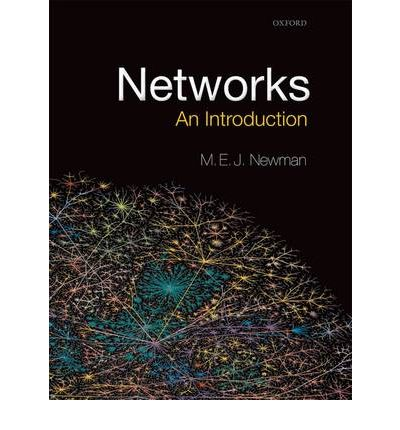
\includegraphics[width = 0.6\columnwidth]{networks_book.jpeg}
    \note{Most material is covered in this book}
\end{frame}
%-------------------------
%--------------------------------------
\begin{frame}
    \frametitle{Networks/Graphs}
    \begin{columns}
        \column{0.45\linewidth}
            \centering
            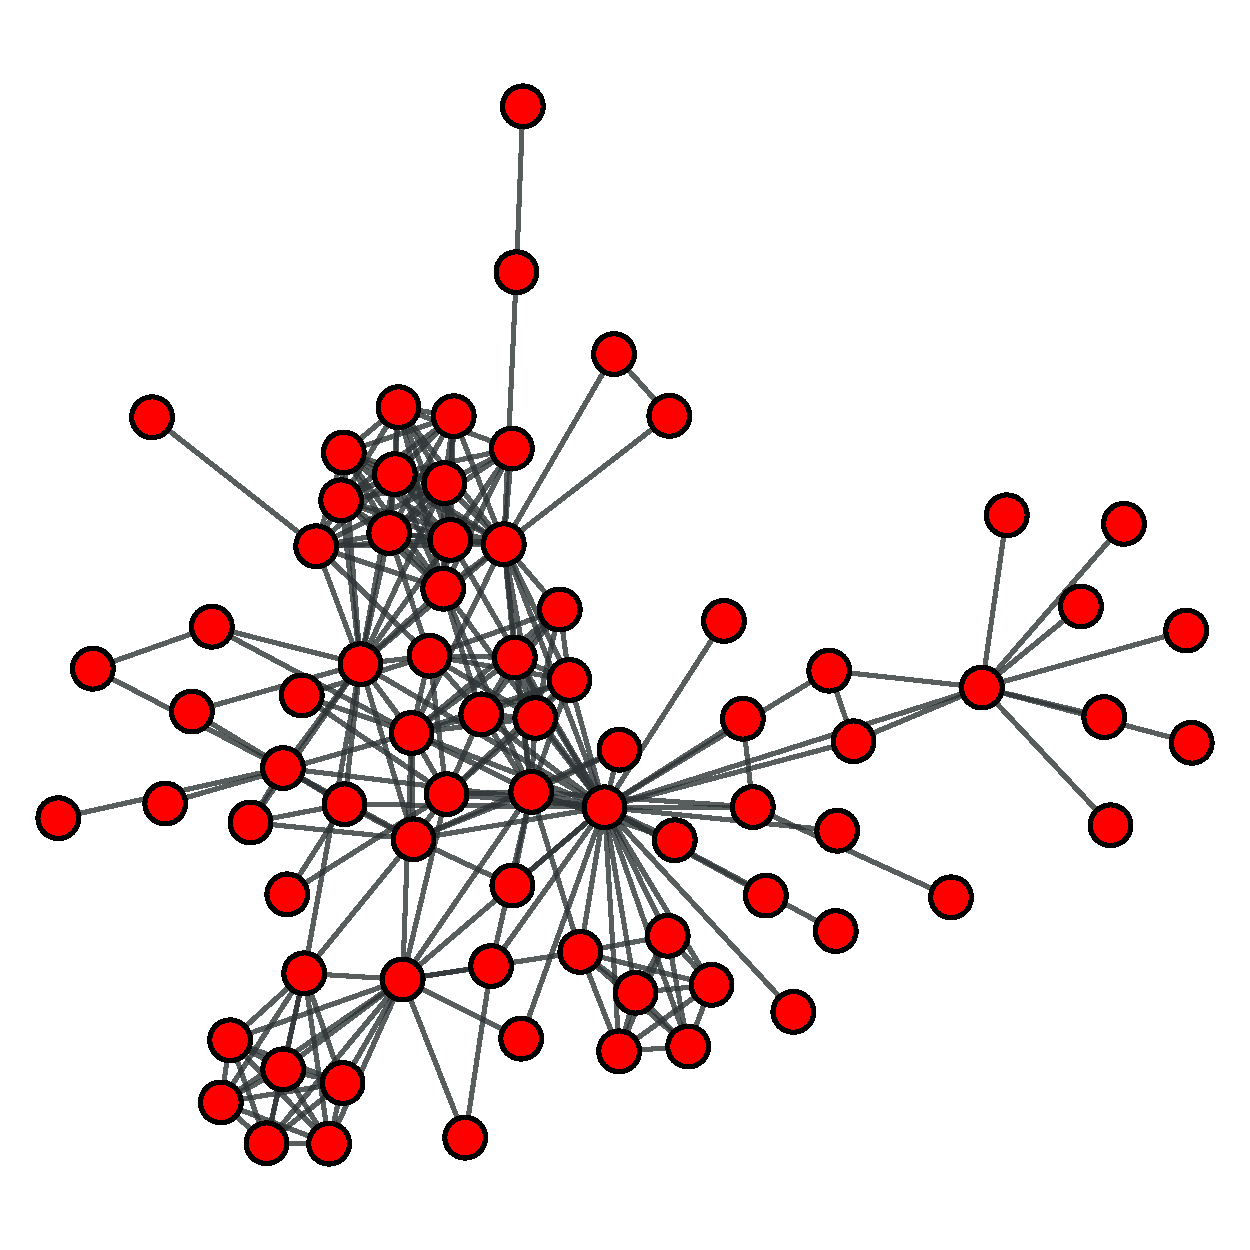
\includegraphics[width=\columnwidth]{lesmis.pdf}
        \column{0.58\linewidth}
            \begin{itemize}
                \setlength\itemsep{2em}
                \item{Points connected by lines}
                \item{Points: nodes/vertices/actors}
                \item{Lines: links/edges/ties}
            \end{itemize}
    \end{columns}
\end{frame}
%--------------------------------------
%--------------------------------------
\begin{frame}
    \frametitle{Real-world networks}
    \begin{itemize}
        \setlength\itemsep{1em}
            \item{{\bf Social}: Facebook, Friendships, Scientific collaborations}
            \item{{\bf Biological}: Human brain, Metabolic reactions }
            \item{{\bf Technological}: Internet, World-Wide-Web}
            \item{{\bf Transport}: Airports-Air routes, Cities-Highways}
    \end{itemize}
\end{frame}
%--------------------------------------
%--------------------------------------
%\begin{frame}
%    \frametitle{Real-world networks}
%    \begin{figure}
%        \begin{center}
%            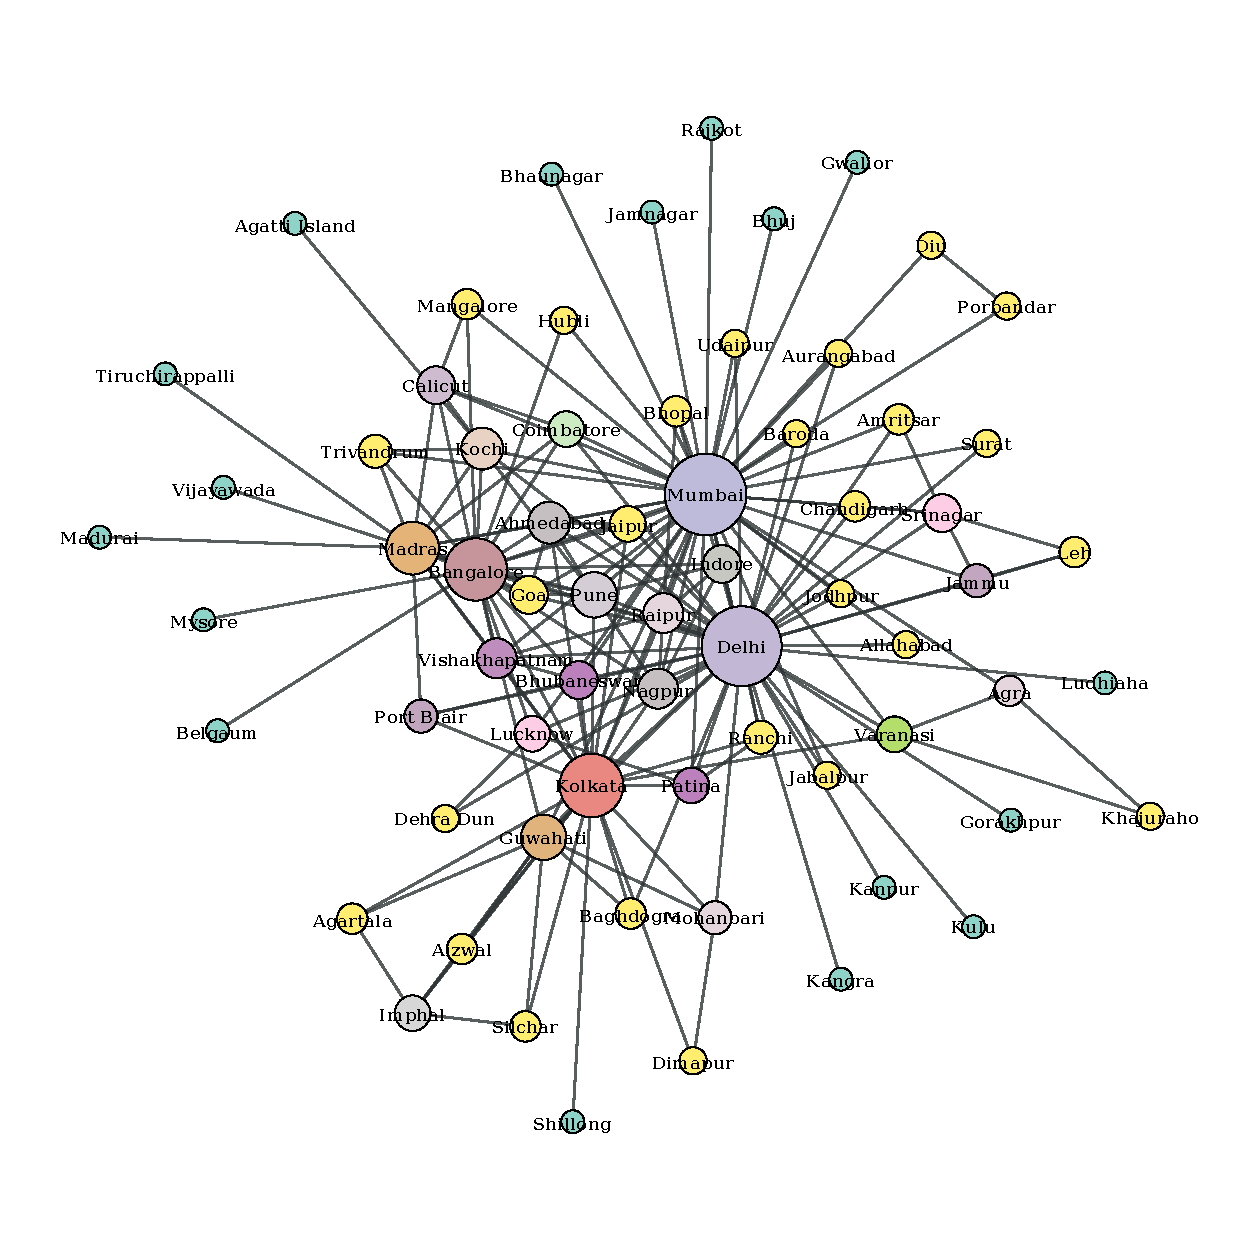
\includegraphics[width=0.8\columnwidth]{airports_network_India.pdf}
%        \end{center}
%    \end{figure}
%\end{frame}
%--------------------------------------
%--------------------------------------
\begin{frame}
    \frametitle{Two-questions}
        \begin{center}
            {\huge What are the nodes?}\\
            \vspace{5em}
            {\huge What are the links?}
        \end{center}
\end{frame}
%--------------------------------------
%--------------------------------------
\begin{frame}
    \frametitle{Is this a network?}

\begin{figure}
    \begin{center}
        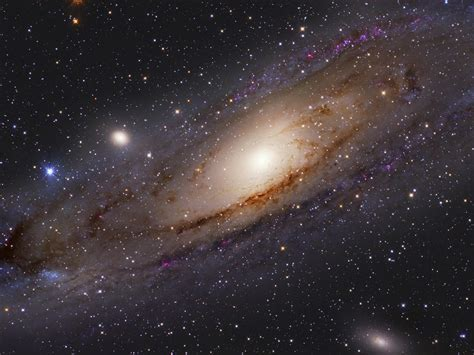
\includegraphics[width=0.6\columnwidth]{galaxy.jpeg}
    \end{center}
\end{figure}

\end{frame}
%--------------------------------------
%--------------------------------------
\begin{frame}
    \frametitle{Is this a network?}
\begin{figure}
    \begin{center}
        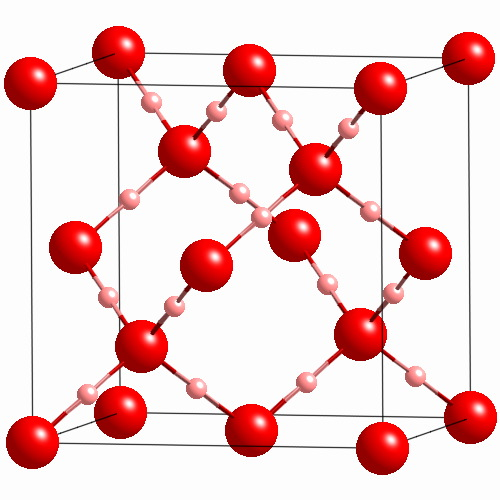
\includegraphics[width=0.4\columnwidth]{crystal.jpeg}
    \end{center}
\end{figure}
\end{frame}
%--------------------------------------
%--------------------------------------
\begin{frame}
    \frametitle{Is this a network?}
\begin{figure}
    \begin{center}
        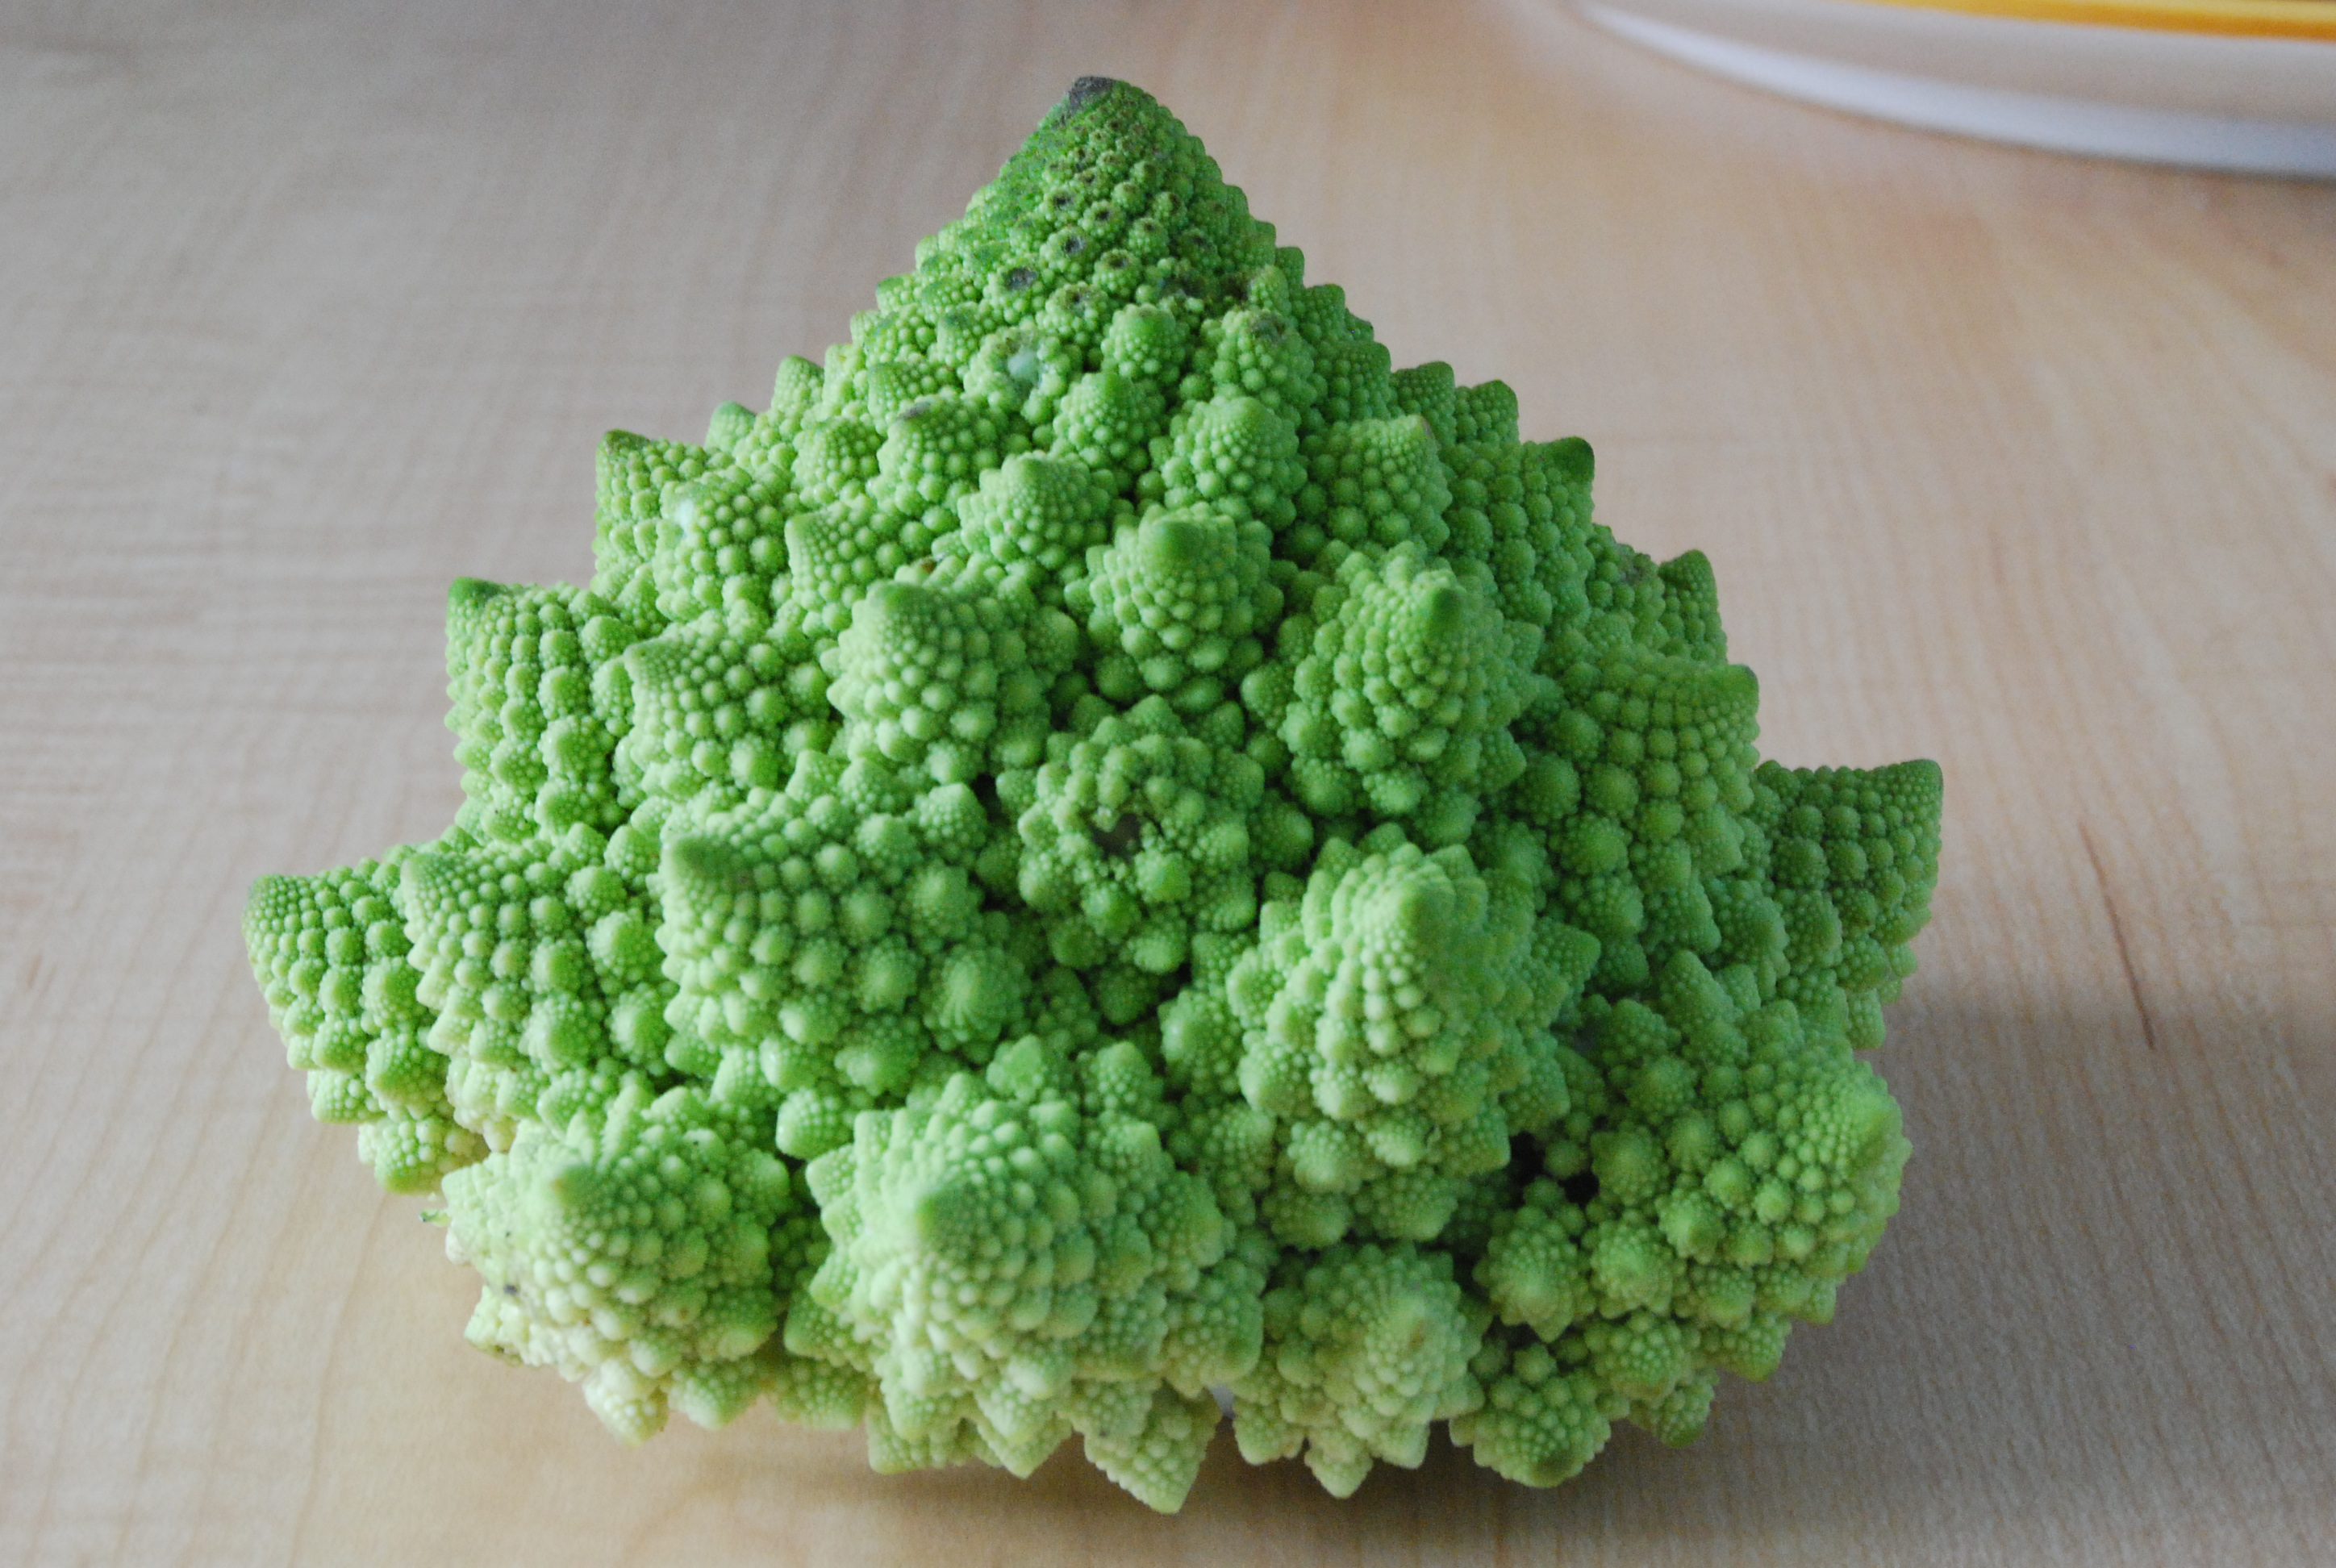
\includegraphics[width=0.7\columnwidth]{cauliflower.jpeg}
    \end{center}
\end{figure}
\end{frame}
%--------------------------------------
%--------------------------------------
\begin{frame}
    \frametitle{When is a network description useful?}
    \begin{itemize}
    \setlength\itemsep{1em}
        \item{Sparse data}
        \item{Lack of regularity}
        \item{Lack of a better model}
    \end{itemize}
\end{frame}
%--------------------------------------
%-------------------------
\begin{frame}
    \frametitle{Adjacency matrix}
\vspace{20pt}
\footnotesize
Adjacency matrix: Binary matrix of size $N \times N$
\begin{equation*}
A_{ij} = \begin{cases}
1 & \text{$i$ and $j$ connected}\\
0 & \text{$i$ and $j$ not connected}
\end{cases}
\end{equation*}
\vspace{10pt}

\note{For undirected networks, A is symmetric}
\begin{figure}
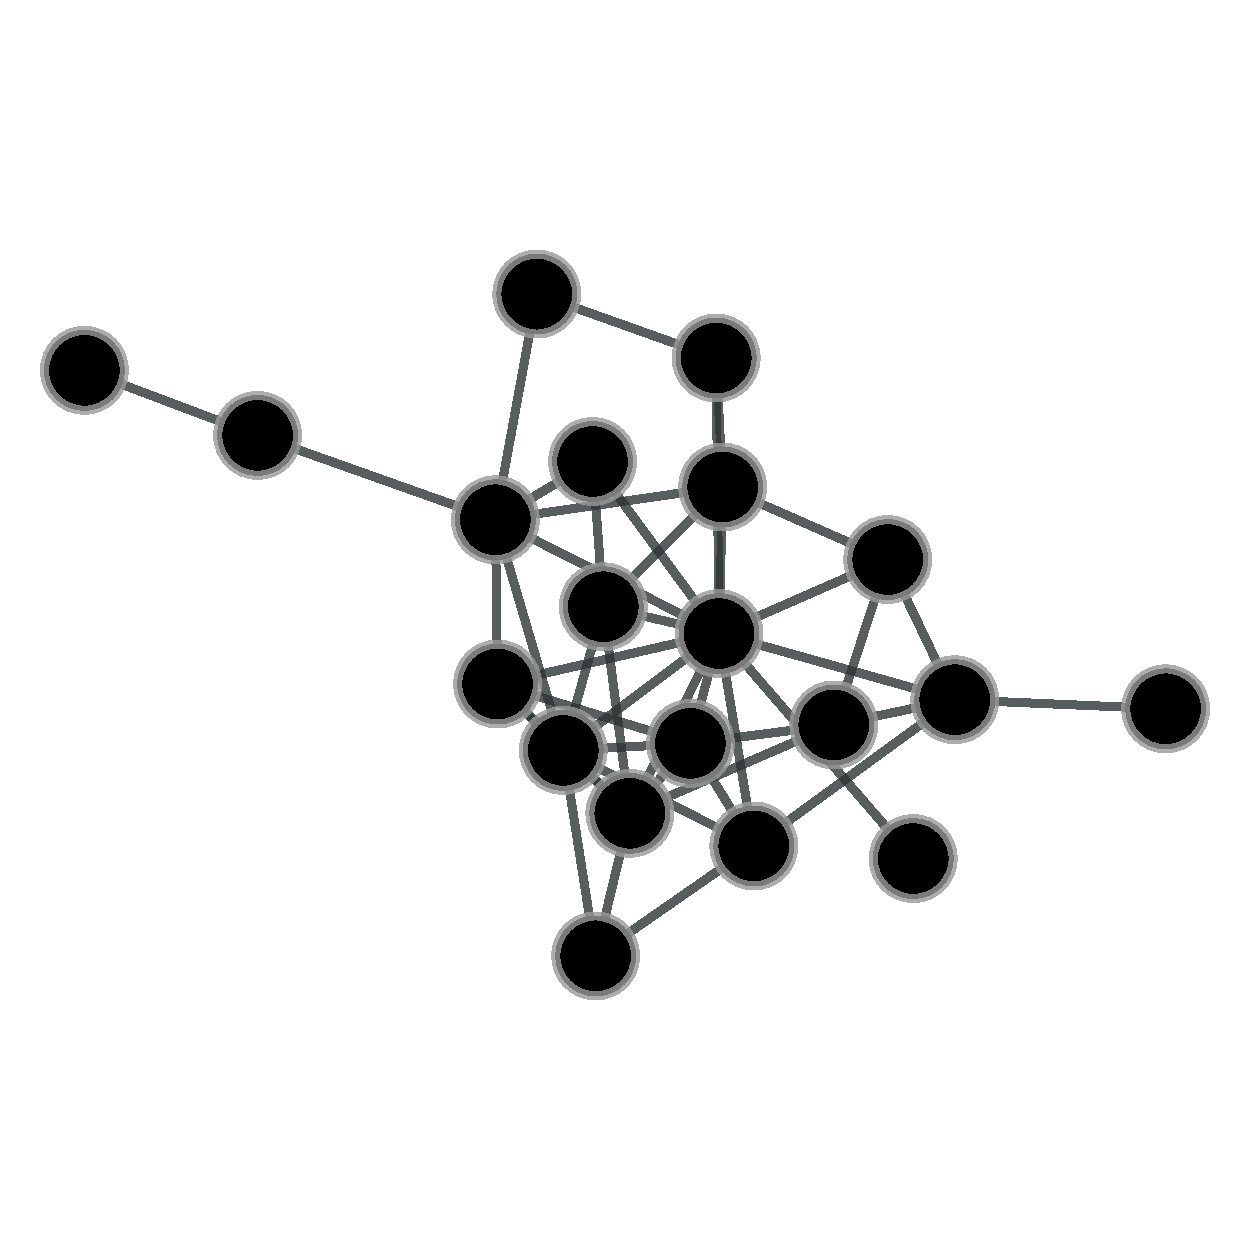
\includegraphics[width=0.5\columnwidth, trim = 0 0 0 100]{network.pdf}
\end{figure}
\end{frame}
%-------------------------
%-------------------------
\begin{frame}
    \frametitle{Average degree}
    Degree of a vertex: 
    \begin{equation*}
    k_i = \sum\limits_{j}A_{ij} 
    \end{equation*}

    Average degree of the network: 
    $$<k> = \sum\limits_{i}k_i$$
\end{frame}
%-------------------------
%--------------------------------------
\begin{frame}
    \frametitle{Complex networks}
    \begin{itemize}
    \setlength\itemsep{2em}
       \item{\Large {\bf Complex}: Edge of order and randomness}
        \pause
        \item{\Large {\bf Structure vs Processes}
            \begin{itemize}
            \setlength\itemsep{1em}
                \item{Spreading of epidemics, rumors, ideas}
                \item{Traffic}
                \item{Neuronal dynamics}
            \end{itemize}
        }
        \pause
        \item{\Large \bf Structure is intersting on its own!}
    \end{itemize}
\end{frame}
%--------------------------------------
%--------------------------------------
\begin{frame}
    \frametitle{Simplifications}
    \begin{columns}
        \column{0.7\linewidth}
            \centering
            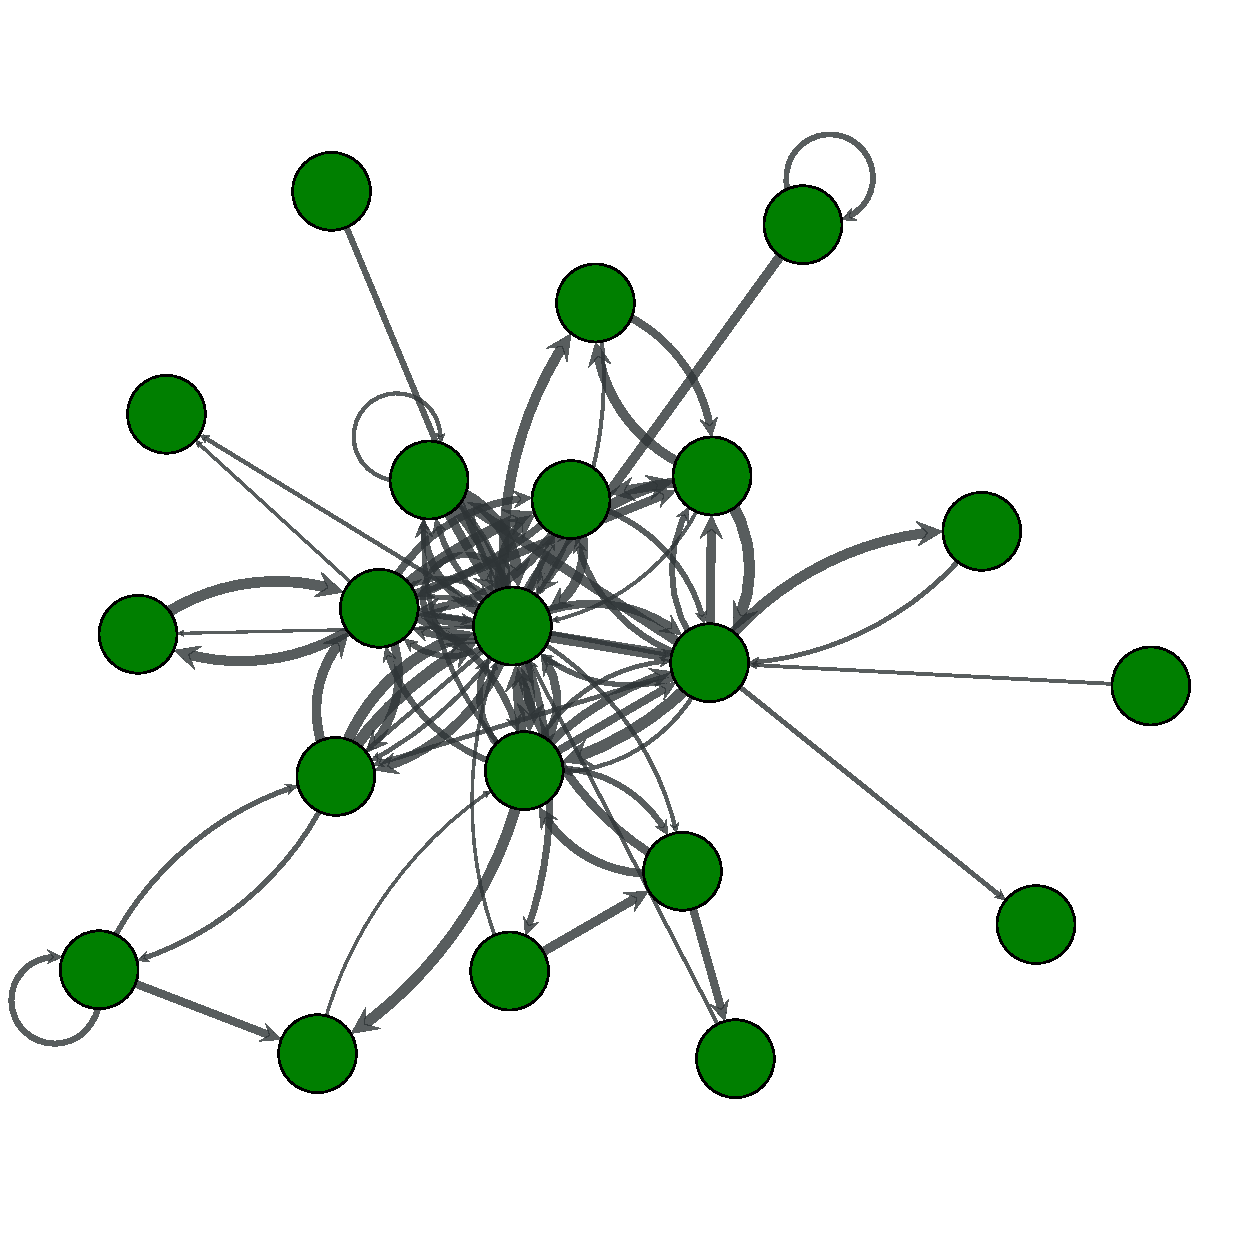
\includegraphics[width=0.9\columnwidth]{weighted_directed_nonsimple2.pdf}
        \column{0.4\linewidth}
            \centering
            \begin{itemize}
            \setlength\itemsep{1em}
                \item{Simple}
                \item{Undirected}
                \item{Unweighted}
                \item{Static}
            \end{itemize}
    \end{columns}
\end{frame}
%--------------------------------------

%----------------------------------------
\begin{frame}
    \frametitle{Simplifications}
    \centering
    {\Large \bf The largest component}
    \begin{figure}
        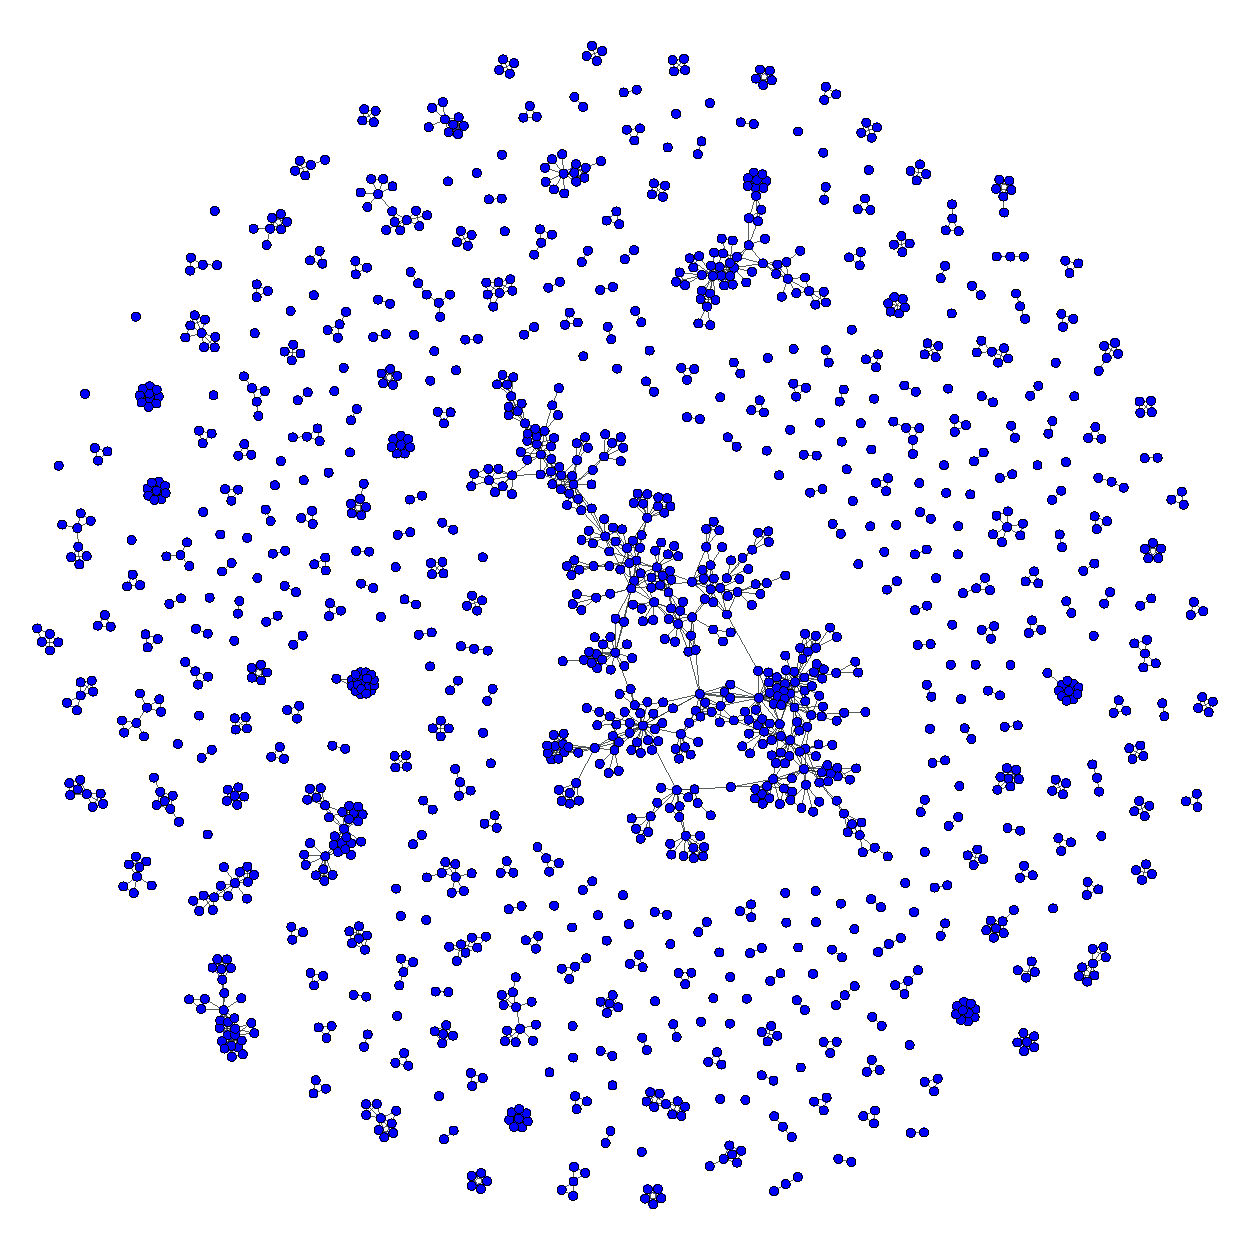
\includegraphics[width=0.7\columnwidth]{netscience.pdf}
    \end{figure}
\end{frame}
%----------------------------------------

%--------------------------------------
\begin{frame}
    \frametitle{Large-scale structure of complex networks}
    \begin{itemize}
    \setlength\itemsep{1em}
        \item{{\bf Small-scale structures}: 
            \begin{itemize}
                \item{degree}
                \item{local clustering}
                \item{centrality scores}
            \end{itemize}
}
        \item{{\bf Meso-scale structures}: 
            \begin{itemize}
                \item{motifs}
                \item{vertex similarity}
                \item{rich-club effect}
            \end{itemize}
}
        \item{{\bf Large-scale structures}: 
                \begin{itemize}
                    \item{\bf components and percolation}
                    \item{small-world effect}
                    \item{ranking}
                    \item{{\bf degree distribution}}
                    \item{{\bf assortative mixing}}
                    \item{{\bf community structure}}
                \end{itemize}
}
    \end{itemize}
    
\end{frame}
%--------------------------------------
%--------------------------------------
\begin{frame}
    \frametitle{Degree-distrbution}
    \begin{columns}
        \column{0.5\linewidth}
        \centering
        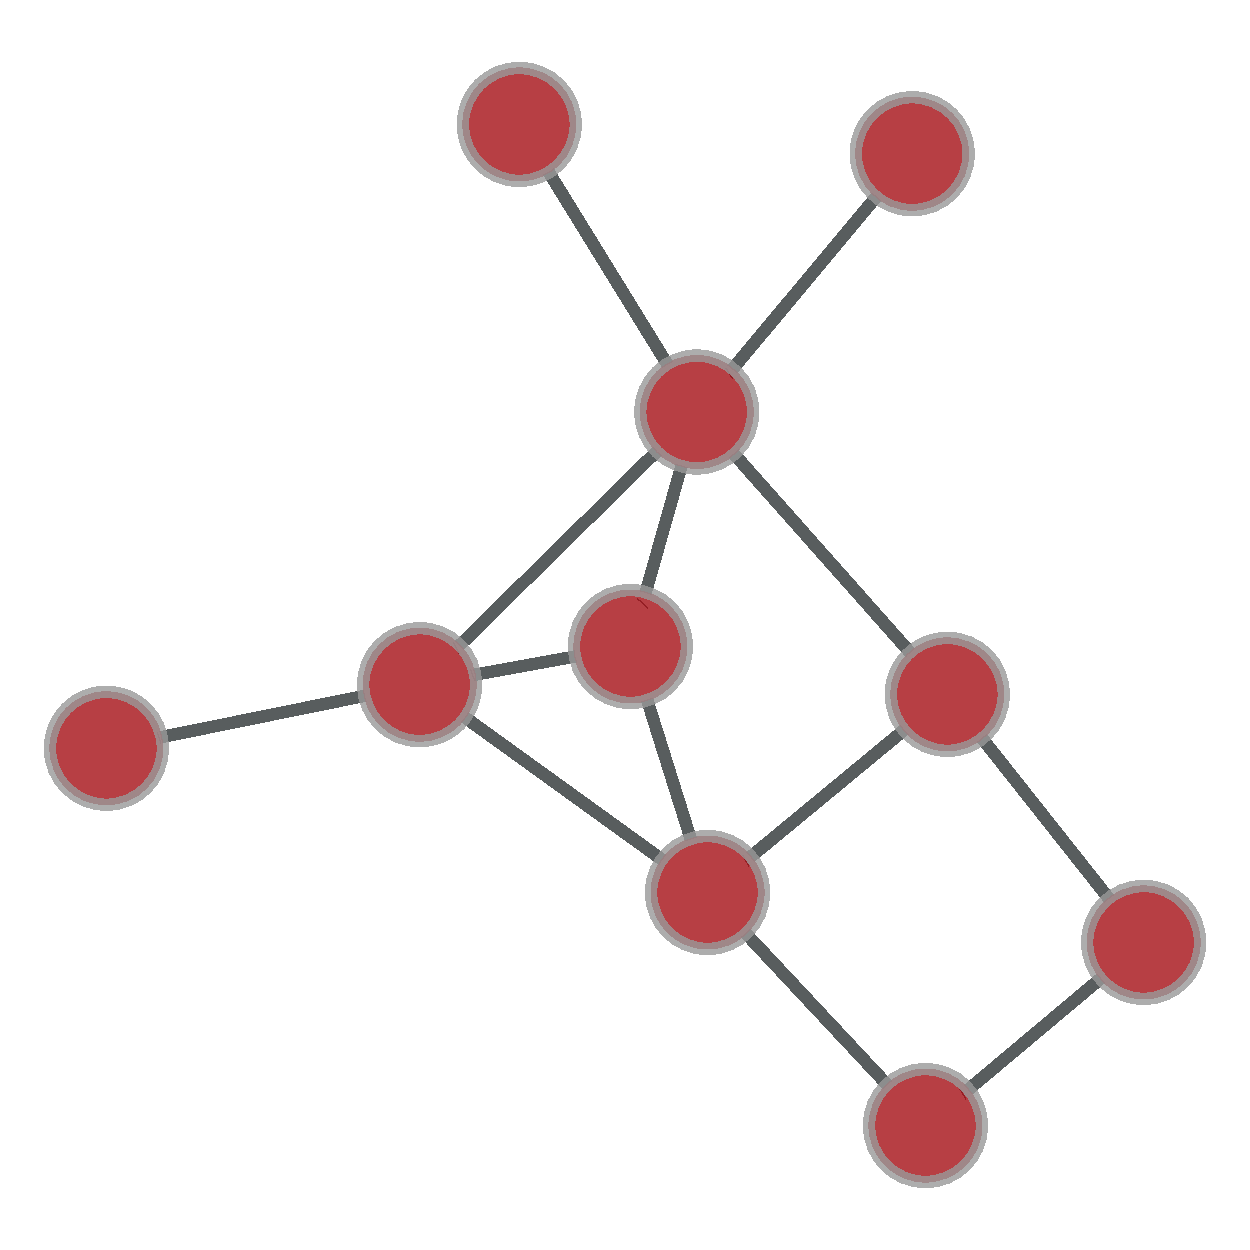
\includegraphics[width=\columnwidth]{small_graph.pdf}
        \column{0.5\linewidth}
        \centering
        Total $10$ vertices

        $$p_{1} = \frac{3}{10}$$
        $$p_{2} = \frac{2}{10}$$
        $$p_{3} = \frac{2}{10}$$
        $$p_{4} = \frac{2}{10}$$
        $$p_{5} = \frac{1}{10}$$
    \end{columns}
\end{frame}
%--------------------------------------
%--------------------------------------
\begin{frame}
    \frametitle{Degree distribution}
    \begin{columns}
        \column{0.6\linewidth}
        \centering
        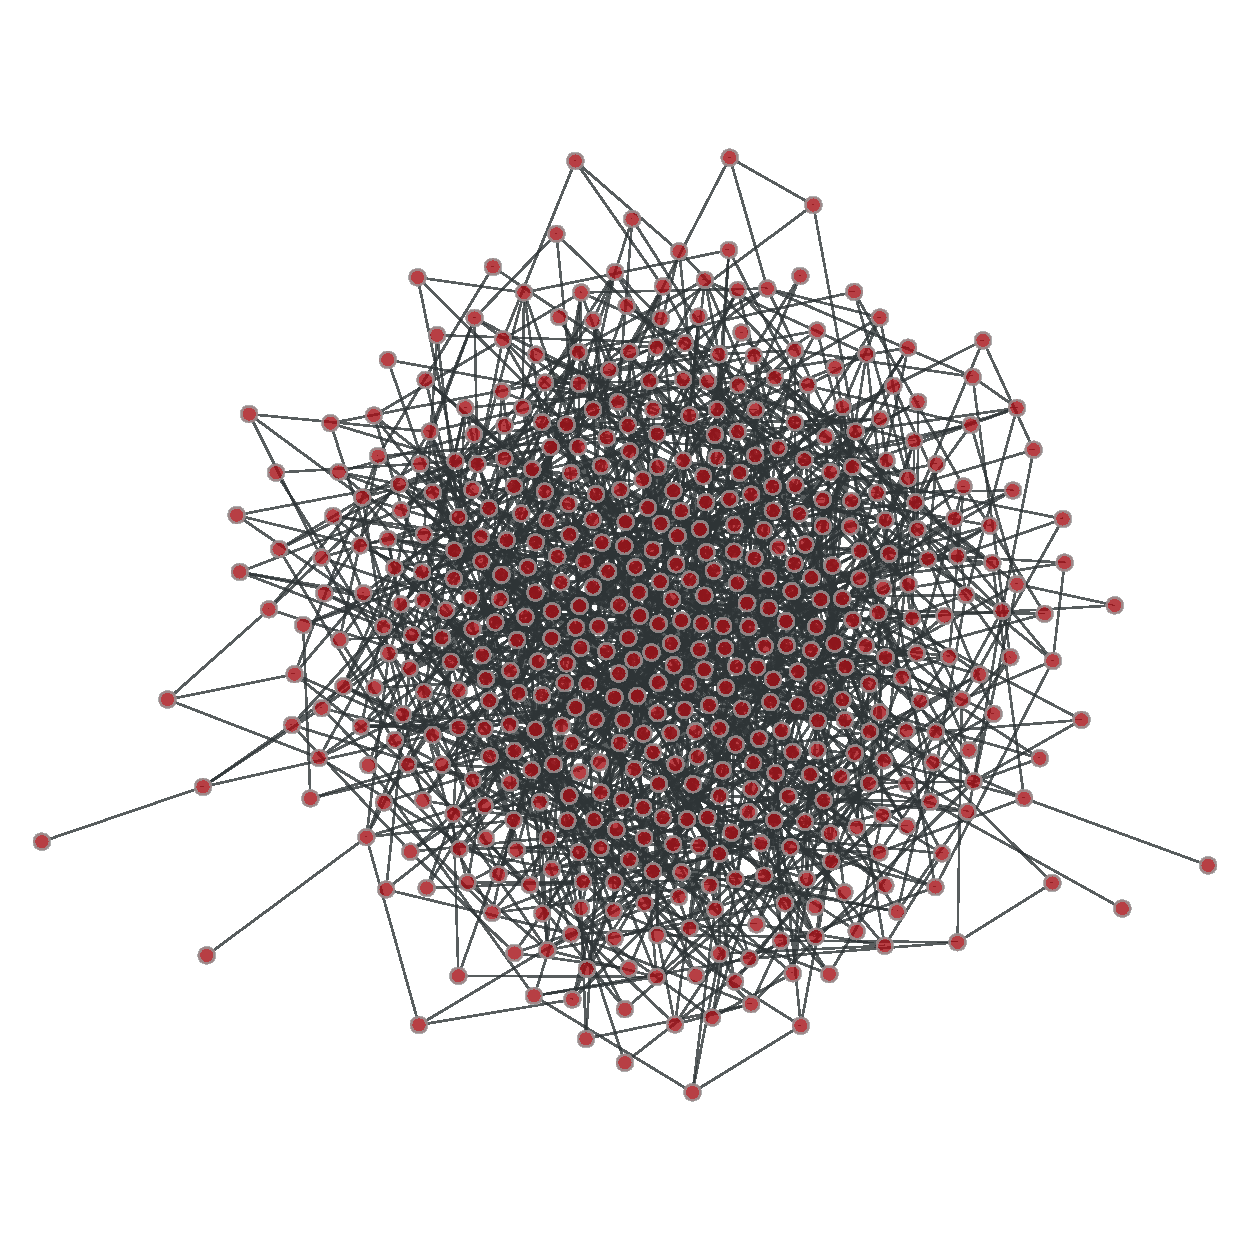
\includegraphics[width=\columnwidth]{big_graph.pdf}

        \column{0.6\linewidth}
        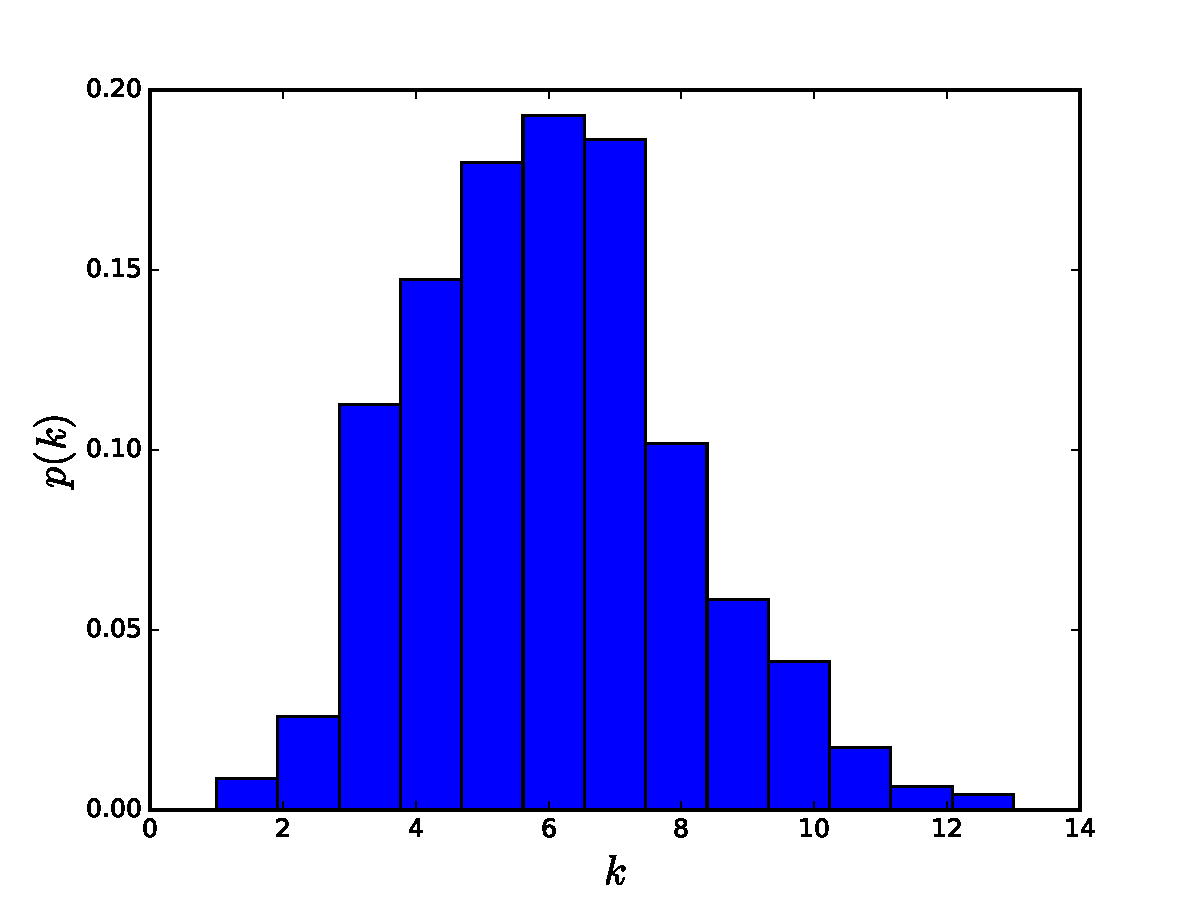
\includegraphics[width=\columnwidth]{deg_distri_example.pdf}
        \centering
    \end{columns}
\end{frame}
%--------------------------------------
%--------------------------------------
\begin{frame}
    \frametitle{Metabolic network of the worm C-elegans}
    \begin{columns}
        \column{0.6\linewidth}
        \centering
        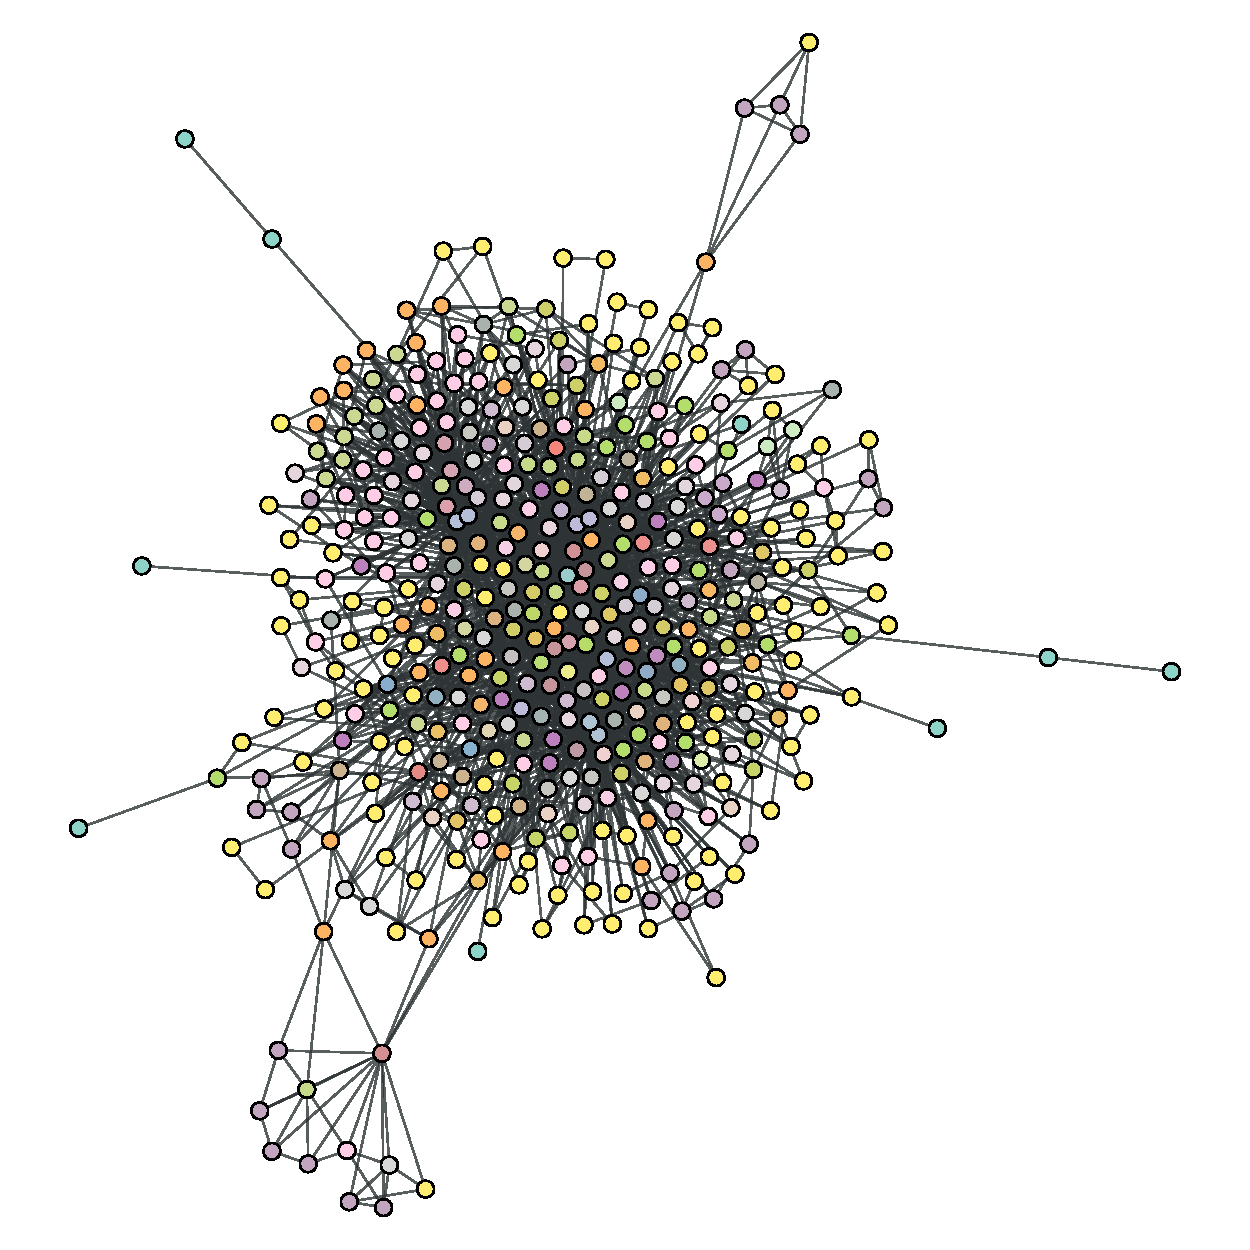
\includegraphics[width=\columnwidth]{celegans_metabolic.pdf}
        \column{0.6\linewidth}
        \centering
        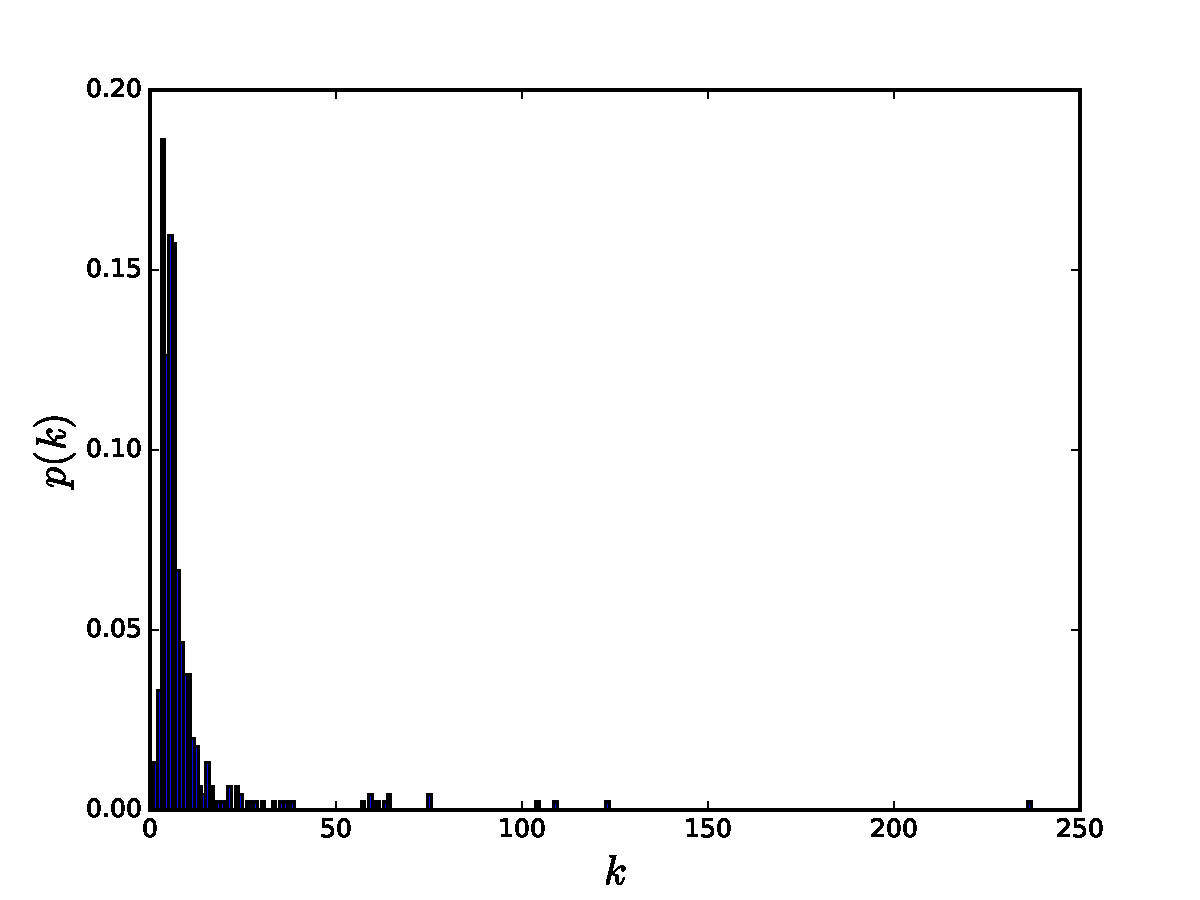
\includegraphics[width=\columnwidth]{deg_distri_celegans_metabolic.pdf}
    \end{columns}
\end{frame}
%--------------------------------------
%--------------------------------------
\begin{frame}
    \frametitle{Degree distribution of the real world networks}
    \begin{columns}
        \column{0.6\linewidth}
        \centering
        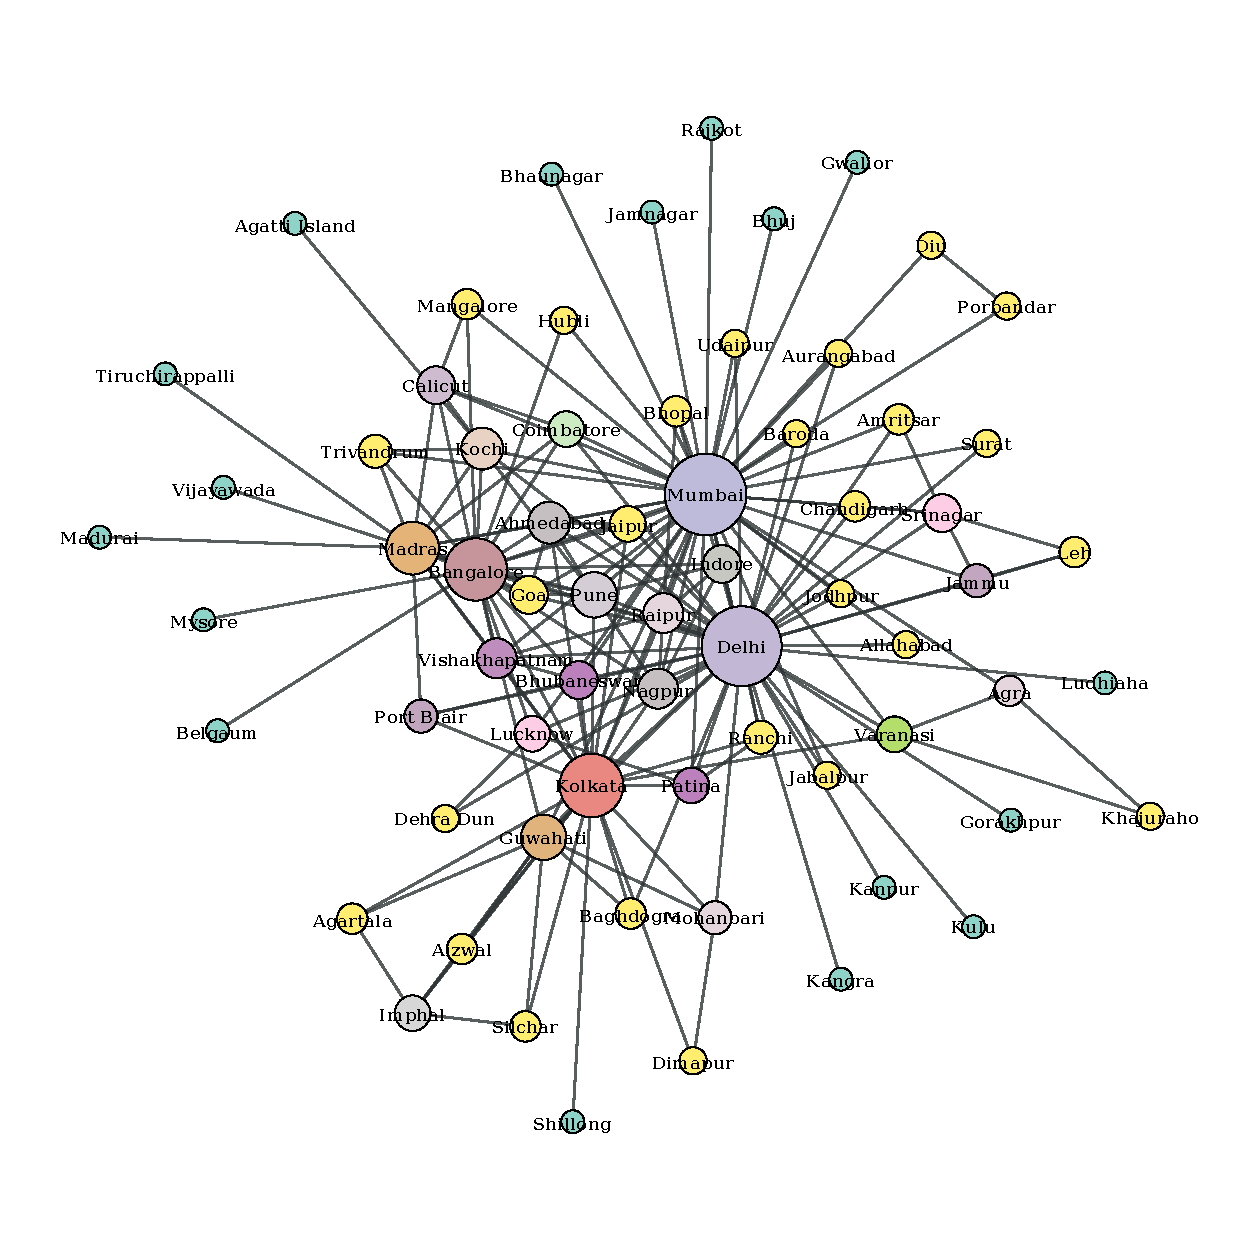
\includegraphics[width=\columnwidth]{airports_network_India.pdf}

        \column{0.6\linewidth}
        \centering
        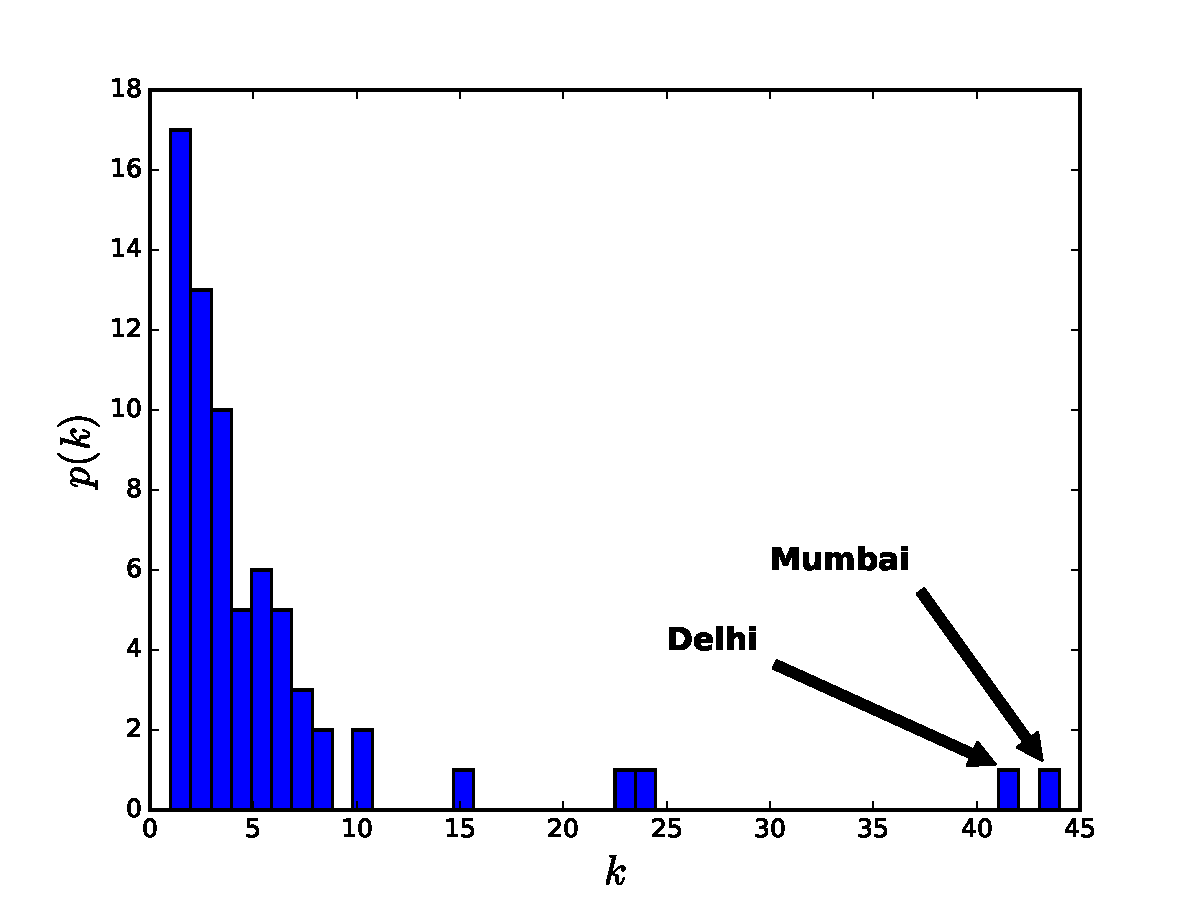
\includegraphics[width=\columnwidth,trim=30 0 0 0,clip=true]{deg_distri_india.pdf}
    
    \end{columns}
\end{frame}
%--------------------------------------
%--------------------------------------
\begin{frame}
    \frametitle{Degree distribution of the real-world networks}
    \begin{columns}
        \column{0.6\linewidth}
        \centering
        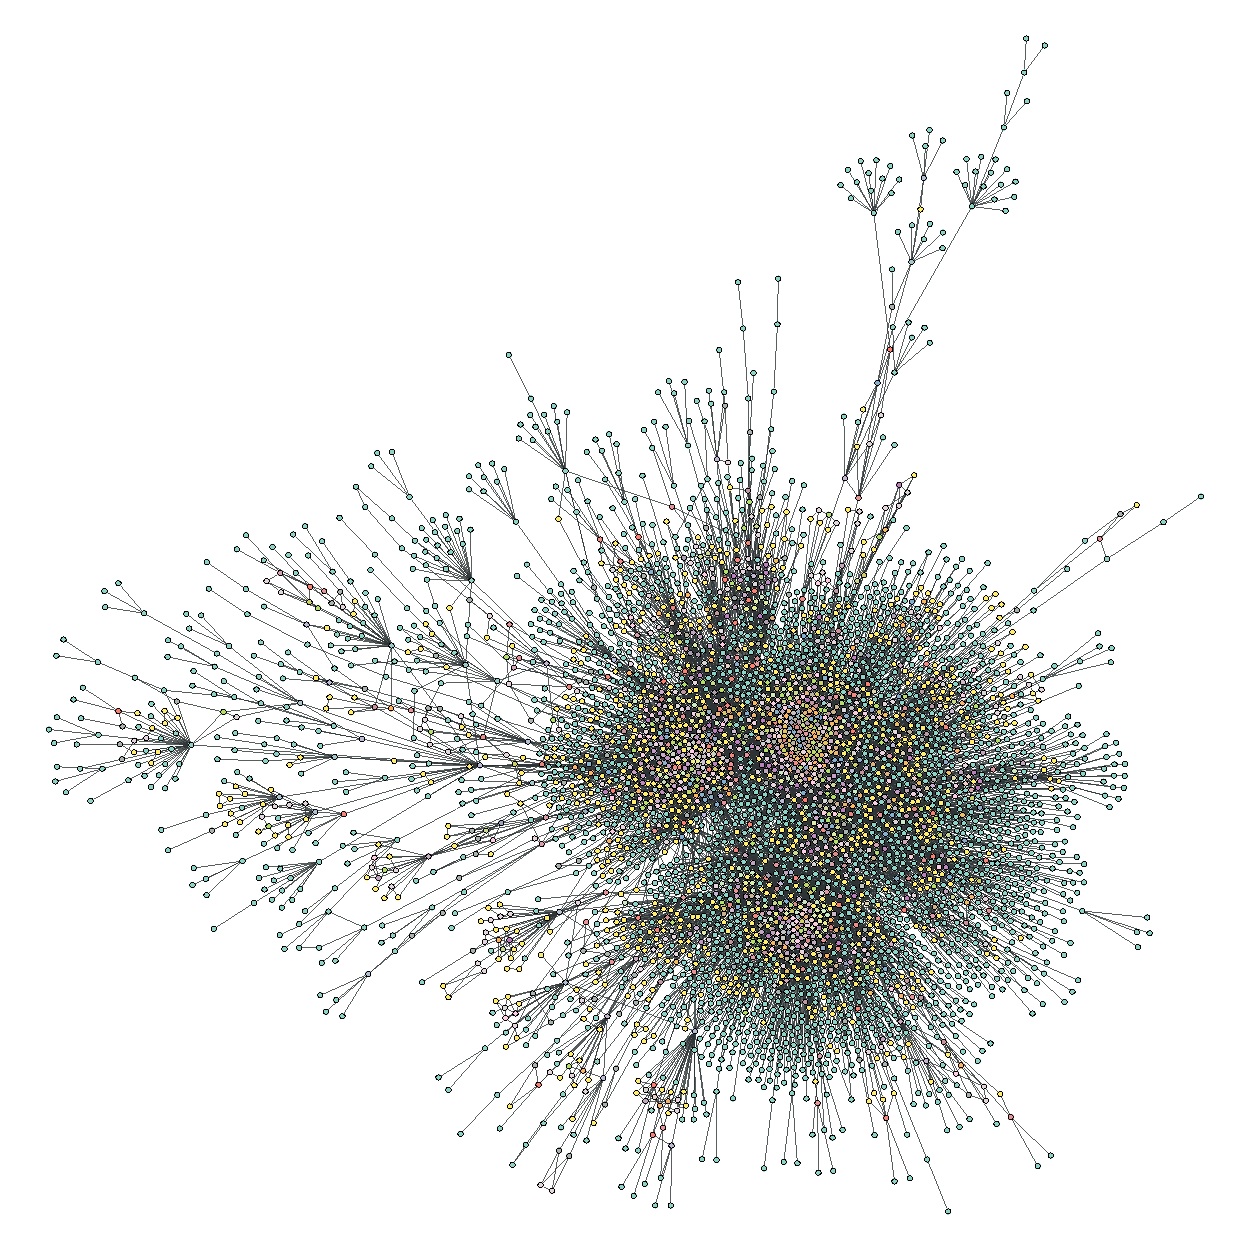
\includegraphics[width=\columnwidth]{airports_network_global.pdf}
        \column{0.6\linewidth}
        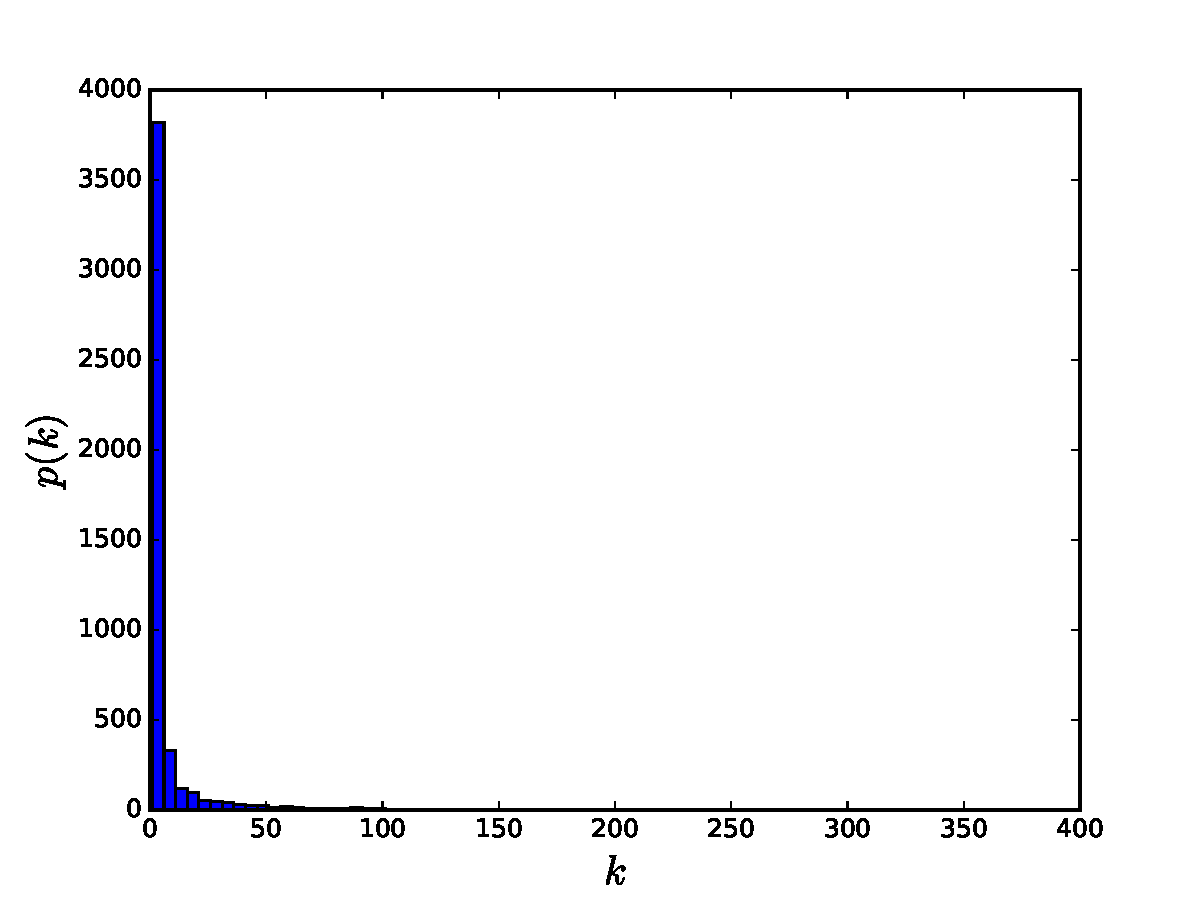
\includegraphics[width=\columnwidth]{deg_distri_global_airport.pdf}
        \centering
    \end{columns}
\end{frame}
%--------------------------------------
%--------------------------------------
\begin{frame}
    \frametitle{Power-laws and scale-free networks}
    \begin{columns}
        \column{0.7\linewidth}
        \centering
        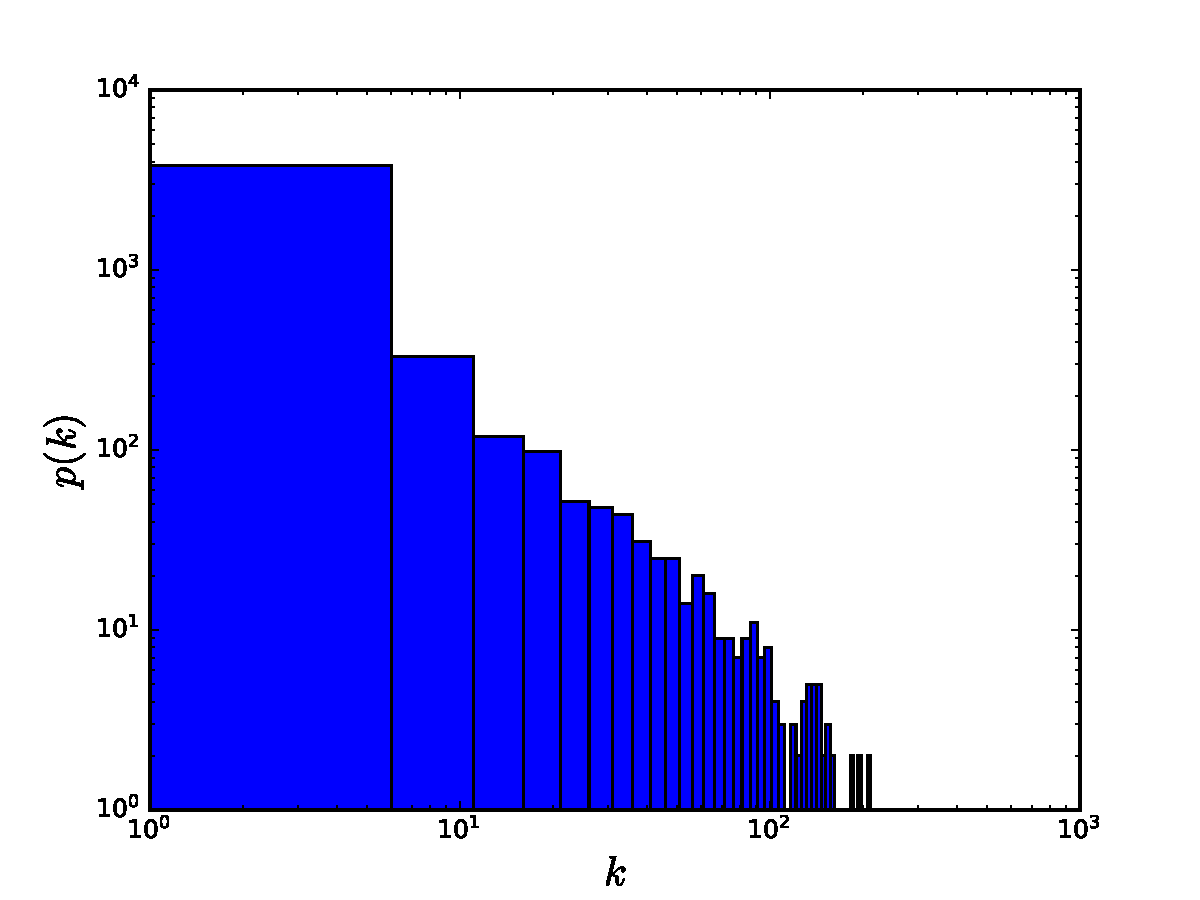
\includegraphics[width=\columnwidth]{deg_distri_global_airport_log.pdf}
        \column{0.4\linewidth}
        \centering
        $$\ln p(k) = -\alpha \ln k + c$$ 
        $$p(k) = Ck^{-\alpha}\quad\forall \ k > k_{\text{min}}$$

    \end{columns}
\end{frame}
%--------------------------------------
%-------------------------
%\begin{frame}
%    \frametitle{Detecting and visualizing power-laws}
%    \centering
%    How do we know that a given distribution is a power-law?
%    \begin{itemize}
%    \setlength\itemsep{1em}
%        \item{Plotting the distribution on a log-log scale}
%    \end{itemize}
%    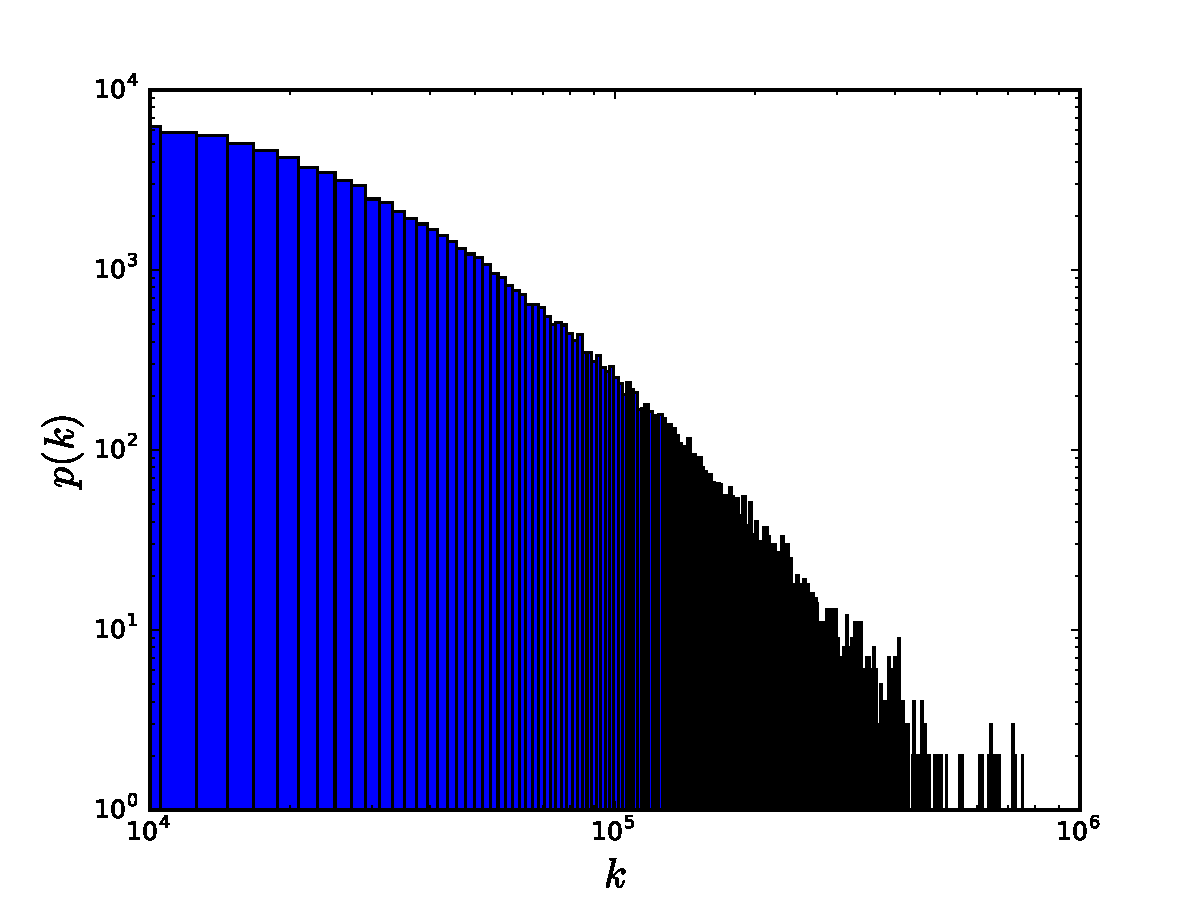
\includegraphics[width=0.8\columnwidth]{lognormal.pdf}
%    \note{lognormal}
%\end{frame}
%-------------------------
%-------------------------
\begin{frame}
    \frametitle{Detecting and visualizing power-laws}
    \centering
    How do we know that a given distribution is a power-law?
    \begin{itemize}
    \setlength\itemsep{1em}
        \item{Creating a log-log plot}
    \end{itemize}
    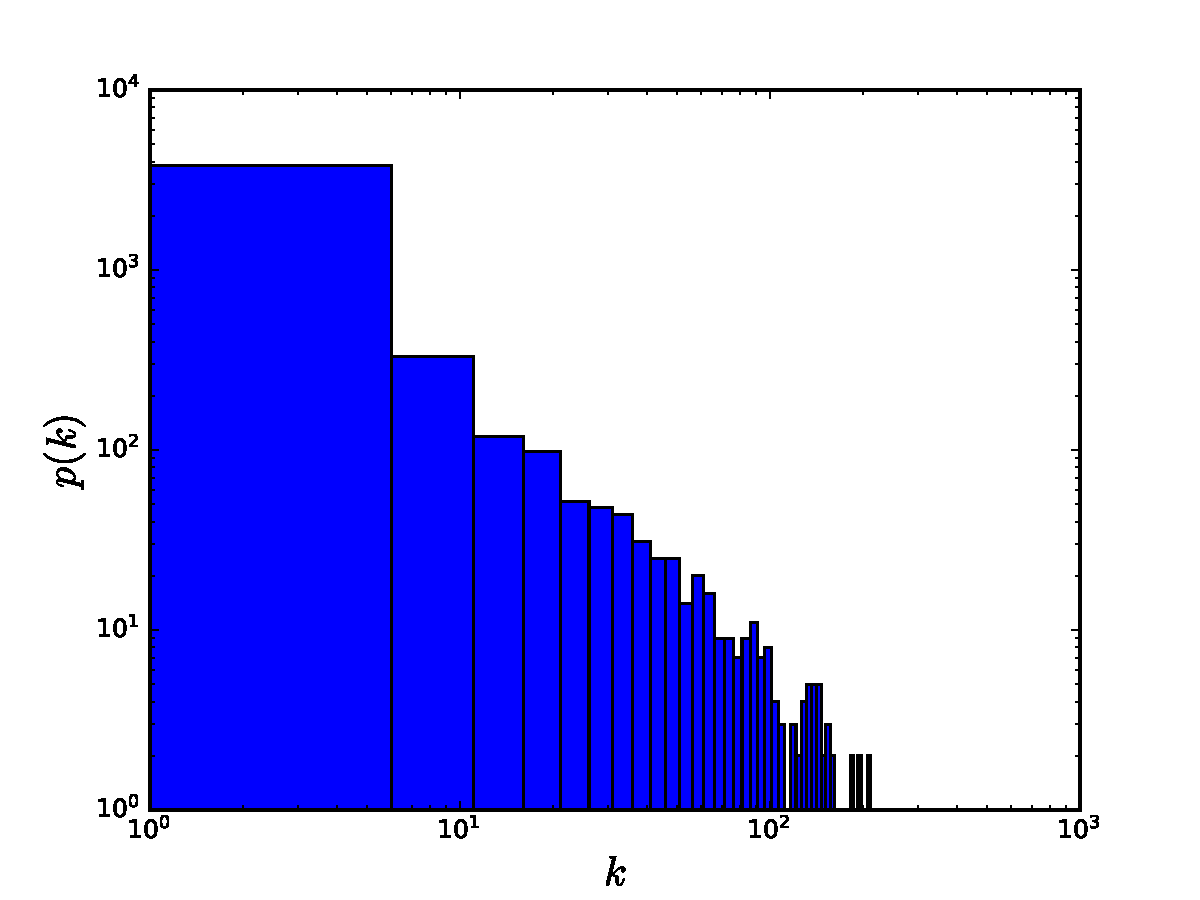
\includegraphics[width=0.8\columnwidth]{deg_distri_global_airport_log.pdf}
    \note{More imp question\\.\\log-log: objectively bad way}
\end{frame}
%-------------------------
%-------------------------
\begin{frame}
    \frametitle{Detecting and visualizing power-laws}
    \centering
    Power-law is tricky!
    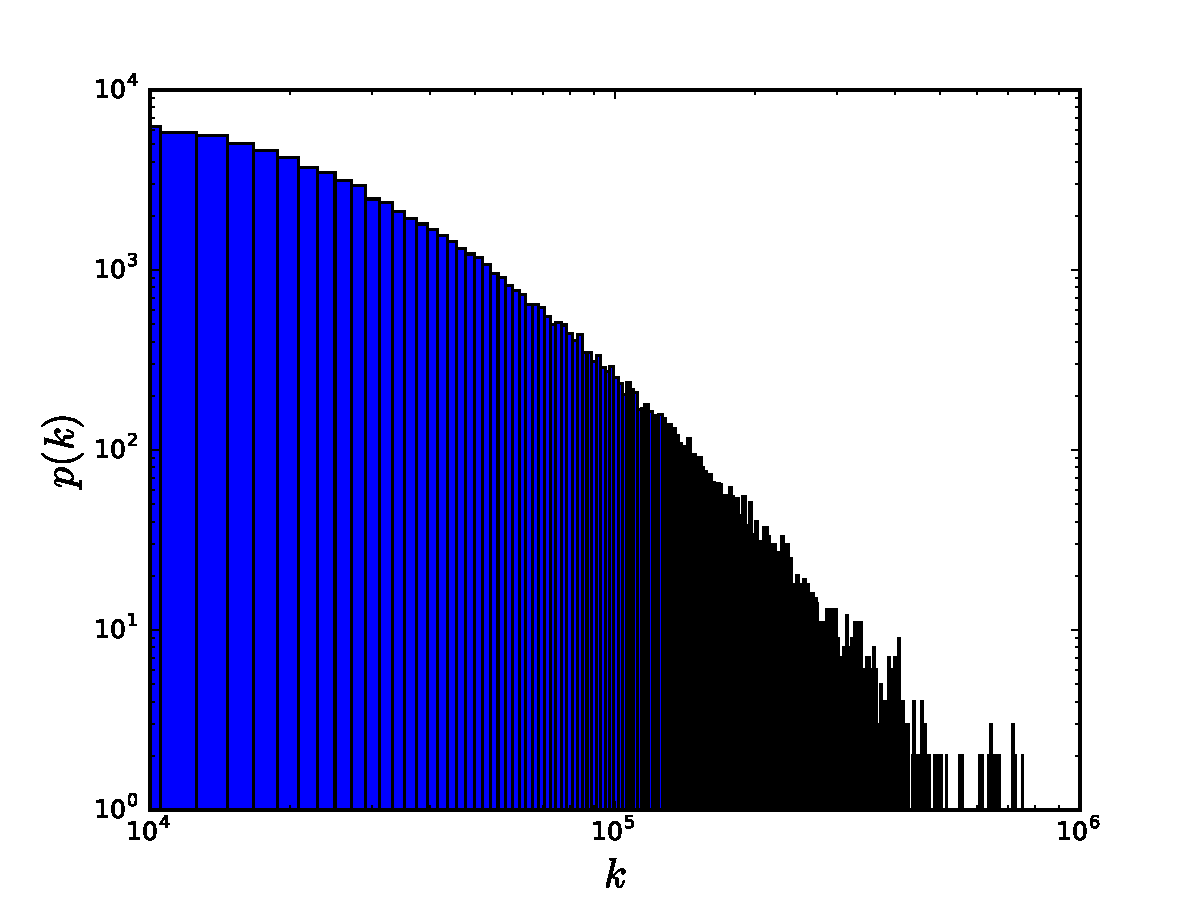
\includegraphics[width=0.8\columnwidth]{lognormal.pdf}
    \note{lognormal}
\end{frame}
%-------------------------
%-------------------------
\begin{frame}
    \frametitle{Detecting and visualizing power-laws}
    \centering
    \begin{itemize}
    \setlength\itemsep{1em}
        \item{Logarthmic binning: next bin is fixed multiple wider than the previous one}
        \item{Better but still noisy}
    \end{itemize}

\begin{figure}
    \begin{center}
        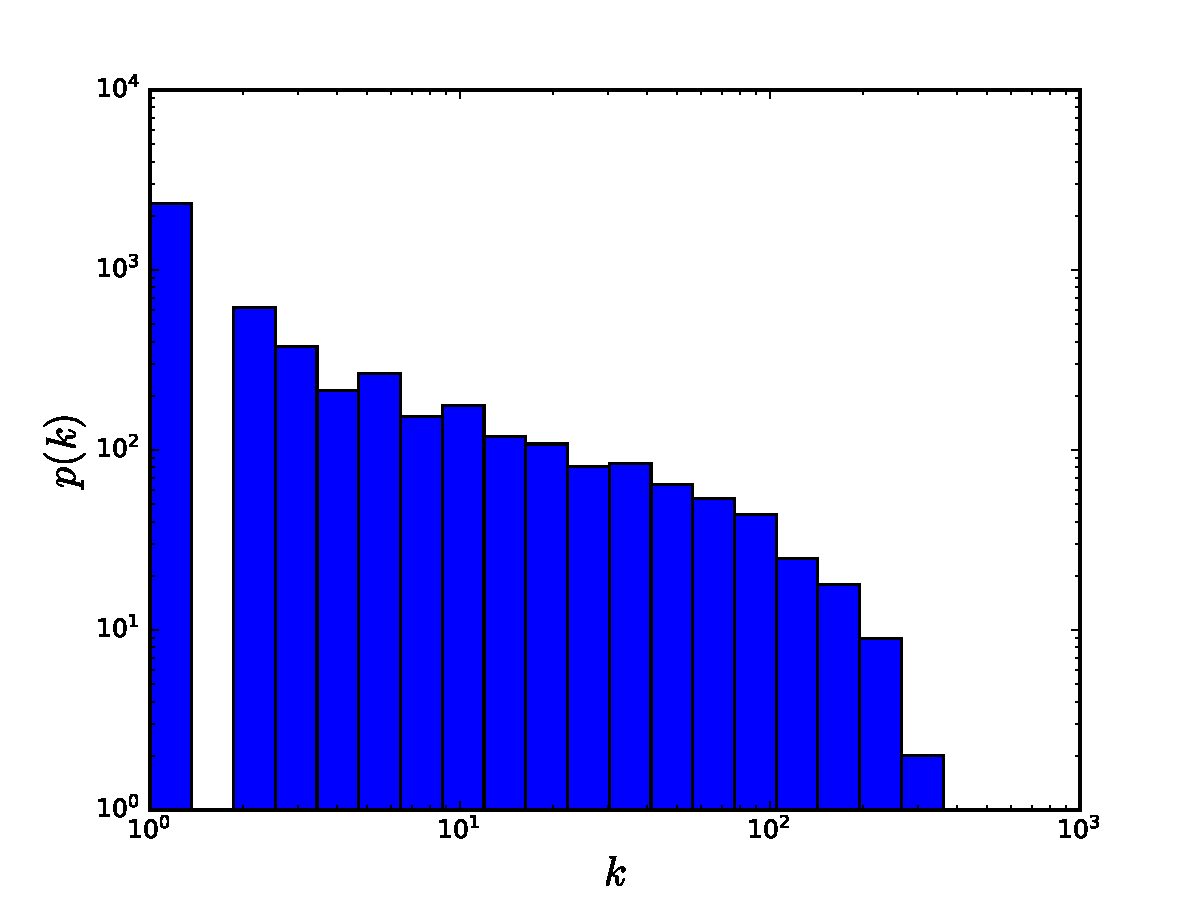
\includegraphics[width=0.8\columnwidth]{deg_distri_global_airport_log_logbins.pdf}
        \caption{\label{}}
    \end{center}
\end{figure}

\end{frame}
%-------------------------
%-------------------------
\begin{frame}
    \frametitle{Detecting and visualizing power-laws}
    \centering
    {\bf Cumulative distribution}
    $$P(k) = \sum\limits_{k^{\prime} = k}^\infty p(k^{\prime})$$

    $$P(k) = C\sum\limits_{k^{\prime} = k}^\infty {k^{\prime}}^{-\alpha} \approx C\int_k^\infty {k^{\prime}}^{-\alpha}dk^{\prime} = \frac{C}{\alpha-1}k^{-(\alpha-1)}$$
\note{$\alpha > 1$ and power-law slowly decreases\\}
    \note{Needs no binning!}
\end{frame}
%-------------------------
%--------------------------------------
%\begin{frame}
%    \frametitle{Detecting and visualizing power-laws}
%    \centering
%    {\bf The global network of airports}
%    
%    \vspace{2em}
%    \begin{columns}
%    \column{0.35\linewidth}
%        \centering
%        {\bf Log-log scale}
%        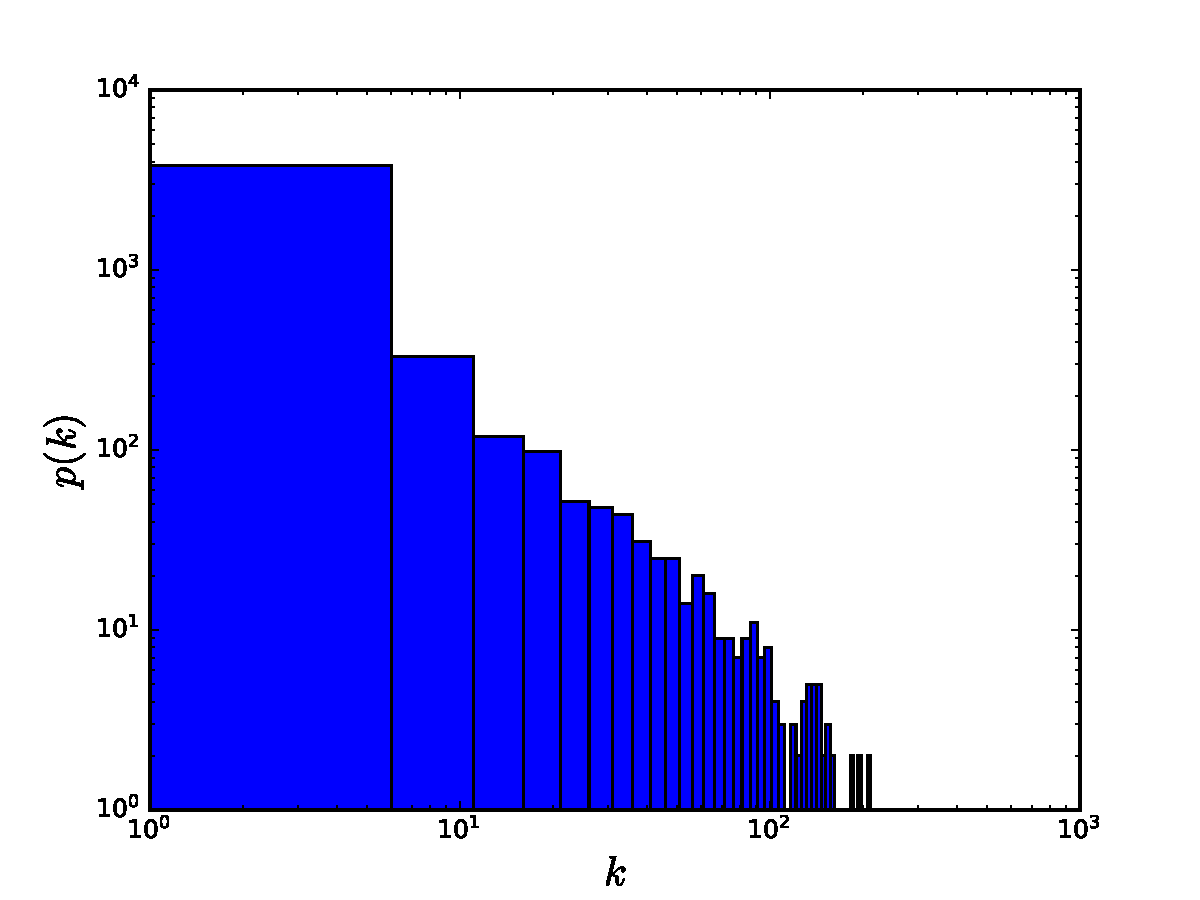
\includegraphics[width=\columnwidth]{deg_distri_global_airport_log.pdf}
%    \column{0.35\linewidth}
%        \centering
%        {\bf Logarthmic bins}
%        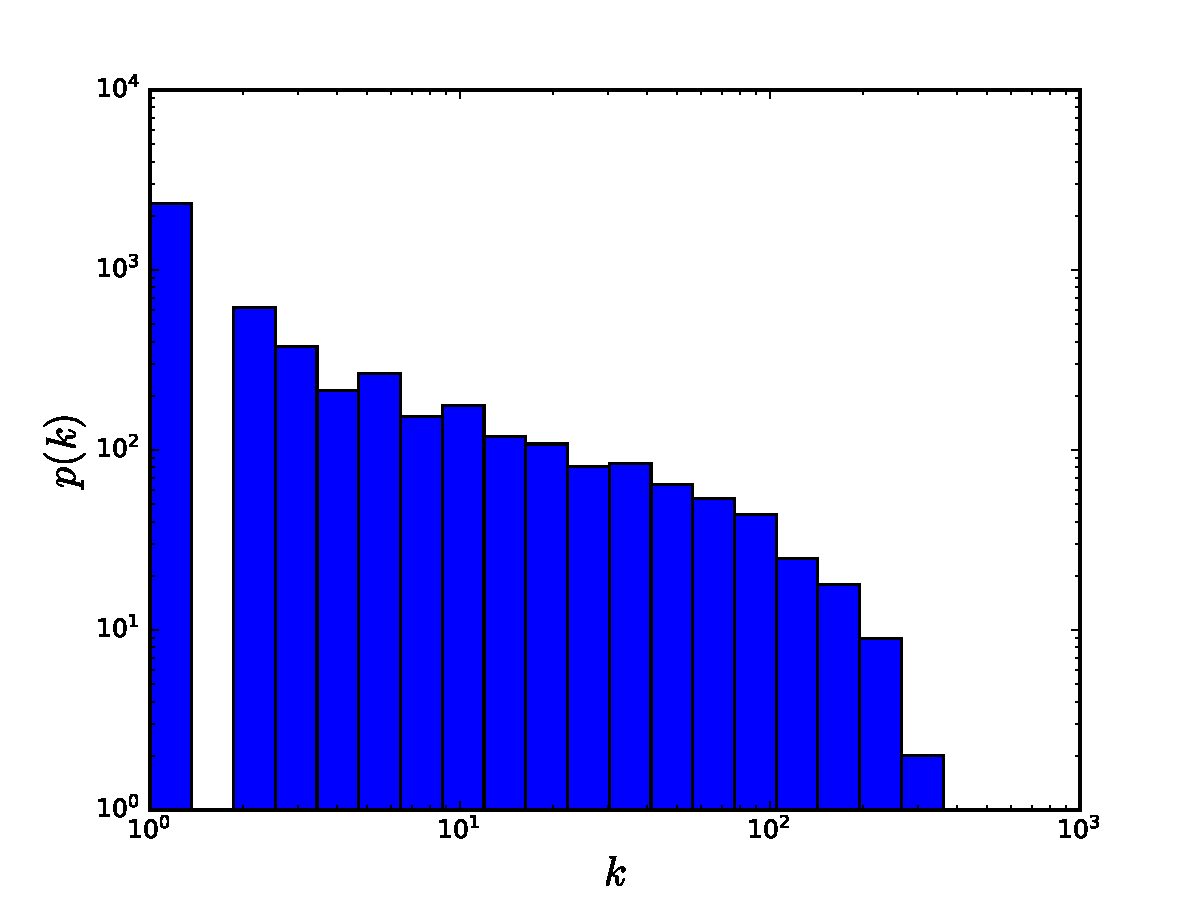
\includegraphics[width=\columnwidth]{deg_distri_global_airport_log_logbins.pdf}
%    \column{0.35\linewidth}
%        \centering
%        {\bf Cumulative }
%        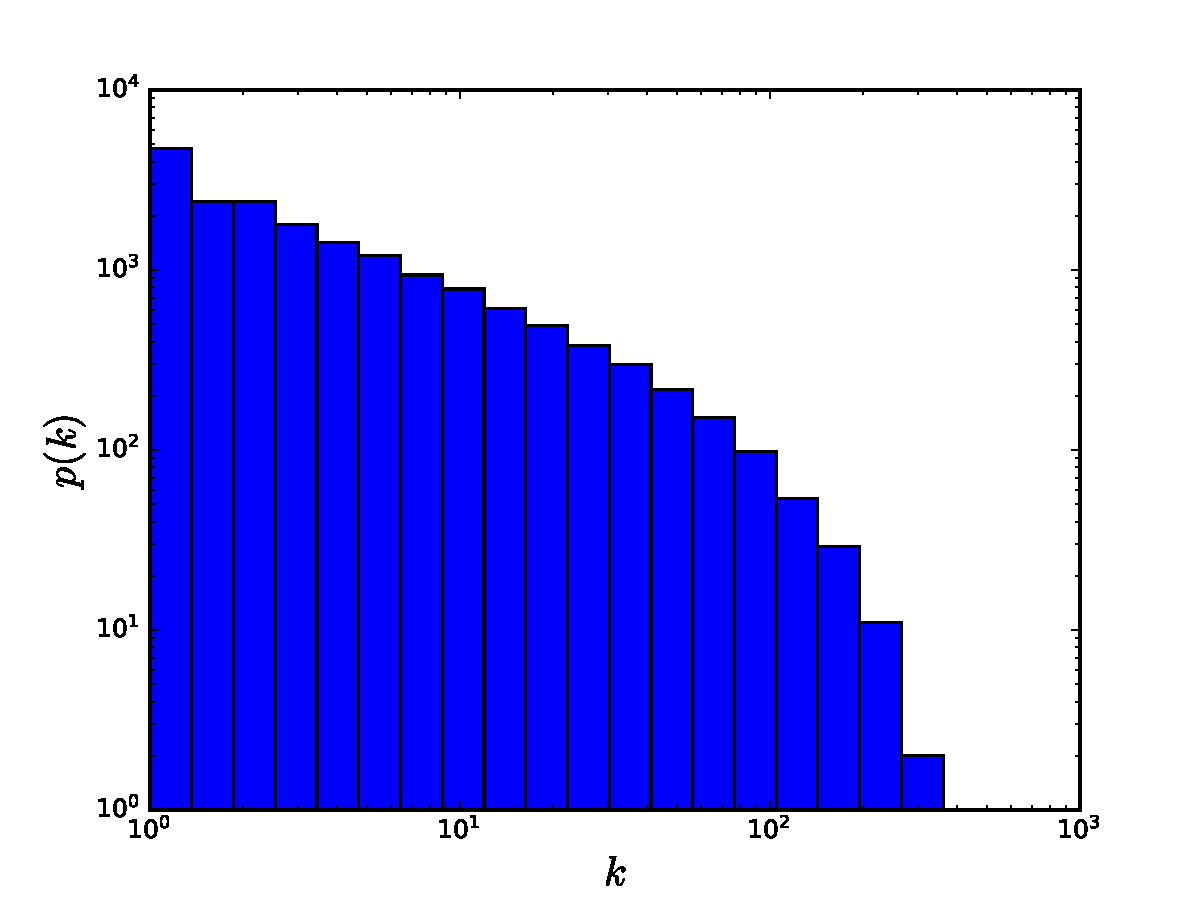
\includegraphics[width=\columnwidth]{deg_distri_global_airport_log_logbins_cumul.pdf}
%    \end{columns}
%\end{frame}
%--------------------------------------
%--------------------------------------
\begin{frame}
    \frametitle{Detecting and visualizing power-laws}
    \centering
    {\bf A portion of the internet \footnote{Taken from the website of Mark Newman}}

    \vspace{2em}
    \begin{columns}
    \column{0.35\linewidth}
        \centering
        {\bf Log-log scale}
        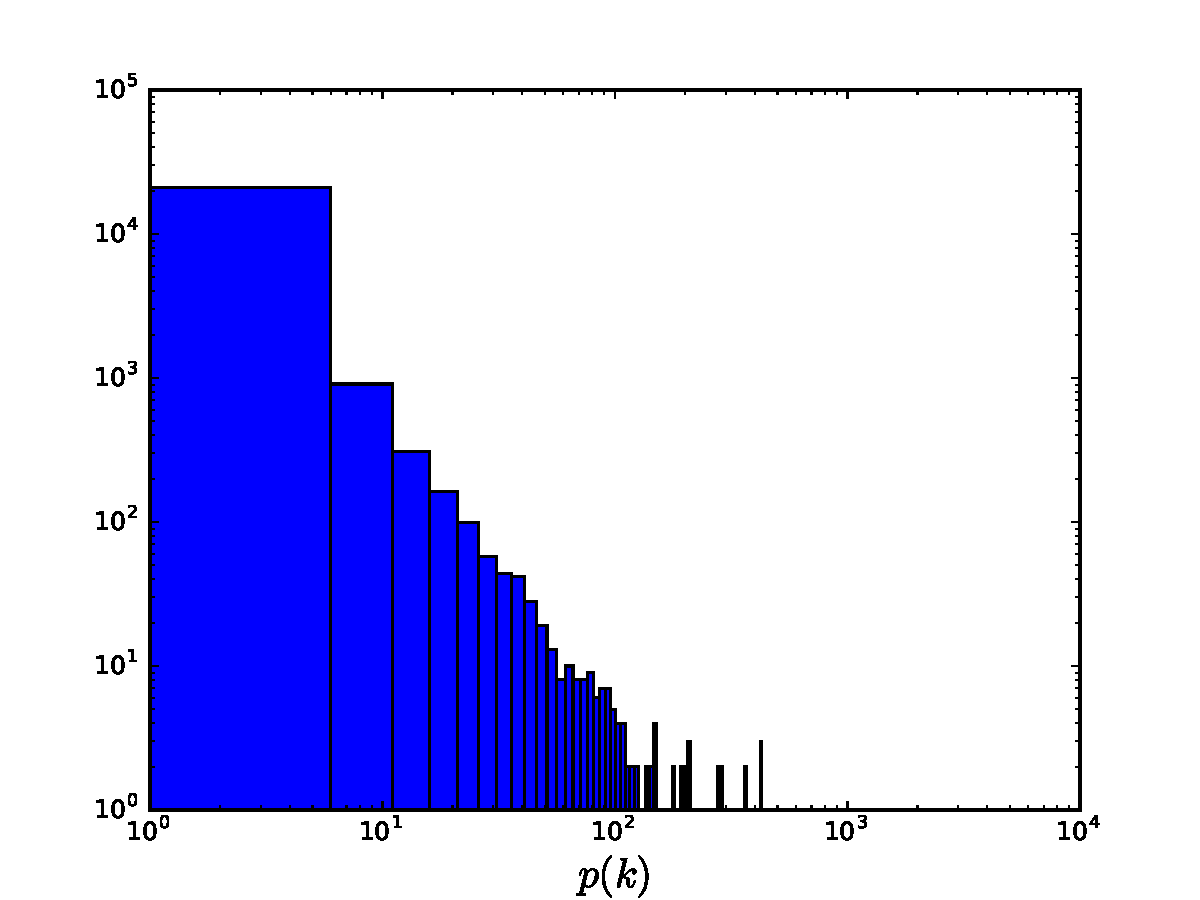
\includegraphics[width=\columnwidth]{internet_loglog_hist.pdf}
    \column{0.35\linewidth}
        \centering
        {\bf Logarthmic bins}
        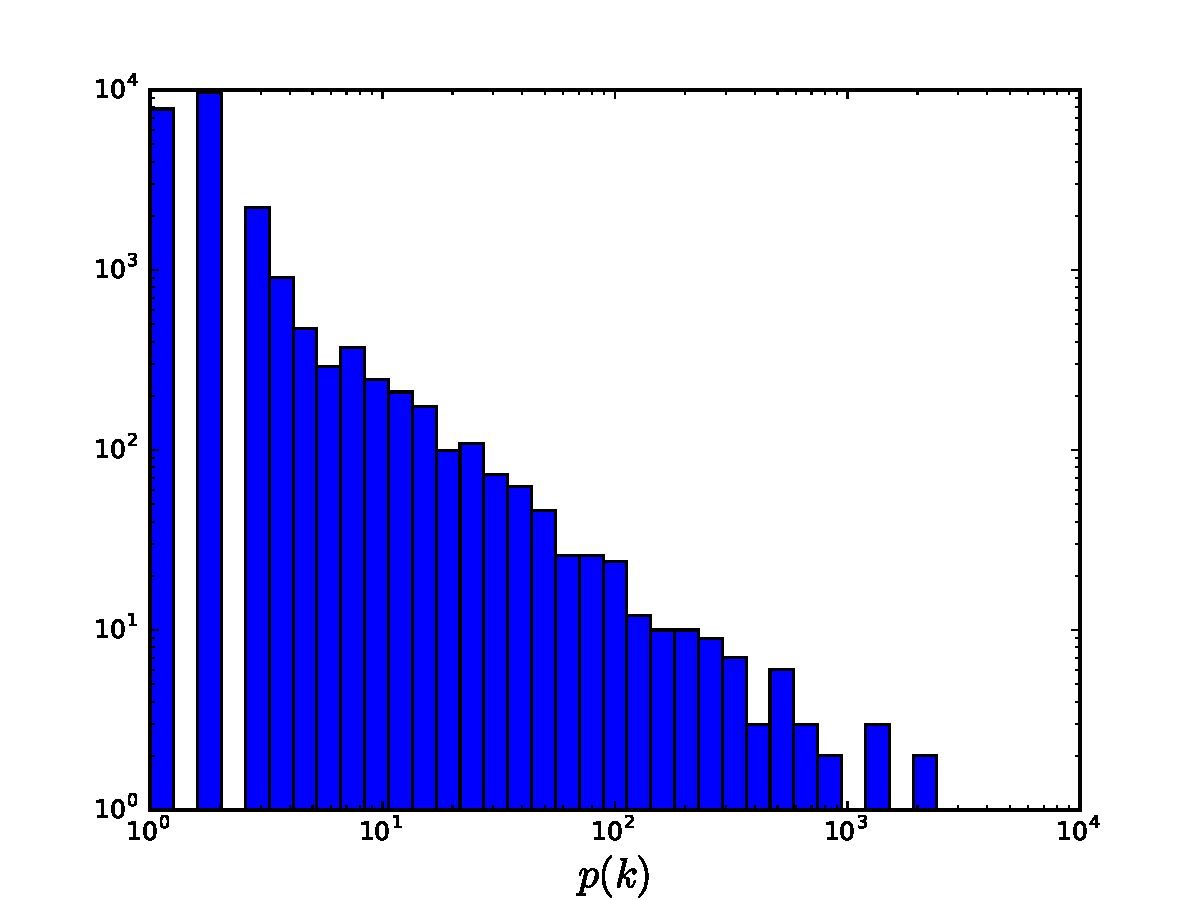
\includegraphics[width=\columnwidth]{internet_loglog_logbin_hist.pdf}
    \column{0.35\linewidth}
        \centering
        {\bf Cumulative }
        %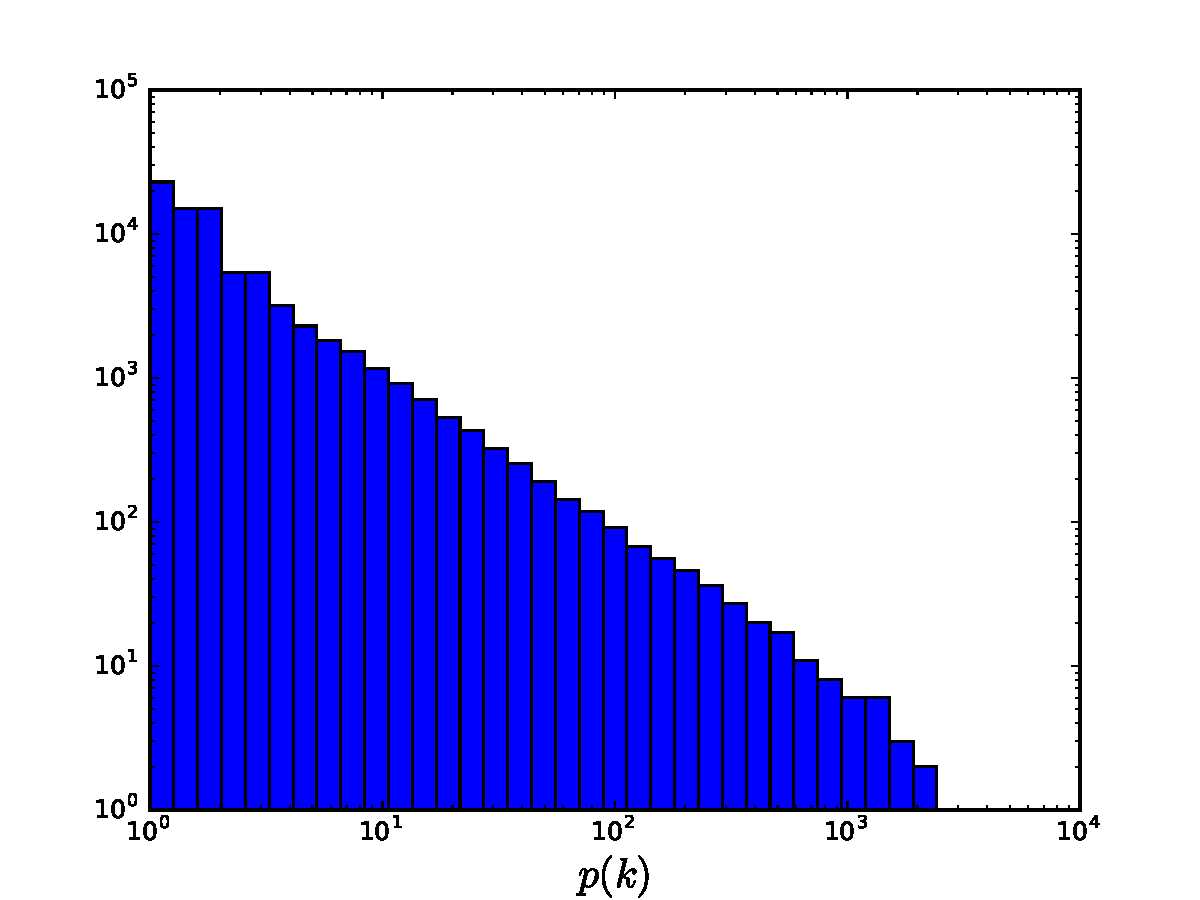
\includegraphics[width=\columnwidth]{internet_loglog_logbin_cum_hist.pdf}
        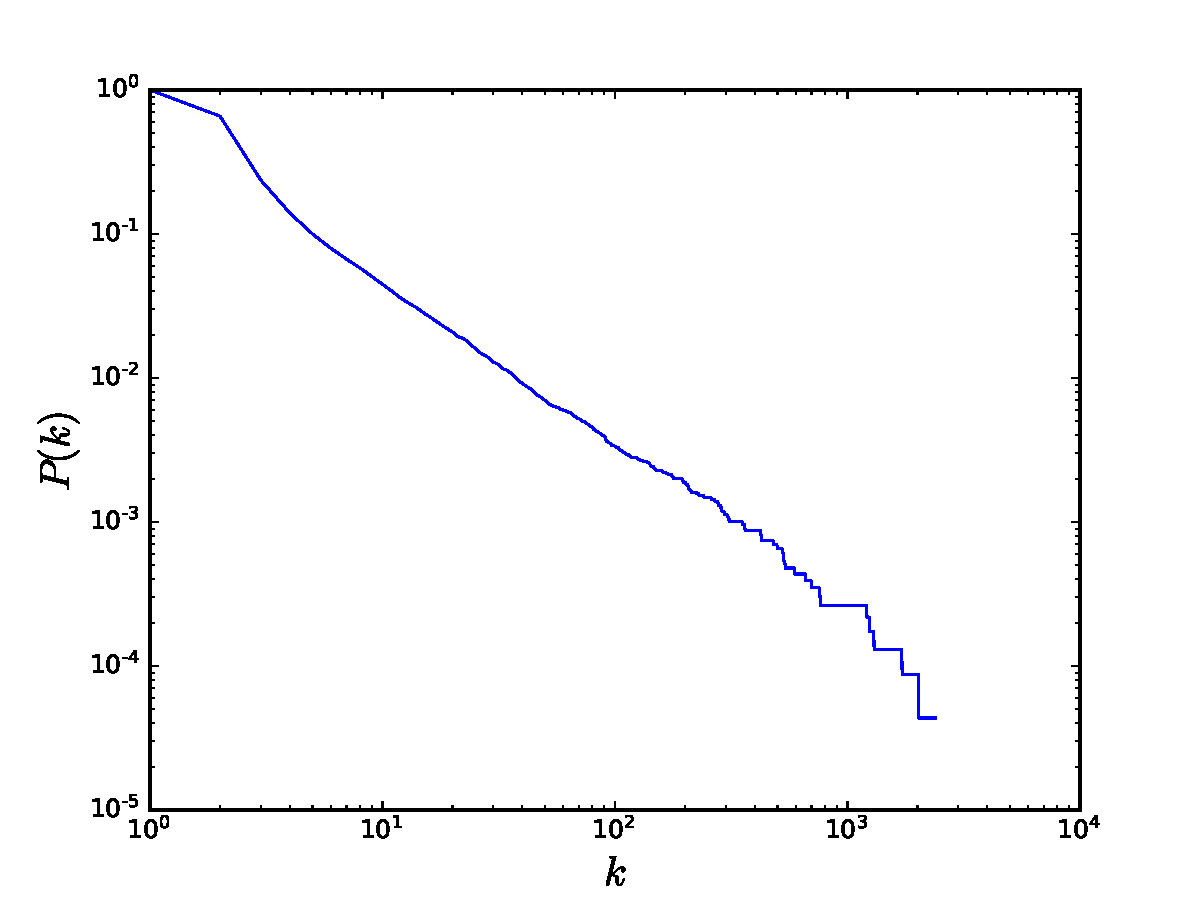
\includegraphics[width=\columnwidth]{internet_loglog_cum_hist2.pdf}
    \end{columns}
    \note{Values are not independent in cumulative distribution\\.\\Don't do fitting!}
\end{frame}
%--------------------------------------
%--------------------------------------
\begin{frame}
    \frametitle{}
    Calculation of the scaling exponent
    
    \centering
    $$\alpha = 1 + \frac{N}{\left[\sum\limits_i\frac{k_i}{k_{\text{min}}-\frac{1}{2}}\right]}$$

    \justifying
    Statistical error on $\alpha$
    $$\sigma = \frac{\alpha-1}{\sqrt{N}}$$
\end{frame}
%--------------------------------------
%--------------------------------------
\begin{frame}
    \frametitle{Assortative mixing}
    \vspace{2em}
    \centering
    {\small Social network of school-children with two races: Black and White}
    \begin{figure}
        \begin{center}
        %\includegraphics[width=0.8\columnwidth,trim=20 200 200 20,clip=true]{assortativity_high_school.pdf}
        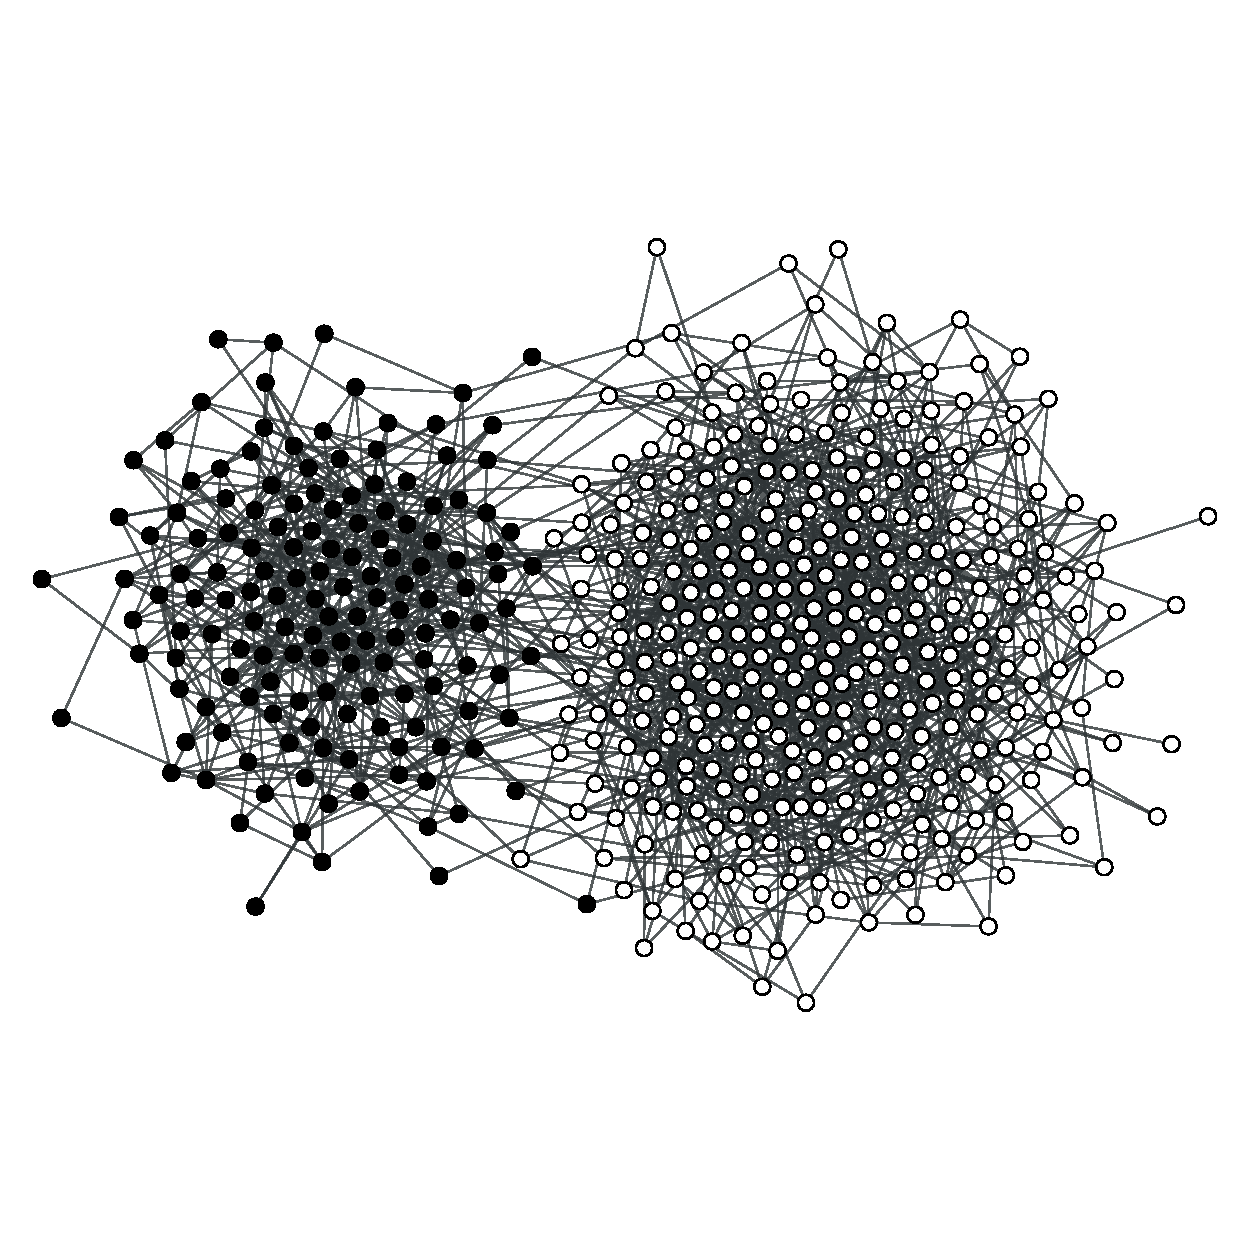
\includegraphics[width=0.8\columnwidth,trim=0 0 0 50,clip=true]{assort_network.pdf}
        \end{center}
    \end{figure}
\end{frame}
%--------------------------------------
%--------------------------------------
\begin{frame}
    \frametitle{Assortative mixing}
        \begin{itemize}
        \setlength\itemsep{1em}
            \item{{\bf Social networks:} race, age, physical locations, language, income, educational level}
            \item{{\bf Citation networks:} topics of the study}
            \item{{\bf World Wide Web:} contents of the webpages}
            \item{{\bf Internet:} physical locations}
        \end{itemize}
\end{frame}
%--------------------------------------
%--------------------------------------
\begin{frame}
    \centering
        \vspace{1em}
    {\bf Assortative mixing by enumerative characteristics}
        \begin{itemize}
        \setlength\itemsep{1em}
            \item{Characteristics with a finite set of values} 
            \item{No ordering} 
            \item{Nationality, Gender, Race} 
        \end{itemize}
        \vspace{1em}
    {\bf Assortative mixing by scalar characteristics}
        \begin{itemize}
        \setlength\itemsep{1em}
            \item{Characteristics with a finite or infinite set of values}
            \item{Ordering}
            \item{Age, income, degree}
        \end{itemize}
        \pause
        \vspace{1em}
        The network is {\bf assortative} if a large fraction of the edges fall between vertices of the same type

        \vspace{1em}
        If the opposite is true, the network is called {\bf dissortative}
\end{frame}
%--------------------------------------
%--------------------------------------
\begin{frame}
    \frametitle{Quantification for enumerative characteristics}
        
    \begin{itemize}
    \setlength\itemsep{2em}
        \item{Fraction of edges connecting vertices of the same type?}
        
        \pause
        \item{Fraction of the actual minus the expected number of edges connecting the vertices when connections are made at random\\

        \pause
        \item{Has value $0$ in trivial cases}
}
    \end{itemize}
\end{frame}
%--------------------------------------
%--------------------------------------
\begin{frame}
    \frametitle{Number of edges between the same types}
        \begin{center}
        $c_i$ : the class or type of vertex $i$\\
        \vspace{2em}
        $n_c$ : total number of types
        \vspace{2em}

        Total number of edges between the vertices of the same type:
        $$\sum\limits_{\text{edges}(i,j)}\delta(i,j)=\frac{1}{2}\sum\limits_{i,j}A_{ij}\delta(c_i,c_j)$$ 
        \end{center}
\end{frame}
%--------------------------------------
%--------------------------------------
\begin{frame}
    \frametitle{Expected number of edges between the same types}
    \begin{itemize}
    \setlength\itemsep{1em}
        \item{Half-edges or stubs, degrees preserved}
        \item{For a given stub at vertex $i$, there are $2m-1$ stubs to which it can connect to}
        \item{Probability of connecting vertex $j$ is $\frac{k_j}{2m}$}
        \item{Expected number of edges between $i$ and $j$ is $\frac{k_ik_j}{2m-1}$}
        \item{Expected number of edges between all the pairs of the same type:
            $$\frac{1}{2}\sum\limits_{ij}\frac{k_ik_j}{2m}\delta(c_i,c_j)$$
}
    \end{itemize}
\end{frame}
%--------------------------------------
%--------------------------------------
\begin{frame}
    \frametitle{Modularity}
        $$\frac{1}{2}\sum\limits_{i,j}A_{ij}\delta(c_i,c_j)-\frac{1}{2}\sum\limits_{ij}\frac{k_ik_j}{2m}\delta(c_i,c_j)=\frac{1}{2}\sum\limits_{ij}\left(A_{ij}-\frac{k_ik_j}{2m}\right)\delta(c_i,c_j)$$ 

        \vspace{2em}
        \pause
        $$Q = \frac{1}{2m}\sum\limits_{ij}\left(A_{ij}-\frac{k_ik_j}{2m}\right)\delta(c_i,c_j)$$

        \vspace{2em}
        \centering
        $Q$ is called the {\bf modularity} of the network w.r.t. to $c$

        $$B_{ij}=A_{ij}-\frac{k_ik_j}{2m}$$
\end{frame}
%--------------------------------------
%--------------------------------------
\begin{frame}
    \frametitle{Normalized modularity}
    \centering
    Modularity is not $1$ even for a perfectly mixed network.

    \pause

    $$Q_{\text{max}} = \frac{1}{2m}\left(2m-\sum\limits_{ij}\frac{k_ik_j}{2m}\delta(c_i,c_j)\right)$$

    \pause
    $$Q_{\text{norm}} = \frac{Q}{Q_{\text{max}}}$$
\end{frame}
%--------------------------------------
%--------------------------------------
\begin{frame}
    \frametitle{Quantification for scalar characteristics}
    \centering
    $x_i$ : a scalar value for vertex $i$
    \vspace{1em}

    $$r = \frac{\sum\limits_{ij}(A_{ij}-k_ik_j/2m)x_ix_j}{\sum\limits_{ij}(k_i\delta_{ij}-k_ik_j/2m)x_ix_j}$$
\end{frame}
%--------------------------------------
%--------------------------------------
\begin{frame}
    \frametitle{Degree-correlations/Degree-assortativity}
    
    \begin{itemize}
    \setlength\itemsep{1em}
        \item{Using degree itself as a scalar property of the nodes}
        \item{Degree is the property of the network structure}
        \item{One property (degree) dictating the others (position of the edges)}
    \end{itemize}
\end{frame}
%--------------------------------------
%--------------------------------------
\begin{frame}
    \frametitle{}
    \centering
    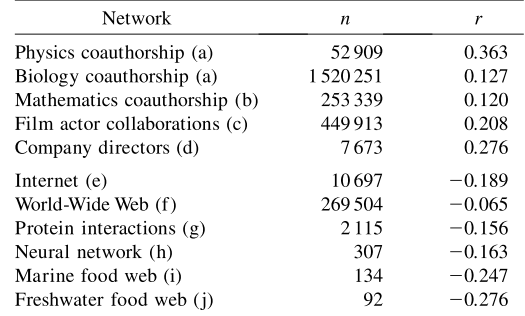
\includegraphics[width=\columnwidth]{assortativity_list.png}
\footnote{Newman, M.E.J., Assortative Mixing in Networks, PRL, 89, 20.}
\end{frame}
%--------------------------------------
%--------------------------------------
\begin{frame}
    \frametitle{Random graph models}
    \centering

    \begin{itemize}
    \setlength\itemsep{1em}
        \item{Generative models of networks}
        \item{Probabilistic models capable of generating an observed data}
        \item{Certain properties can be fixed for generative models}
        \item{Better way to describe the structure of the networks}
    \end{itemize}
        
\end{frame}
%--------------------------------------
%-------------------------
\begin{frame}
    \frametitle{}
    \begin{columns}
    \column{0.6\linewidth} 
    \centering
    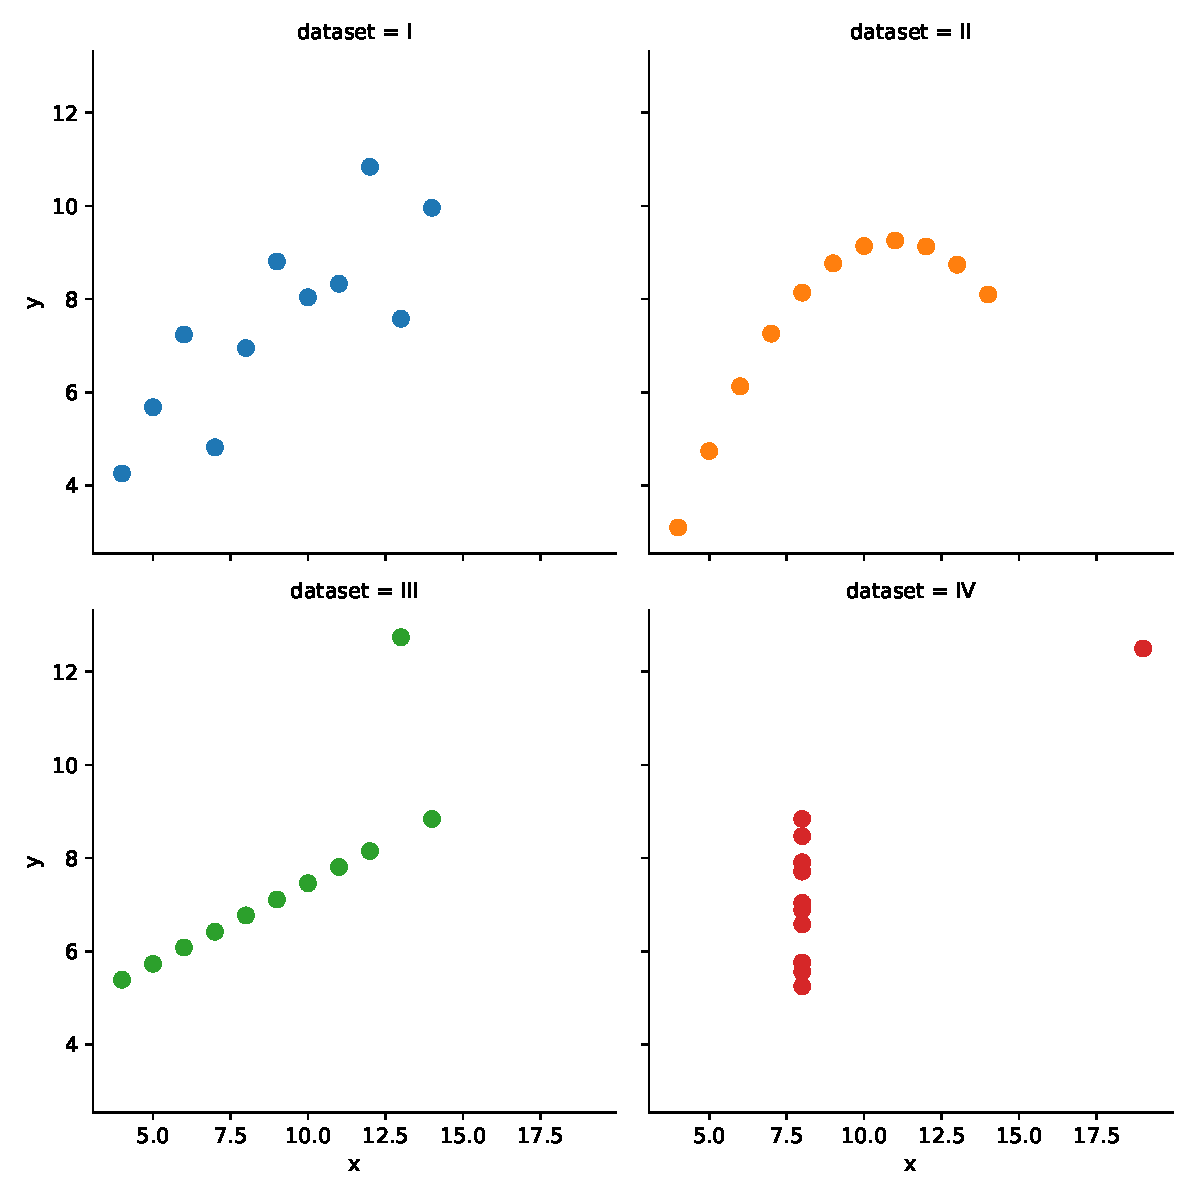
\includegraphics[width=\columnwidth]{anscombe.pdf} 
    \column{0.6\linewidth} 
    
    \pause
    \begin{itemize}
    \setlength\itemsep{1em}
        \item{Mean of $x = 9$}
        \item{Variance of $x = 11$}
        \item{Mean of $y = 7.5$}
        \item{Variance of $y = 4.125$}
        \item{Correlation = $0.816$}
    \end{itemize}
    \end{columns}
    \centering
    \vspace{2em}
    {\bf Anscombe's quartet!}
\end{frame}
%-------------------------
%-------------------------
\begin{frame}
    \frametitle{Random graph models (RGMs)}
    \centering
    \begin{itemize}
    \setlength\itemsep{1em}
        \item{\textcolor{red}{Erd{\H o}s-R{\'e}nyi model}}
        \item{\textcolor{red}{Configuration model}}
        \item{Stochastic-block model}
        \item{Degree-corrected SBM}
        \item{Equitable random graphs}
        \item{Hierarchical block models}
        \item{Random graphs with expected degrees}
        \item{Microcanonical SBM}
        \item{Poisson SBM}
    \end{itemize}
\end{frame}
%-------------------------
%-------------------------
\begin{frame}
    \frametitle{Erd{\H o}s-R{\'e}nyi model (ER model/$G(n, p)$)}
    \begin{itemize}
    \setlength\itemsep{1em}
        \item{Fix $n$ and the average degree $c$}
        \item{Connect every pair of nodes with a probability $p = \frac{c}{n-1}$}
        \item{Number of graphs in the ensemble: $2^{\binom{n}{2}}$}
        \item{ER model: Every member of the ensemble is equally likely}
    \end{itemize}
    \note{Uniform probability distribution over the ensemble}
    \centering
        \centering
            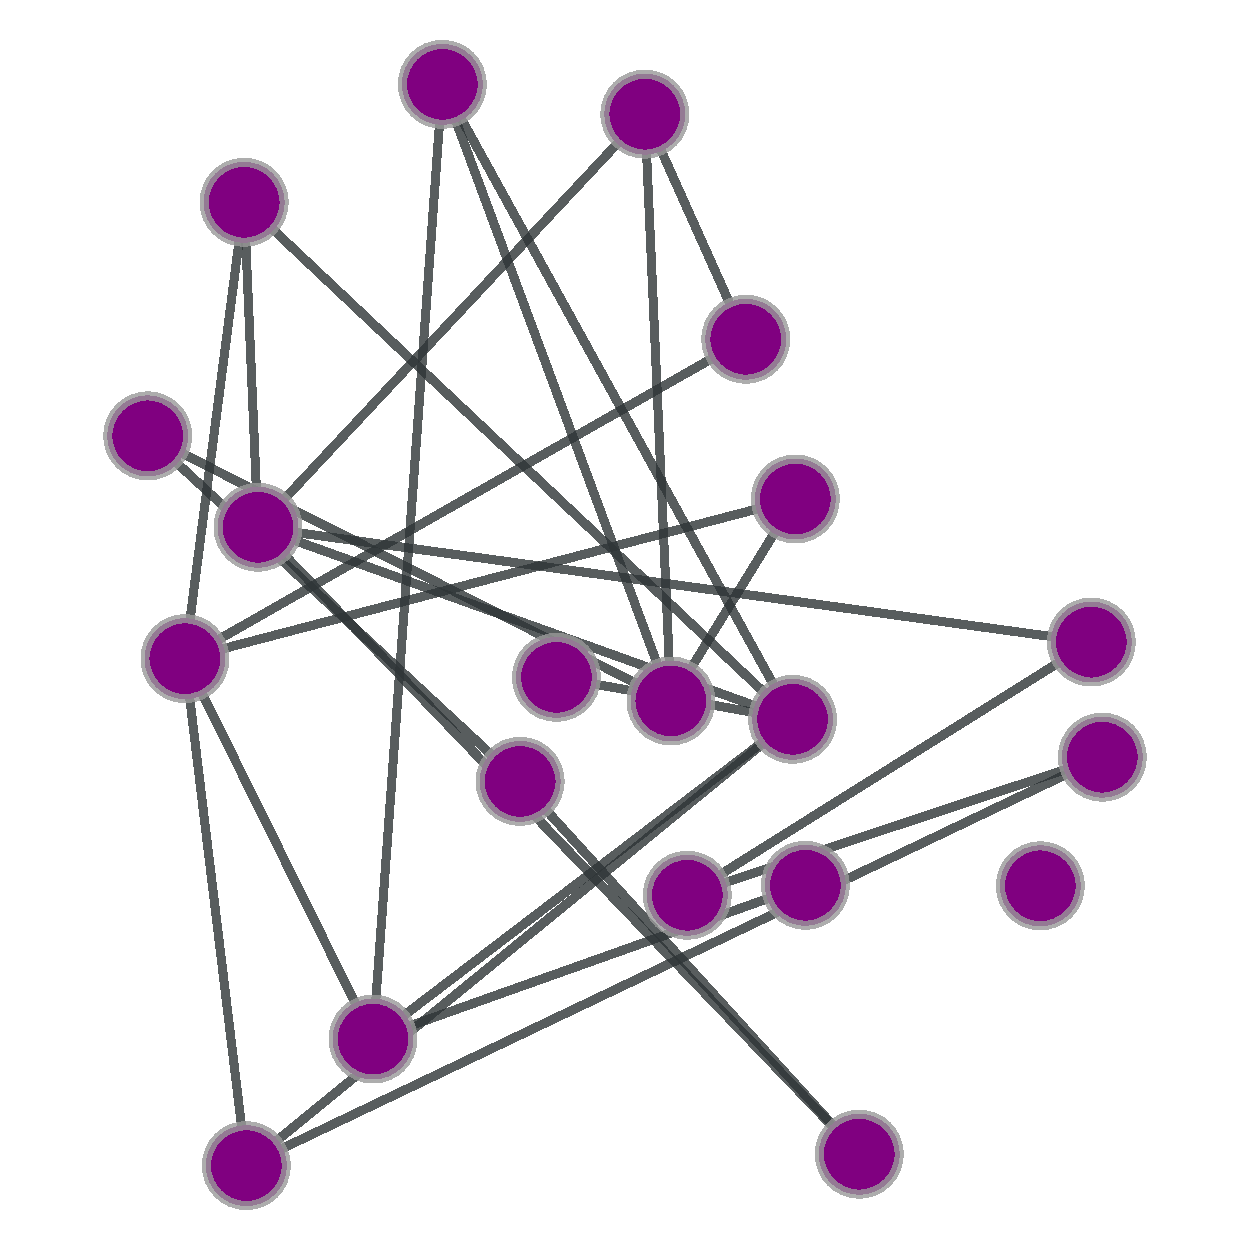
\includegraphics[width=0.3\columnwidth]{er0.pdf}
            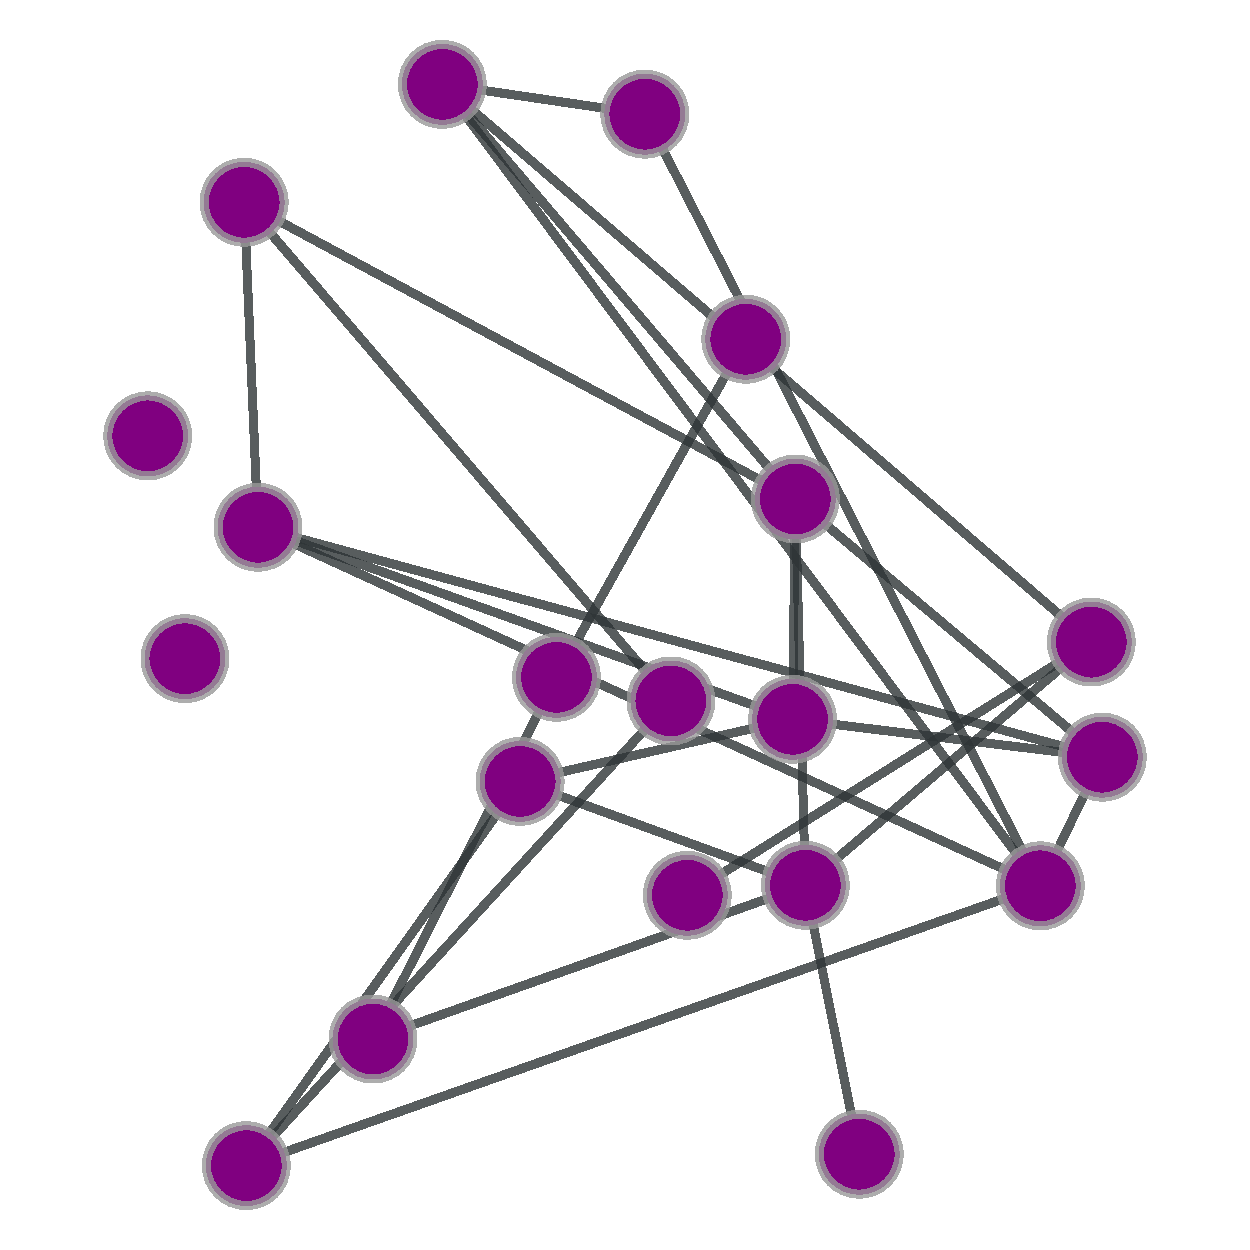
\includegraphics[width=0.3\columnwidth]{er1.pdf}
            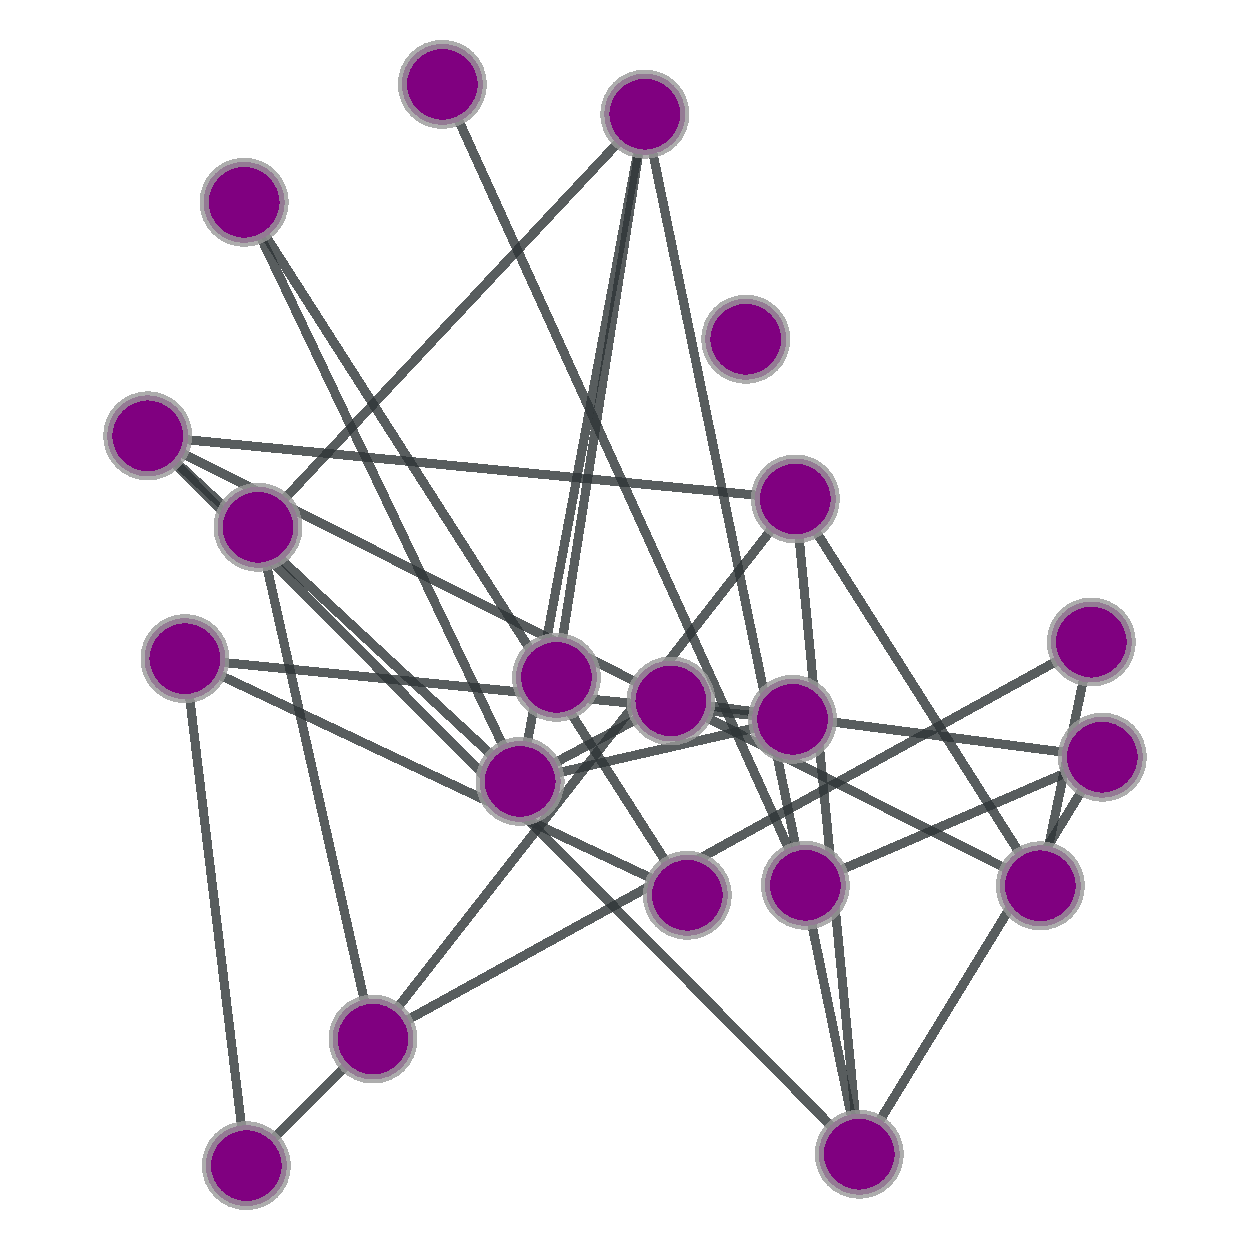
\includegraphics[width=0.3\columnwidth]{er2.pdf}
\end{frame}
%-------------------------
%-------------------------
\begin{frame}
    \frametitle{Properties of the ER model}
    \centering
    {\bf Average properties of the ensemble}
    $$<m> = \sum\limits_GP(G)m(G) = \frac{1}{\Omega}\sum\limits_Gm(G)$$
\end{frame}
%-------------------------
%-------------------------
\begin{frame}
    \frametitle{Properties of the ER model}
    \centering
    {\bf Degree distribution}
    
    \vspace{2em}
    \begin{itemize}
        \setlength\itemsep{1em}
        \item{Given vertex can connect to remaining $n-1$ vertices}
        \item{Probability of connecting to particular $k$ vertices: $$p^k(1-p)^{n-1-k}$$}
        \item{There are $\binom{n-1}{k}$ ways to choose $k$ vertices}
    \end{itemize}
    \vspace{1em}
    $p_k = \binom{n-1}{k}p^k(1-p)^{n-1-k} = e^{-c}\frac{c^k}{k!}$
    \note{Poisson distribution with mean $c$//.//Poisson random graph//.//$$\lim\limits_{n\to\infty}\left(1+\frac{a}{n}\right)^n = e^a$$}
\end{frame}
%-------------------------
%-------------------------
%\begin{frame}
%    \frametitle{}
%    $$p_k = \binom{n-1}{k}p^k(1-p)^{n-1-k}$$
%    $$\therefore p_k = \binom{n-1}{k}\left(\frac{c}{n-1}\right)^k\left(1-\frac{c}{n-1}\right)^{n-1-k} = e^{-c}$$
%    \centering
%\end{frame}
%-------------------------
%-------------------------
\begin{frame}
    \frametitle{The giant component}
    \centering
    $$p = 0 \hspace{10em} p = 1$$
    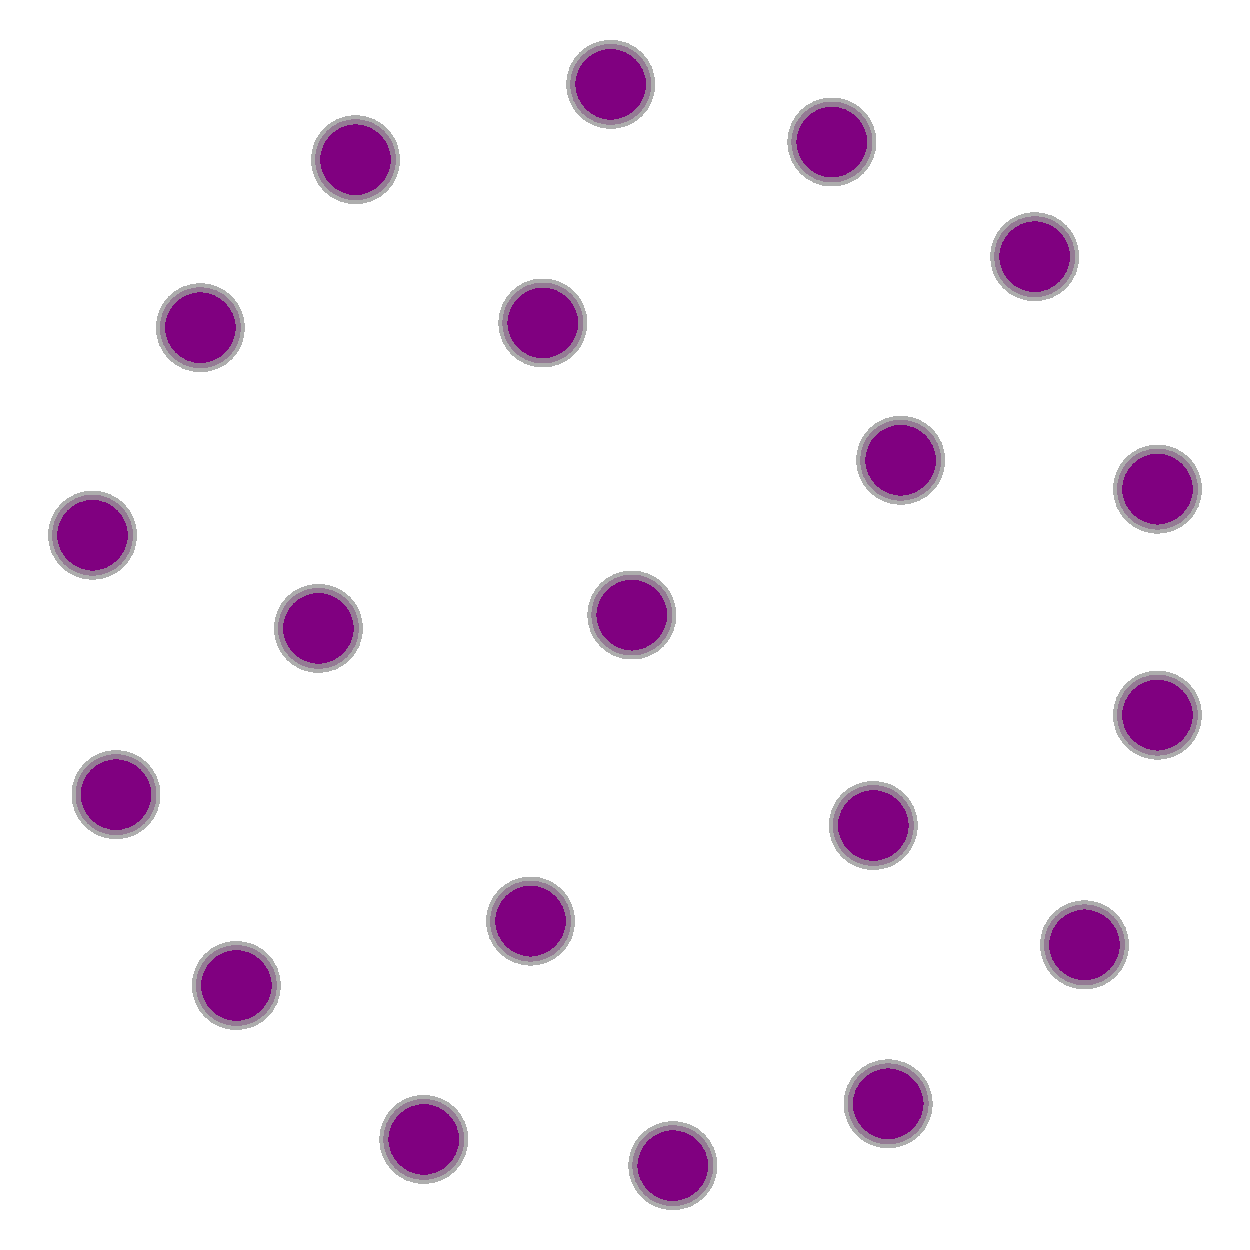
\includegraphics[width=0.4\columnwidth]{er3.pdf}
    \hspace{2em}
    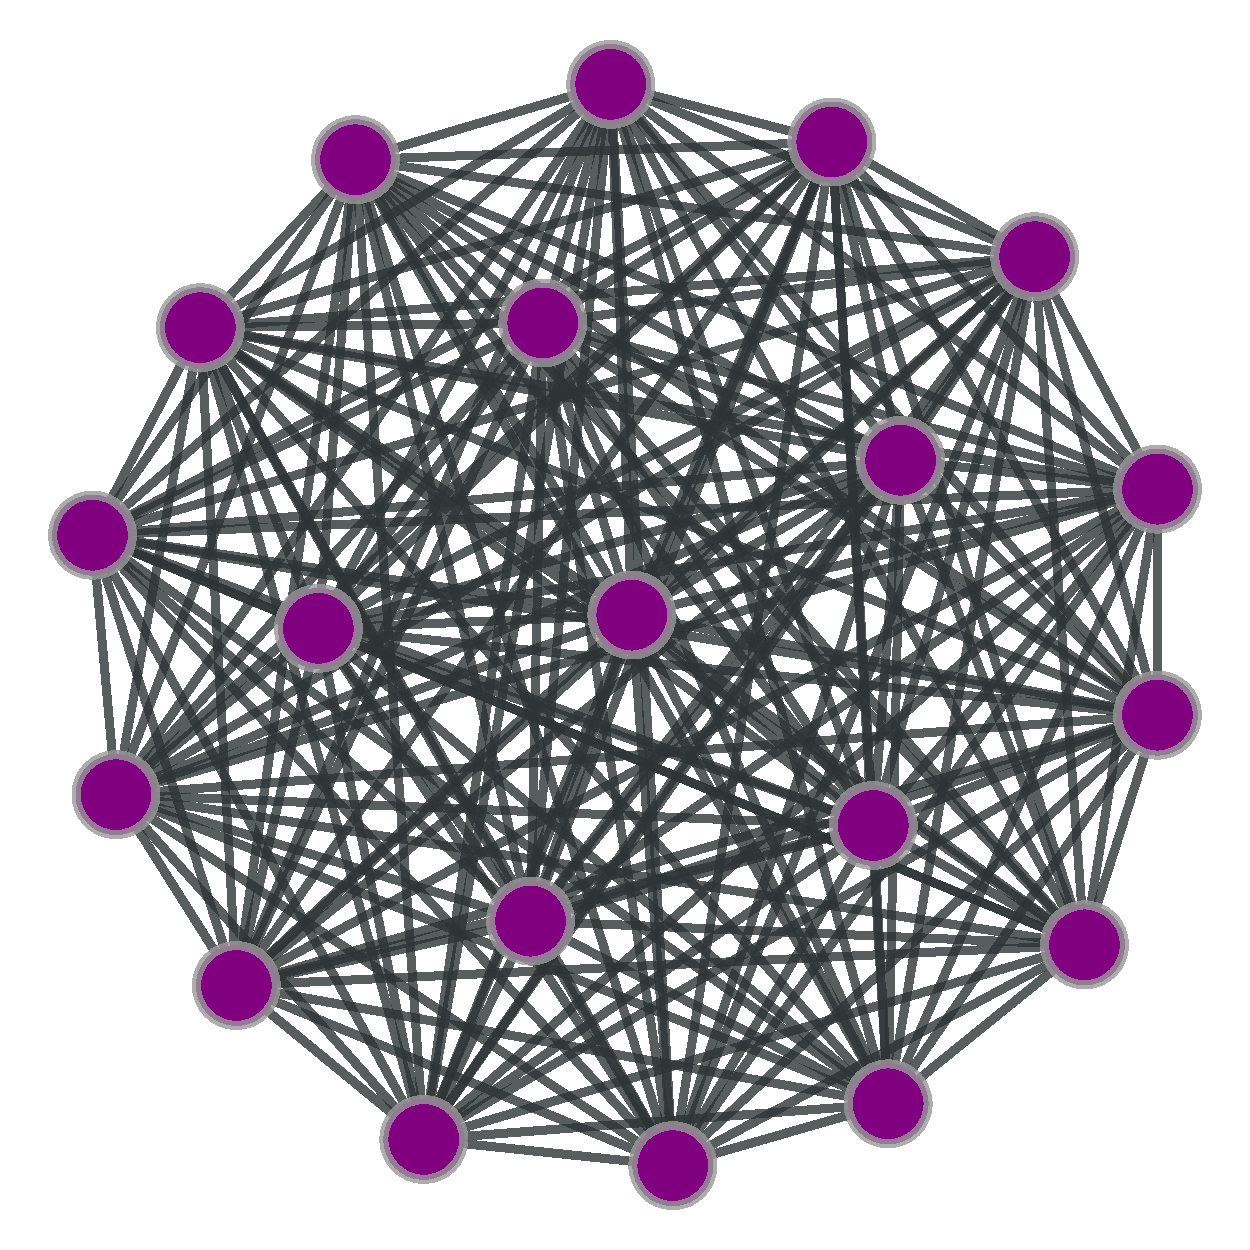
\includegraphics[width=0.4\columnwidth]{er4.pdf}

    \vspace{1em}
    {\bf What is the size of the largest component?}
\end{frame}
%-------------------------
%-------------------------
\begin{frame}
    \frametitle{The giant component}
    \centering
    \begin{itemize}
        \setlength\itemsep{1em}
        \item{Giant component: size is an extensive function of the network size}
        \item{Transition between the two extremes with $p$: gradual or sudden?}
        \item{Size of the giant component as a function of $p$ can be calculated exactly in the limit}
    \end{itemize}
\end{frame}
%-------------------------
%-------------------------
\begin{frame}
    \frametitle{The giant component}
    %\centering
    $u$ : Fraction of vertices not in the giant component\\

    \note{$u = 1$ when no giant component}
    \justifying
    \vspace{1em}
    When is a vertex $i$ not in the giant component?\\

    \vspace{1em}
    For any other vertex $j$:
    \begin{enumerate}
        \setlength\itemsep{1em}
        \item{$i$ is not connected to $j$}
        \item{$i$ is connected to $j$ but $j$ is not in the giant component}
    \end{enumerate}
\end{frame}
%-------------------------
%-------------------------
\begin{frame}
    \frametitle{The giant component}
    %\centering
    $u$ : Fraction of vertices not in the giant component\\

    \note{$u = 1$ when no giant component}
    \justifying
    \vspace{1em}
    When is a vertex $i$ not in the giant component?\\

    \vspace{1em}
    For any other vertex $j$:
    \begin{enumerate}
        \setlength\itemsep{1em}
        \item{$i$ is not connected to $j$ \quad{\bf $\Rightarrow$ probability $=1-p$}}
        \item{$i$ is connected to $j$ but $j$ is not in the giant component \\{\bf $\Rightarrow$ probability $=pu$}}
    \end{enumerate}
    \vspace{1em}
    Thus, the probability of not being connected to the giant component through vertex $j$ is $(1-p+pu)$
\end{frame}
%-------------------------
%-------------------------
\begin{frame}
    \frametitle{}
    \justifying
    $$u = (1-p+pu)^{n-1}$$
    \vspace{0.5em}
    $$u = \left(1-\frac{c}{n-1}+p\frac{c}{n-1}\right)^{n-1} = \left[1-\frac{c}{n-1}(1-u)\right]^{n-1}$$
    \vspace{0.5em}
    $$u = e^{-c(1-u)}$$
    \vspace{0.5em}
    Let $S$ be the size of the giant component
    \vspace{0.5em}
    $$\therefore 1-S = e^{-cS}$$
\end{frame}
%-------------------------
%-------------------------
\begin{frame}
    \frametitle{Graphical solution for the giant component}
    \centering
    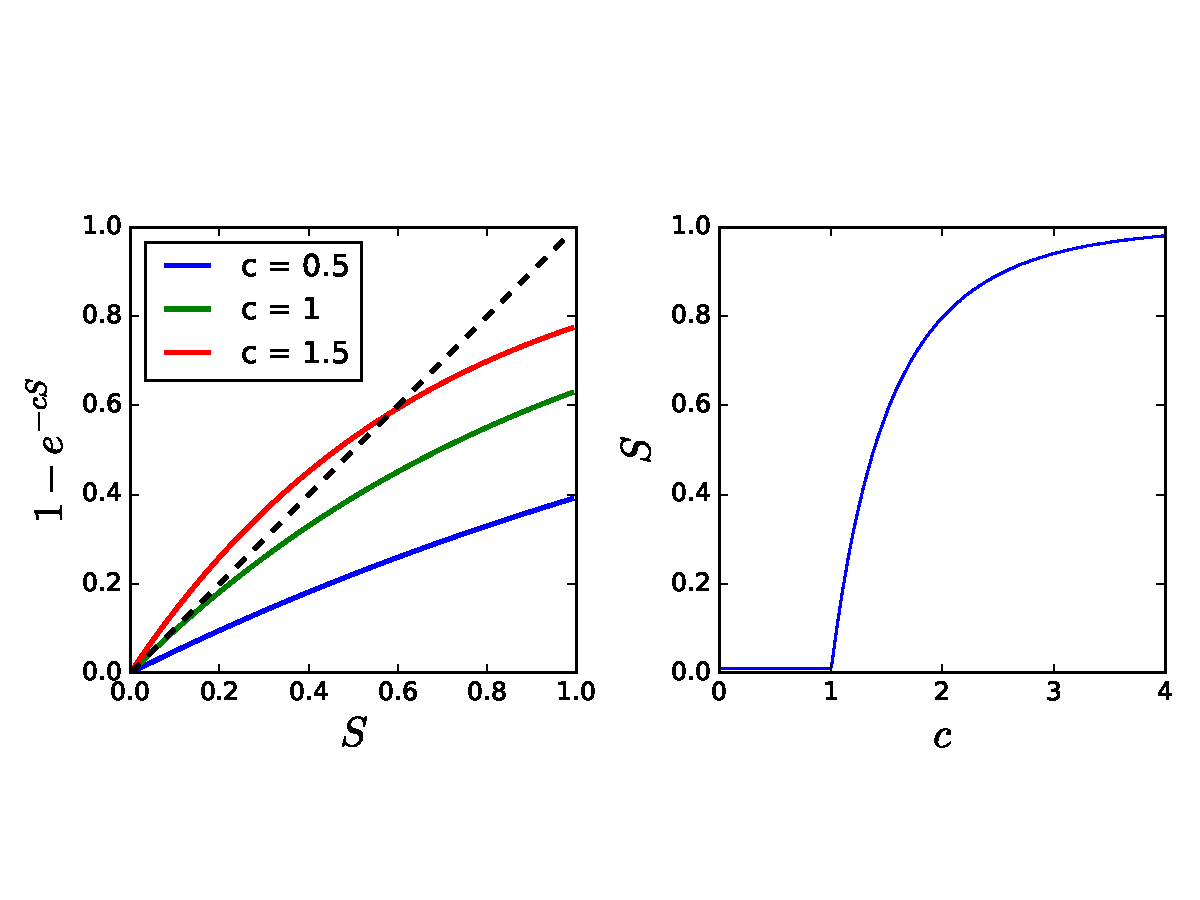
\includegraphics[width=\columnwidth]{giant_component.pdf}
    \note{One still has to prove that the giant component does exist}
\end{frame}
%-------------------------
%-------------------------
\begin{frame}
    \frametitle{}
    \centering
%\begin{equation*}
%\begin{align*}
$$\frac{d}{dS}(1-e^{-cS})\Bigr|_{S = 0} = 1$$
\vspace{2em}
$$\therefore ce^{-cS}\Bigr|_{S = 0} = 1$$
\vspace{2em}
$$\therefore c = 1$$
%\end{align*}
%\end{equation}

\end{frame}
%-------------------------
%-------------------------
\begin{frame}
    \frametitle{}
    \centering
    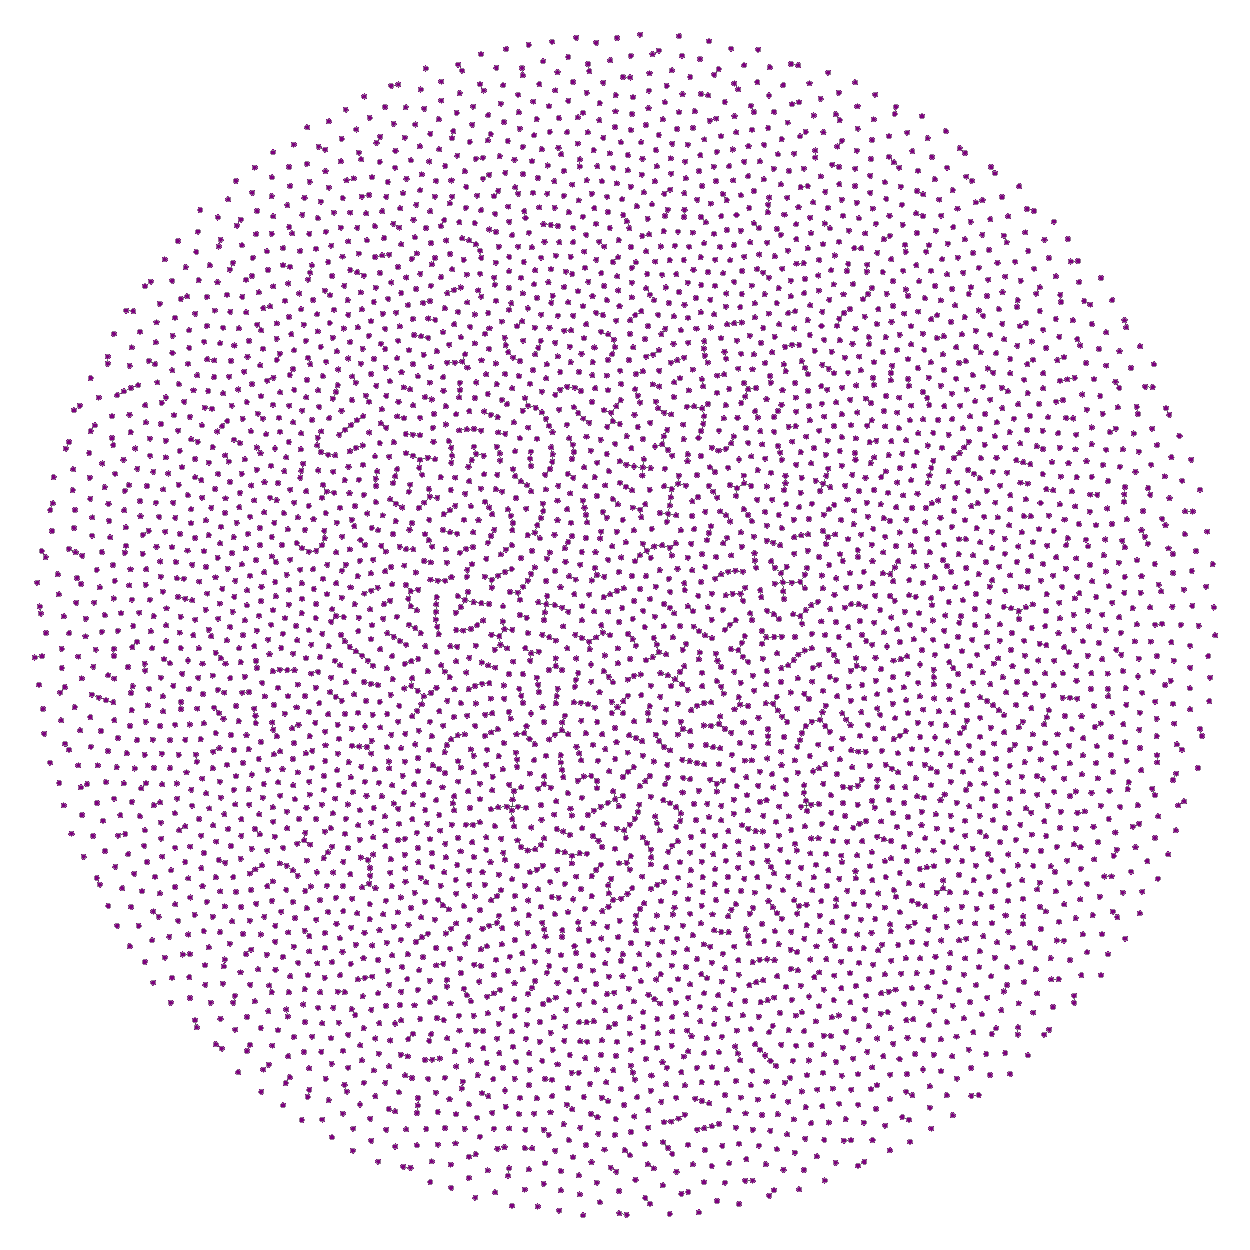
\includegraphics[width=0.55\columnwidth]{er_below_percolation.pdf}
    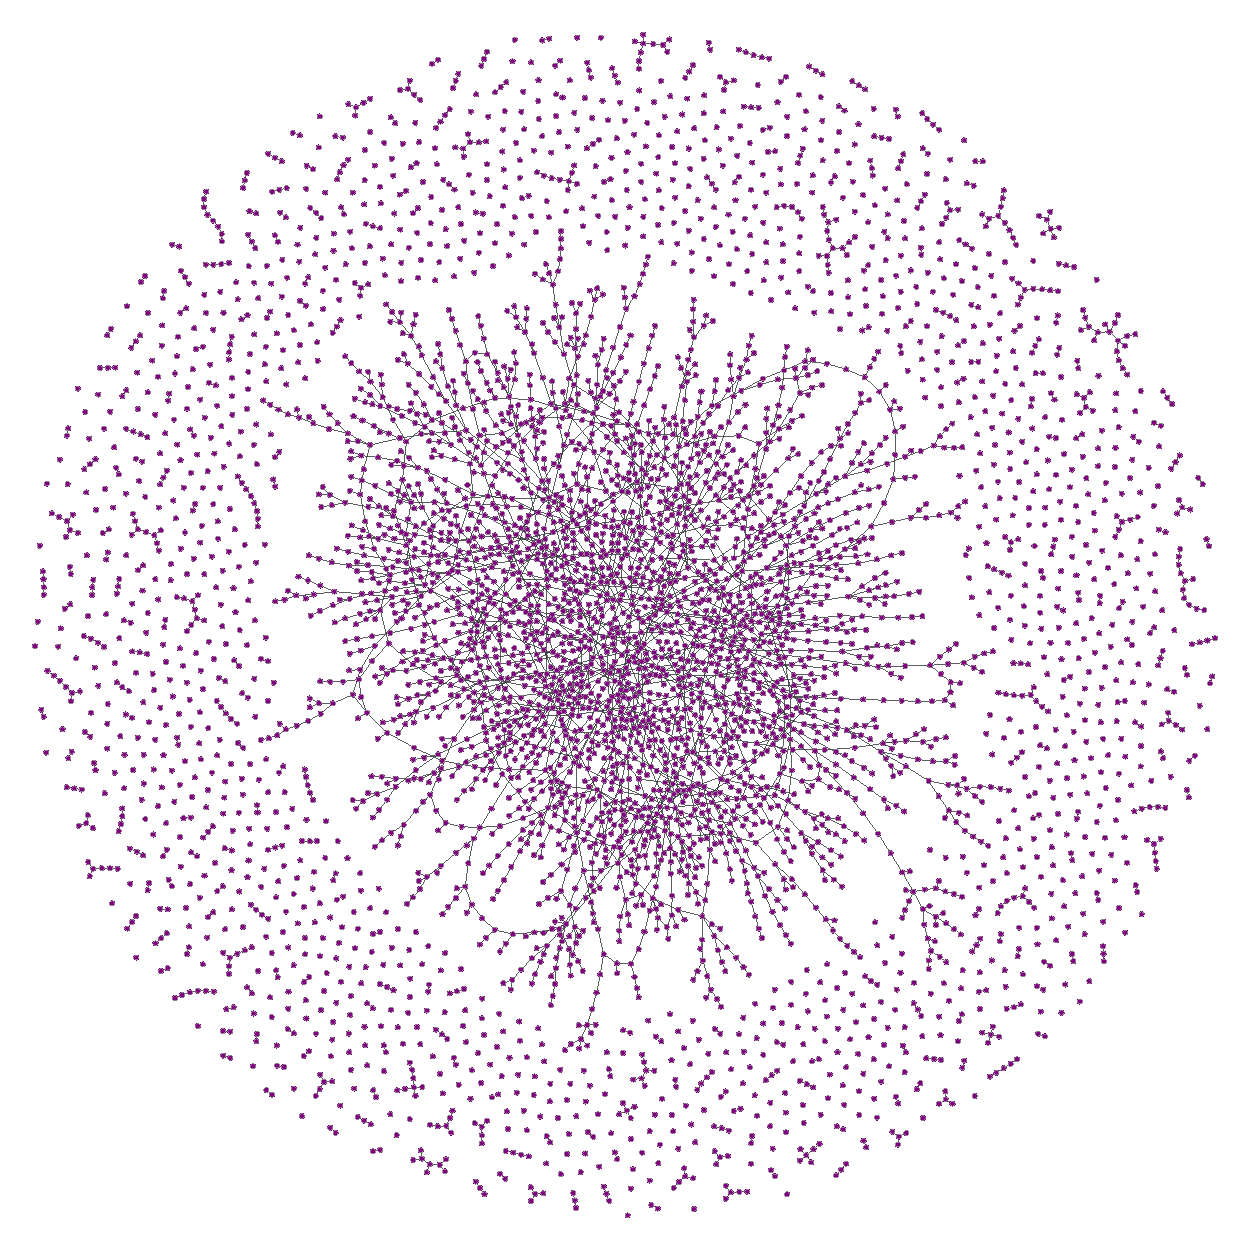
\includegraphics[width=0.55\columnwidth]{er_large.pdf}
\end{frame}
%-------------------------
%-------------------------
\begin{frame}
    \frametitle{Small components}

    \note{
    \begin{itemize}
        \setlength\itemsep{1em}
        \item{Since $S < 1$, there exist other components in the network}
        \item{Average size of the small components is intensive function of $n$}
    \end{itemize}
}
    \centering
        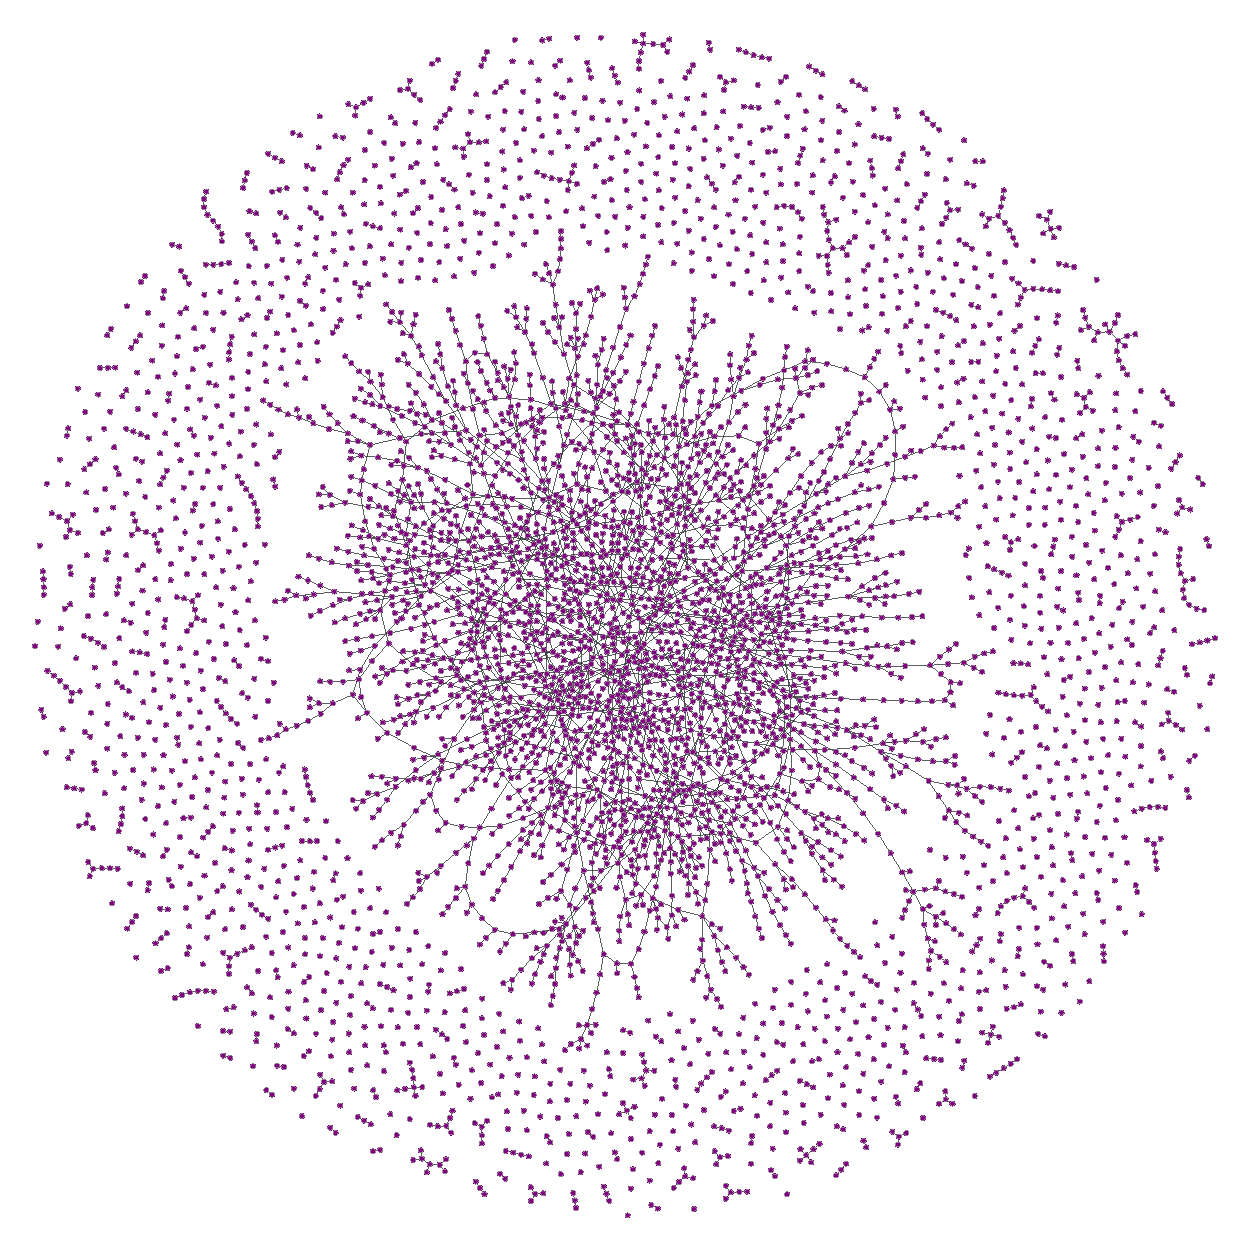
\includegraphics[width=0.8\columnwidth]{er_large.pdf}
\end{frame}
%-------------------------
%-------------------------
\begin{frame}
    \frametitle{Small components}
    \centering
    {\bf Two giant components?}\\
    \justifying
    \vspace{2em}
    %$S_1n$ and $S_2n$\\

    Distinct pairs $(i, j)$ with $i$ in $S_1$ and $j$ in $S_2$ : $S_1n\times S_2n = S_1S_2n^2$\\
    \vspace{2em}
    Probability that there is no edge between the two:
    $$q = (1-p)^{S_1S_2n^2} = \left(1-\frac{c}{n-1}\right)^{S_1S_2n^2} \sim e^{-cS_1S_2n}$$
    \note{There must be non-giant components!}
\end{frame}
%-------------------------
%-------------------------
\begin{frame}
    \frametitle{Sizes of the small components}
    \centering
    $\pi_s$ : probability that a randomly chosen vertex belongs to component of size $s$\\
    \vspace{2em}
    $$\sum\limits_{s=1}^{\infty} = 1-S$$

    \vspace{2em}
    {\bf Small-components are trees!}
\end{frame}
%-------------------------
%-------------------------
\begin{frame}
    \frametitle{Tree graph}
    \begin{columns}
        \column{0.6\linewidth}
    \centering
        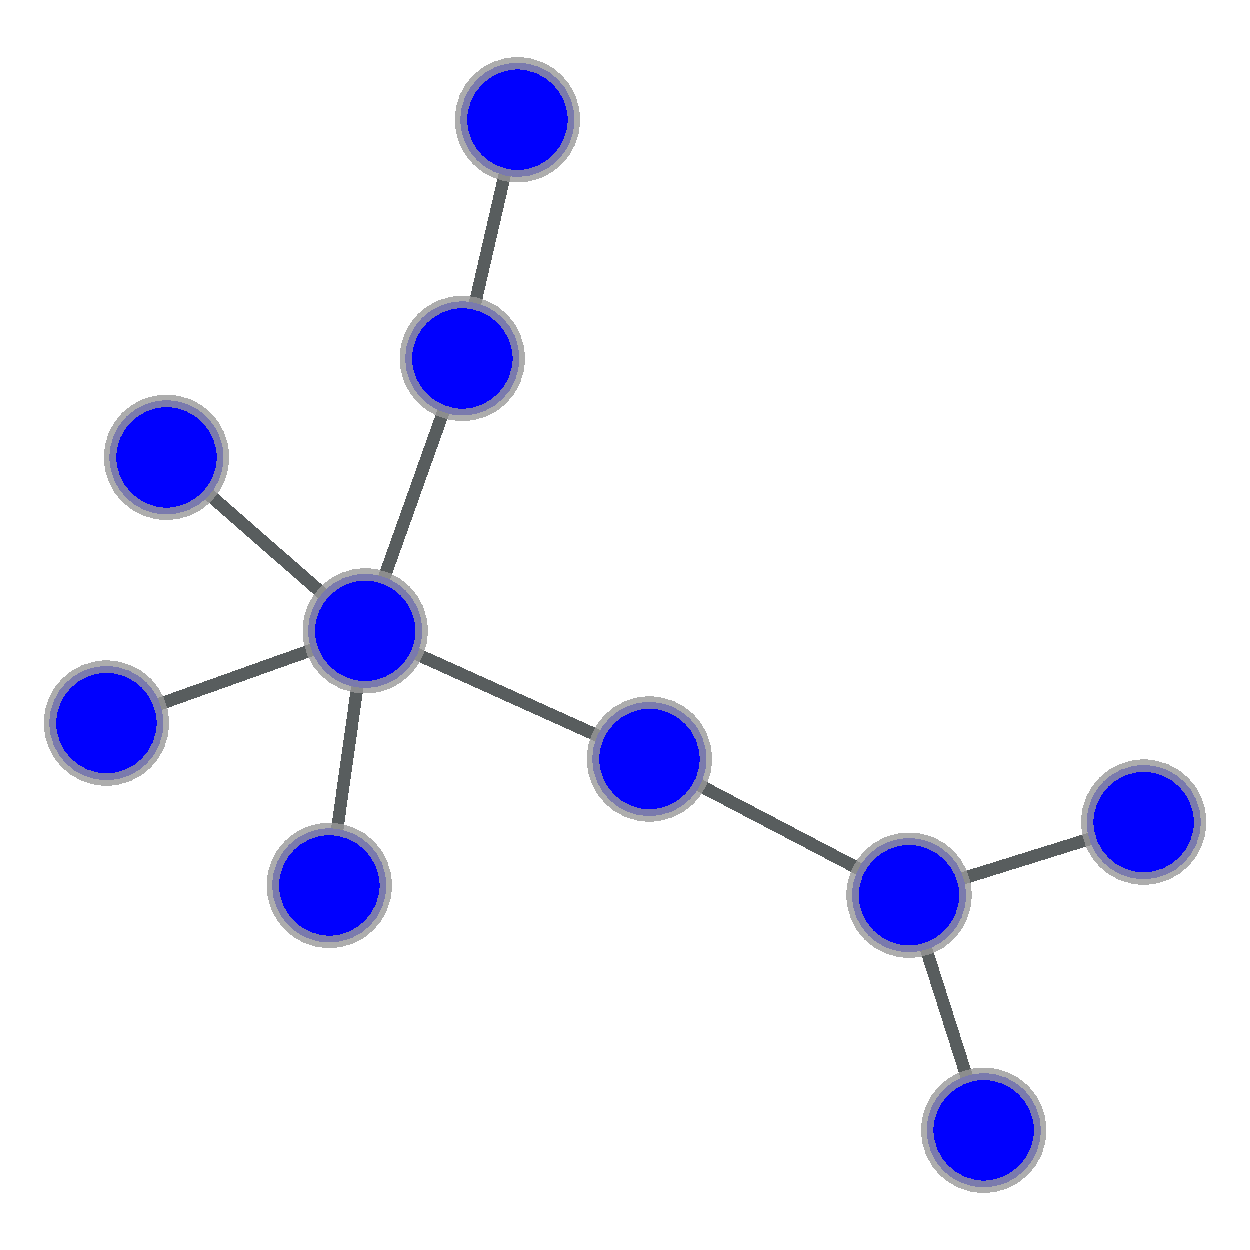
\includegraphics[width=0.8\columnwidth]{tree.pdf}
        \column{0.6\linewidth}
    \centering
    \begin{itemize}
        \setlength\itemsep{1em}
        \item{A graph without loops}
        \item{$n$ vertices and $n-1$ edges}
        \item{Removal of any vertex or edge witll disconnect the graph}
    \end{itemize}
    
    
    \end{columns}
\end{frame}
%-------------------------
%-------------------------
\begin{frame}
    \frametitle{}
    \centering
        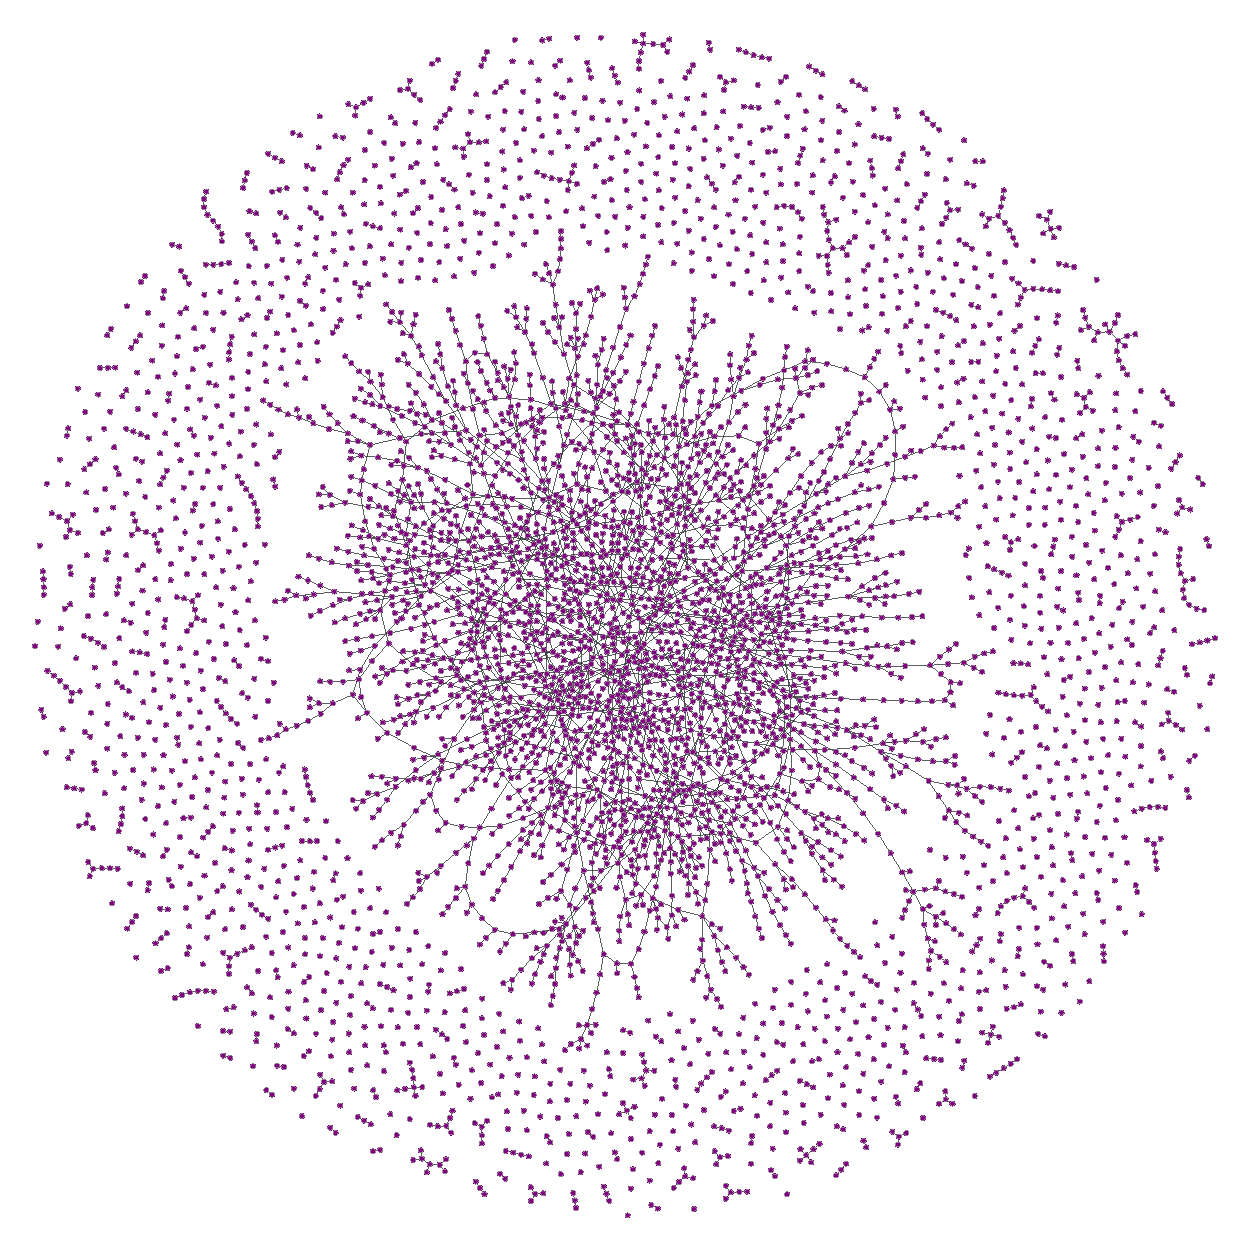
\includegraphics[width=0.8\columnwidth]{er_large.pdf}
\end{frame}
%-------------------------
%-------------------------
\begin{frame}
    \frametitle{Small components}
    \centering
    {\bf Small components are trees}
    \vspace{2em}
    $$\binom{s}{2}-(s-1) = \frac{1}{2}(s-1)(s-2)$$
    The total number of extra edges:

    $$\frac{1}{2}(s-1)(s-2)\frac{c}{n-1} \rightarrow 0$$
\end{frame}
%-------------------------
%-------------------------
\begin{frame}
    \frametitle{}
    \centering
    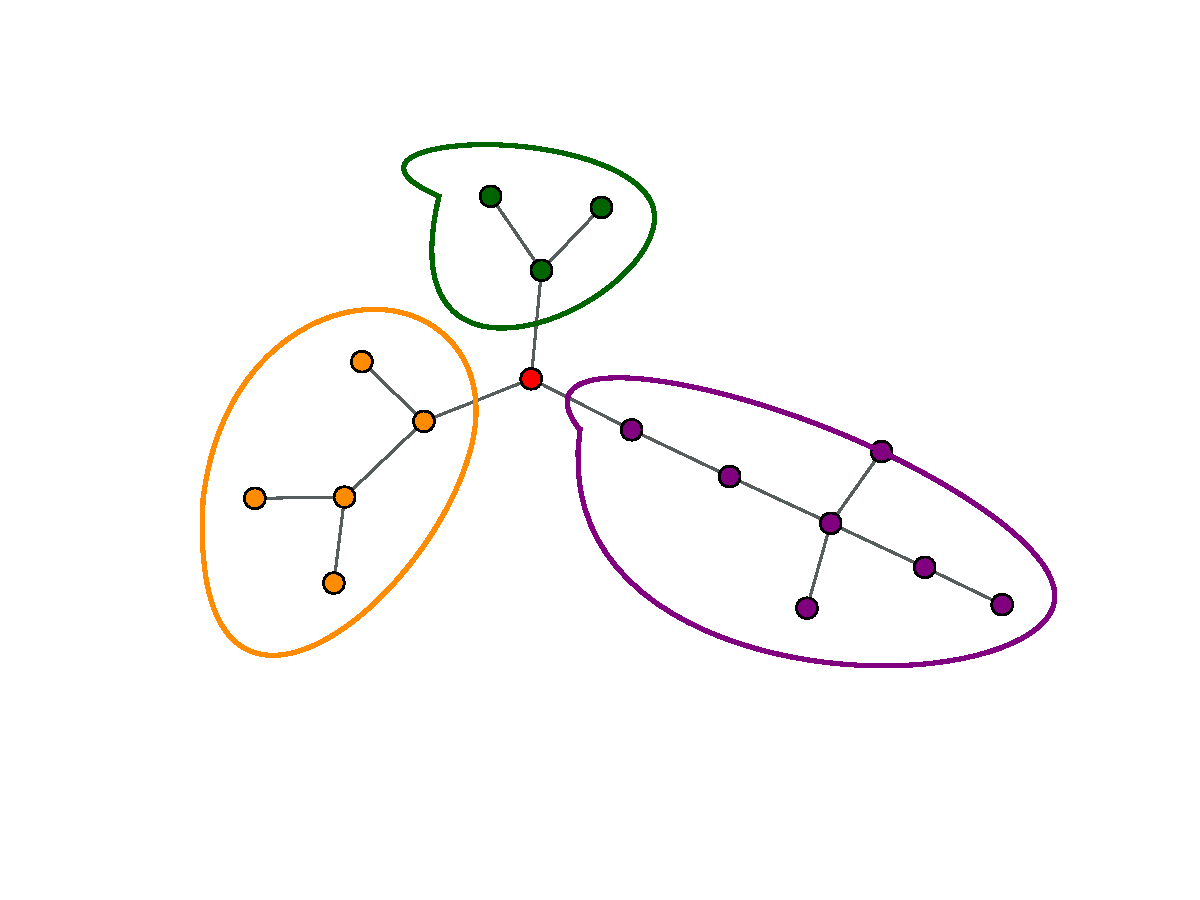
\includegraphics[width=\columnwidth]{cavity.pdf}
\end{frame}
%-------------------------
%-------------------------
\begin{frame}
    \frametitle{}
    \centering
    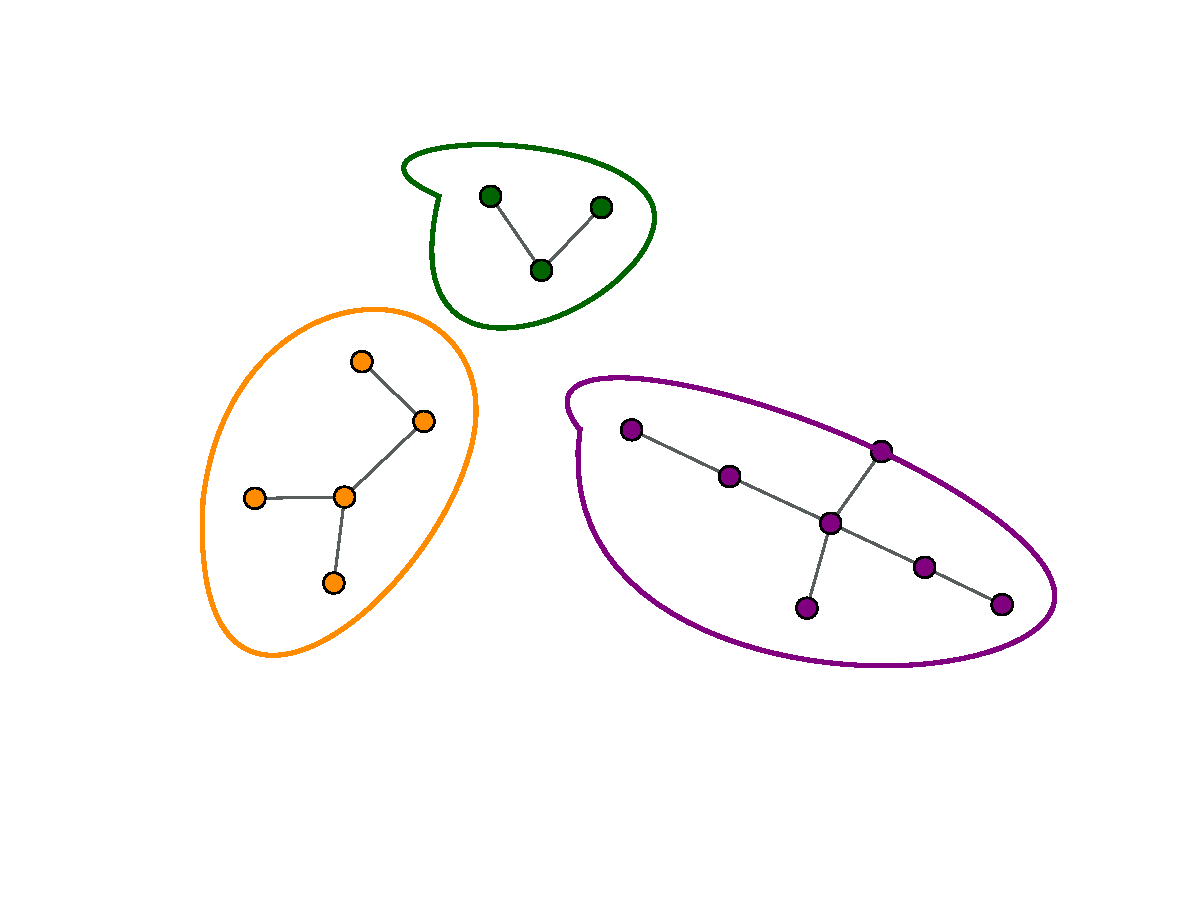
\includegraphics[width=\columnwidth]{cavity2.pdf}
\end{frame}
%-------------------------
%-------------------------
\begin{frame}
    \frametitle{}
For degree $3$ vertex, 
    $$\mathlarger{P(s|k=3) = \pi_{s_1}\pi_{s_2}\pi_{s_3}}$$
    $$s_1 + s_2 + s_3 = s-1$$
\pause
\justifying
$$P(s|k) = \sum\limits_{s_1=0}^{\infty}\sum\limits_{s_2=0}^{\infty}\cdots\sum\limits_{s_k=0}^{\infty}\left[\prod\limits_{j=1}^k\pi_{s_j}\right]\delta(s-1, \sum\limits_js_j)$$
\pause
$$\pi_s = \sum\limits_{k=0}^{\infty}p_kP(s|k)$$
$$<s> = \sum\limits_{s=0}^\infty s\pi_s$$
\end{frame}
%-------------------------
%-------------------------
\begin{frame}
    \frametitle{}
    \begin{columns}
        \column{0.5\linewidth}
    $$<s> = \frac{1}{1-c+cS}$$
        \vspace{2em}
        \pause
    $$R = \frac{2}{2-c+cS}$$
        \column{0.6\linewidth}
    \centering
        \pause
        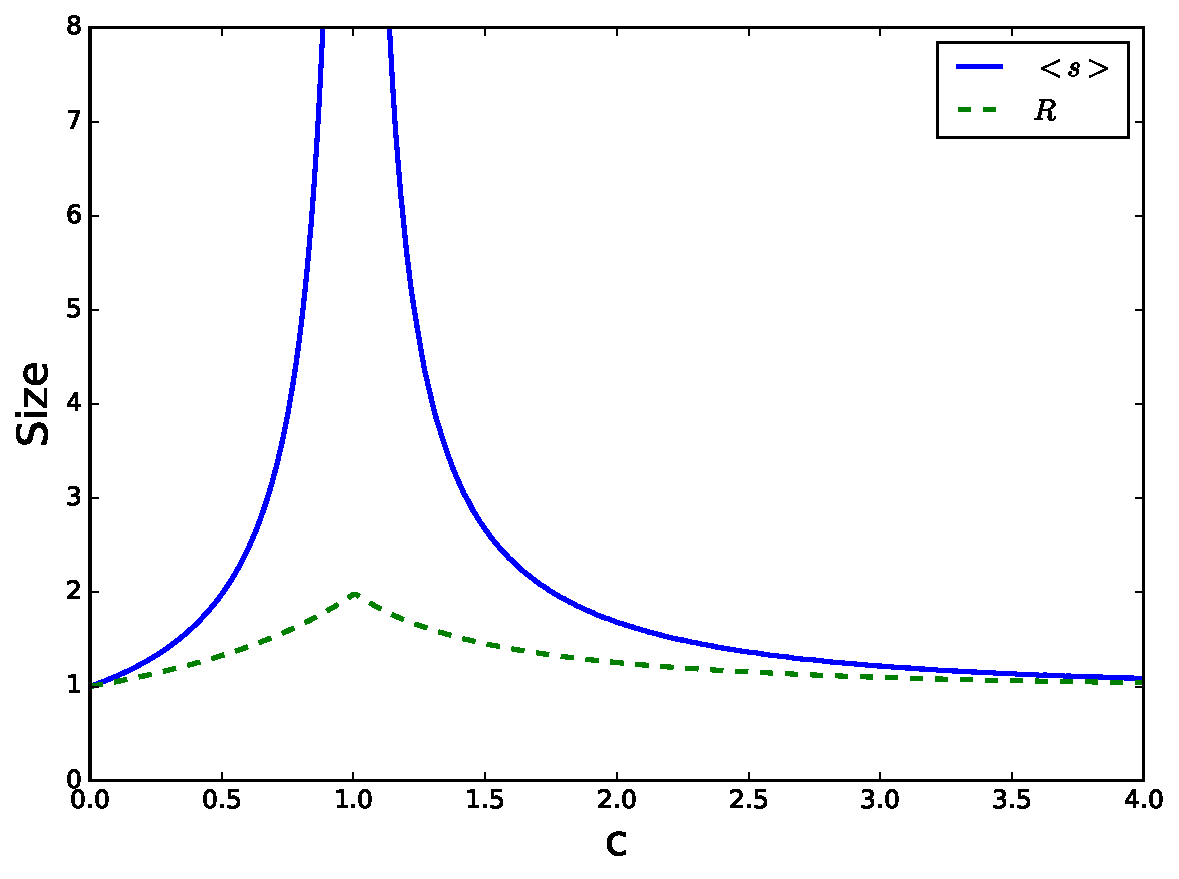
\includegraphics[width=\columnwidth]{average_small_comp.pdf}
    \end{columns}
\end{frame}
%-------------------------
%-------------------------
\begin{frame}
    \frametitle{Configuration model}
    \centering
    \begin{itemize}
    \setlength\itemsep{1em}
        \item{Model with a given degree sequence}
        \item{More realistic and more flexible}
        \item{Can be solved exactly in the limit}
    \end{itemize}
\end{frame}
%-------------------------
%-------------------------
\begin{frame}
    \frametitle{Configuration model}
    \begin{columns}
    \column{0.6\linewidth}
    \begin{itemize}
    \setlength\itemsep{1em}
        \item{Specify $k_i$ for $i=1, 2, \cdots, n$}
        \item{Every vertex $i$ has $k_i$ half-edges/stubs}
        \item{$\sum\limits_i k_i = 2m$}
        \item{Randomly connect stubs to each other}
        \item{Every matching appears with equal probability}
    \end{itemize}

    \column{0.4\linewidth}
    \centering
    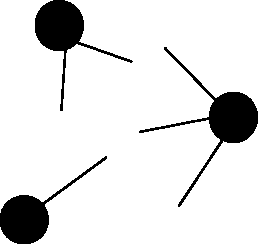
\includegraphics[width=0.8\columnwidth]{configuration.pdf}
    \note{self-loops and multiedges}
    \end{columns}
\end{frame}
%-------------------------
%-------------------------
\begin{frame}
    \frametitle{Configuration model}
    \centering
    \vspace{2em}
    {\bf Do all graphs appear with equal probability?}

    \pause
    \vspace{1em}
    More than one matchings can correspond to the same graph
    %\vspace{2em}
    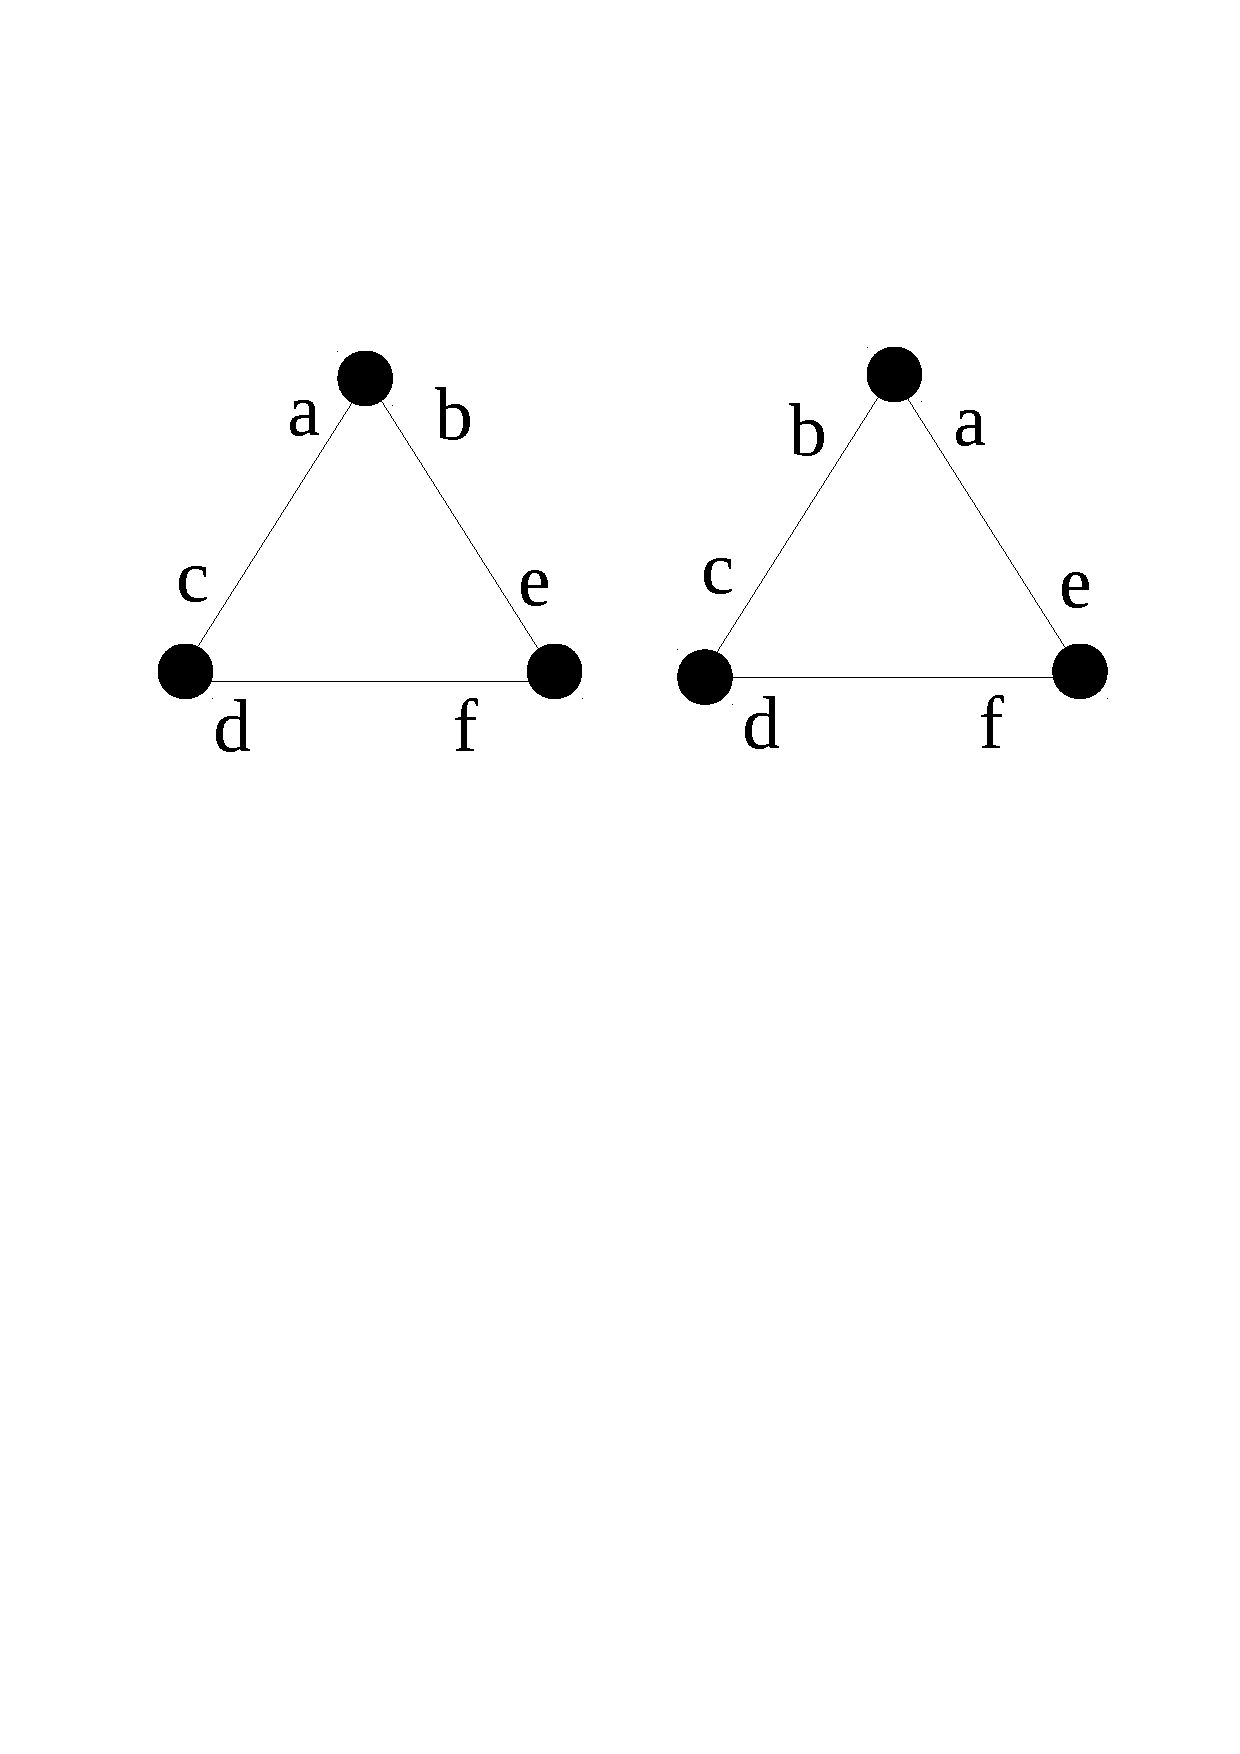
\includegraphics[width=0.8\columnwidth,trim = 0 200 0 80, clip = true]{triangle.pdf} 
\end{frame}
%-------------------------
%-------------------------
\begin{frame}
    \frametitle{Configuration model}
    \centering
    Number of matchings for the network $N$: $N(\{k_i\}) = \prod_ik_i!$\\

    \vspace{2em}
    Thus, networks do occur with equal probability!
\end{frame}
%-------------------------
%-------------------------
\begin{frame}
    \frametitle{Configuration model}
    \centering
    \includegraphics[width=\columnwidth]{dumbelled.pdf}
\end{frame}
%-------------------------
%-------------------------
\begin{frame}
    \frametitle{Configuration model}
    \centering
    $$N = \frac{\prod_i k_i!}{\prod_{i<j}A_{ij}!\prod_i A_{ii}!!}$$

    \vspace{2em}
    $$n!! = n(n-2)(n-4)\cdots 2$$

    \vspace{2em}
    Graphs do not appear with equal probability!
\end{frame}
%-------------------------
%-------------------------
\begin{frame}
    \frametitle{Summary}
    \centering
    \begin{itemize}
    \setlength\itemsep{1em}
        \item{Many real networks have fat-tailed degree distributions}
        \item{Naturally occuring networks tend be dissortative by degree}
        \item{Social networks tend to be assortative by degree}
        \item{Random graphs provide a powerful way to describe the large-scale structure of complex networks}
    \end{itemize}
\end{frame}
%-------------------------
\end{document}
